\documentclass[11pt,a4paper]{scrbook}
\usepackage[utf8]{inputenc}
\usepackage[T1]{fontenc}
\usepackage[english]{babel}
\usepackage{lmodern}
\usepackage{tikz}
\usepackage[margin=1.2in]{geometry}
\usepackage{amsmath}
\usepackage{amsthm}
\usepackage{hyperref}
\usepackage{mathpartir}
\usepackage{tikz}
\usepackage{amssymb}
\usepackage{latexsym}
\usepackage{syntax}
\usepackage{lscape}
\usepackage{stmaryrd}
\usepackage{listings}
\usepackage{newunicodechar}
\usepackage{xspace}
\usepackage[labelsep=period, labelfont=bf]{caption}

\makeatletter
\newcommand*{\shifttext}[2]{%
    \settowidth{\@tempdima}{#2}%
    \makebox[\@tempdima]{\hspace*{#1}#2}%
}
\makeatother

\newunicodechar{≠}{=\llap{/}}
\newunicodechar{≔}{:\raisebox{-0.18ex}[\height][\depth]{=}}
\newunicodechar{∧}{\shifttext{0.4ex}{/}\shifttext{-0.4ex}{\textbackslash}}

% CODE LISTINGS

\definecolor{cogreen}{RGB}{0,80,0}
\lstset{
    language=Java,
    basicstyle=\ttfamily\small,
    commentstyle=\ttfamily,
    frame=single,
    framesep=5pt,
    mathescape=true,
    %escapeinside={(*}{*)},
    keywordstyle=\color{blue}\ttfamily,
    stringstyle=\color{darkgray}\ttfamily,
    commentstyle=\color{cogreen}\ttfamily,
    morekeywords={requires, ensures}
}

% THEOREMS
\newtheorem{definition}{Definition}[section]
\newtheorem{theorem}[definition]{Theorem}
\newtheorem{lemma}[definition]{Lemma}
\newtheorem{corollary}[definition]{Corollary}

% BIB
\bibliographystyle{plain}

% COMMANDS
% \DeclareMathSymbol{\mlq}{\mathord}{operators}{``}
% \DeclareMathSymbol{\mrq}{\mathord}{operators}{`'}
\DeclareMathOperator*{\argmin}{\arg\!\min}
\DeclareMathOperator*{\argmax}{\arg\!\max}

%% decoration
\newcommand{\pa}[1]{\ensuremath{{#1}^{\checkmark}}}
\newcommand{\pb}[1]{\ensuremath{{#1}^{\circ}}}

\newcommand{\grad}[1]{\widetilde{#1}}
\newcommand{\dgrad}[1]{\vec{#1}}

%% ALIASES
% fonts
\newcommand{\std}{\textrm}
\newcommand{\ttt}{\texttt}
\newcommand{\tset}{\textsc}
\newcommand{\predicate}[1]{\textup{\textsf{#1}}}
% names
\newcommand{\gsvl}{\std{GSVL}\xspace}
\newcommand{\svl}{\std{SVL}\xspace}
\newcommand{\dvl}{\std{DVL}\xspace}
\newcommand{\gvl}{\std{GVL}\xspace}

% sets
\newcommand{\setProgramState}{\tset{ProgramState}\xspace}
\newcommand{\setProgramStateFin}{\tset{ProgramStateFin}\xspace}
\newcommand{\setProgramStateEx}{\tset{ProgramStateEx}\xspace}
\newcommand{\setGProgramState}{\tset{GProgramState}\xspace}
\newcommand{\setGProgramStateFin}{\tset{GProgramStateFin}\xspace}
\newcommand{\setGProgramStateEx}{\tset{GProgramStateEx}\xspace}
\newcommand{\setProgram}{\tset{Program}\xspace}
\newcommand{\setGProgram}{\tset{GProgram}\xspace}
\newcommand{\setClass}{\tset{Class}\xspace}
\newcommand{\setField}{\tset{Field}\xspace}
\newcommand{\setMethod}{\tset{Method}\xspace}
\newcommand{\setGMethod}{\tset{GMethod}\xspace}
\newcommand{\setContract}{\tset{Contract}\xspace}
\newcommand{\setGContract}{\tset{GContract}\xspace}
\newcommand{\setType}{\tset{Type}\xspace}
\newcommand{\setStmt}{\tset{Stmt}\xspace}
\newcommand{\setGStmt}{\tset{GStmt}\xspace}
\newcommand{\setStmts}{\tset{Stmts}\xspace} %TODO!!!
\newcommand{\setFormula}{\tset{Formula}\xspace}
\newcommand{\setFormulaA}{\tset{SatFormula}\xspace}
\newcommand{\setFormulaB}{\tset{SfrmFormula}\xspace}
\newcommand{\setGFormula}{\tset{GFormula}\xspace}
\newcommand{\setGFormulaA}{\tset{SatGFormula}\xspace}
\newcommand{\setGFormulaB}{\tset{SfrmGFormula}\xspace}
\newcommand{\setExpr}{\tset{Expr}\xspace}
\newcommand{\setVal}{\tset{Val}\xspace}
\newcommand{\setObj}{\tset{Obj}\xspace}
\newcommand{\setVar}{\tset{Var}\xspace}

\newcommand{\setHeap}{\tset{Heap}\xspace}
\newcommand{\setStack}{\tset{Stack}\xspace}
\newcommand{\setStackEntry}{\tset{StackEntry}\xspace}
\newcommand{\setVarEnv}{\tset{VarEnv}\xspace}
\newcommand{\setTypeEnv}{\tset{TypeEnv}\xspace}
\newcommand{\setClassName}{\tset{ClassName}\xspace}
\newcommand{\setFieldName}{\tset{FieldName}\xspace}
\newcommand{\setMethodName}{\tset{MethodName}\xspace}
\newcommand{\setSFootprint}{\tset{StaticFootprint}\xspace}
\newcommand{\setDFootprint}{\tset{DynamicFootprint}\xspace}
% expressions
\newcommand{\ev}[1]{\ttt{#1}}
\newcommand{\ex}[1]{\ttt{#1}}
\newcommand{\edot}[2]{\ttt{#1.#2}}
\newcommand{\ethis}{\ex{this}}
\newcommand{\eresult}{\ex{result}}
\newcommand{\enull}{\ttt{null}}
% formulas
\newcommand{\phiAnd}[2]{\ttt{#1\:∧\:#2}}
\newcommand{\phiCons}[2]{\ttt{#1\:*\:#2}}
\newcommand{\phiFalse}[0]{\ttt{false}}
\newcommand{\phiTrue}[0]{\ttt{true}}
\newcommand{\phiEq}[2]{\ttt{(#1 = #2)}}
\newcommand{\phiNeq}[2]{\ttt{(#1 ≠ #2)}}
\newcommand{\phiAcc}[2]{\ttt{acc(#1.#2)}}
\newcommand{\qm}{\ttt{?}}
\newcommand{\withqm}[1]{\phiCons{\qm}{\ensuremath{#1}}}
\newcommand{\withqmGen}[1]{\phiAnd{\ensuremath{#1}}{\qm}}
% statements
\newcommand{\sSkip}{\ttt{skip}}
\newcommand{\sFieldAssign}[3]{\ttt{#1.#2 ≔ #3}}
\newcommand{\sVarAssign}[2]{\ttt{#1 ≔ #2}}
\newcommand{\sAlloc}[2]{\ttt{#1 ≔ new #2}}
\newcommand{\sCall}[4]{\ttt{#1 ≔ #2.#3(#4)}}
\newcommand{\sReturn}[1]{\ttt{return #1}}
\newcommand{\sAssert}[1]{\ttt{assert #1}}
\newcommand{\sRelease}[1]{\ttt{release #1}}
\newcommand{\sDeclare}[2]{\ttt{#1~#2}}
\newcommand{\sHold}[2]{\ttt{hold #1~\{ #2 \}}}
\newcommand{\sSeq}[2]{\ttt{{#1};{#2}}}
% type
\newcommand{\type}[1]{\ttt{#1}}
\newcommand{\Tint}{\type{int}}
% composite syntax
\newcommand{\class}[3]{\ttt{class {#1}~\{ {#2} {#3} \}}}
\newcommand{\method}[6]{\ttt{{#1}~{#2}({#3}~{#4})~{#5}~\{ {#6} \}}}
\newcommand{\contract}[2]{\ttt{requires {#1}; ensures {#2};}}
\newcommand{\field}[2]{\ttt{{#1}~{#2};}}
%% predicates
% precision
\newcommand{\mpt}{\sqsubseteq}
\newcommand{\mptpi}{\sqsubseteq_{\pi}}
% well-formed
\newcommand{\wsp}{\predicate{wsp}}
\newcommand{\verify}{\predicate{verify}}
\newcommand{\OK}{~\predicate{OK}}
\newcommand{\OKinC}{~\predicate{OK in}~C}
% framing
\newcommand{\sfrme}{\ensuremath{\vdash_\texttt{frm}}\,}
\newcommand{\sfrmphi}{\ensuremath{\vdash_\texttt{sfrm}}\,}
% evaluation
\newcommand{\evalex}[4]{#1,#2 \vdash #3 \Downarrow #4}
\newcommand{\evale}[2]{H,\rho \vdash #1 \Downarrow #2}
\newcommand{\evalphiXGen}[2]{#1 \vDash_{X} #2}
\newcommand{\evalgphiXGen}[2]{#1 \,\,\grad{\vDash_{X}}\,\, #2}
\newcommand{\evalphiGen}[2]{#1 \vDash #2}
\newcommand{\evalgphiGen}[2]{#1 \,\,\grad{\vDash}\,\, #2}
\newcommand{\evalphi}[1]{\evalphiGen {H,\rho,A} {#1}}
\newcommand{\evalgphi}[1]{\evalgphiGen {H,\rho,A} {#1}}
\newcommand{\phiImplies}[2]{{#1} \underset{\phi}{\implies} {#2}}
\newcommand{\gphiImplies}[2]{{#1} \,\,\underset{\phi}{\grad{\implies}}\, {#2}}
\newcommand{\evalphix}[4]{\evalphiGen {#1,#2,#3} {#4}}
% extraction
\newcommand{\fieldType}{\predicate{fieldType$_p$}}
\newcommand{\fields}{\predicate{fields$_p$}}
\newcommand{\mpre}{\predicate{mpre$_p$}}
\newcommand{\mpost}{\predicate{mpost$_p$}}
\newcommand{\mmethod}{\predicate{method$_p$}}
% other
\newcommand{\static}{\predicate{static}}
\newcommand{\dom}{\predicate{dom}}
\newcommand{\writesTo}{\predicate{writesTo}}
\newcommand{\sType}[3]{{#1} \vdash {#2} : {#3}}
\newcommand{\defaultValue}[1]{\predicate{defaultValue(#1)}}
\newcommand{\defeq}{\overset{\predicate{def}}{=}}
\newcommand{\defiff}{\overset{\predicate{def}}{\iff}}
\newcommand{\accFor}[1]{\llbracket #1 \rrbracket}
% footprint
\newcommand\floor[1]{\lfloor#1\rfloor}
\newcommand\ceil[1]{\lceil#1\rceil}
\newcommand{\staticFP}[1]{\ensuremath{\floor{#1}}}
\newcommand{\dynamicFP}[3]{\ensuremath{\floor{#3}_{#1,#2}}}
% static sem
\newcommand{\hoare}[3]{\{{#1}\} ~{#2}~ \{{#3}\}}
\newcommand{\thoare}[4]{{#1} \vdash \{{#2}\} ~{#3}~ \{{#4}\}}
\newcommand{\gthoare}[4]{{#1} \,\,\grad{\vdash}\,\, \{{#2}\} ~{#3}~ \{{#4}\}}
\newcommand{\dgthoare}[4]{{#1} \,\,\dgrad{\vdash}\,\, \{{#2}\} ~{#3}~ \{{#4}\}}
\newcommand{\PP}{\mathcal{P}}
\newcommand{\sssem}{\mathcal{S}}
\newcommand{\gsssem}{\grad{\sssem}}
\newcommand{\funHoare}{\mathcal{H}}
\newcommand{\funHoareA}{\mathcal{F}}
\newcommand{\funHoareApred}{\mathcal{P}}
\newcommand{\funHoareB}{\mathcal{I}}
\newcommand{\funHoareBimp}{\mathcal{J}}
\newcommand{\funHoareC}{\mathcal{M}}
% dyn sem
\newcommand{\progress}{\predicate{progress}_{\sssem}}
\newcommand{\sstepGeneric}[5]{({#1}, {#2}) \rightarrow^{#3} ({#4}, {#5})}
\newcommand{\sstep}[4]{\sstepGeneric {#1} {#2} {} {#3} {#4}}
\newcommand{\ssteps}[4]{\sstepGeneric {#1} {#2} * {#3} {#4}}

\newcommand\restr[2]{{% we make the whole thing an ordinary symbol
        \left.\kern-\nulldelimiterspace % automatically resize the bar with \right
        #1 % the function
        \vphantom{\big|} % pretend it's a little taller at normal size
        \right|_{#2} % this is the delimiter
    }}



\begin{document}

% 1. Front pages
\pagenumbering{gobble}
\begin{titlepage}
	\usetikzlibrary{positioning,calc}
    \begin{tikzpicture}[remember picture,overlay]
      % Seitenrahmen zeichnen.
      \draw[semithick,rounded corners=0.5cm]
        ($(current page.north west) + ( 1cm,-1cm)$) --
        ($(current page.north east) + (-1cm,-1cm)$) --
        ($(current page.south east) + (-1cm, 1.5cm)$);
        
      \draw[semithick,rounded corners=0.5cm]
        ($(current page.south east) + (-1cm, 1.5cm)$) --
        ($(current page.south west) + ( 1cm, 1.5cm)$) --
        ($(current page.north west) + ( 1cm,-1cm)$);
        
      % Logo einbinden.
      \node[anchor=north west] (logo1) at ($(current page.north west) + (1.75cm,-1.5cm)$)
      {
        \begin{minipage}{2.125in}
            
\includegraphics[width=4.5cm]{logos/KIT}
            \begin{flushleft}
                \footnotesize{}
                Institute for Program Structures\\
                and Data Organization (IPD) \\
            \end{flushleft}
        \end{minipage}
      };
      
      % Institut / Lehrstuhl.
      \node[anchor=north east] at ($(current page.north east) + (-1.75cm,-1.5cm)$)
      {    
          \begin{minipage}{2.125in}
              %
\includegraphics[width=4cm]{logos/cmu-stacked}
              
\includegraphics[width=2.125in]{logos/cmu-flat}
              ~\\
              
\includegraphics[width=2.125in]{logos/ISR}
          \end{minipage}
      };
      
      \node (title) at ($(current page.center) + (0cm, 6cm)$)
      {
        % Korrekter Zeilenabstand etc. durch Minipage.
        \begin{minipage}{12cm}
          \begin{center}
            \huge\textbf{Gradual Program Verification with Implicit Dynamic Frames}
          \end{center}
        \end{minipage}
      };
      
      \node[below=1.75cm of title.south]   (prename)  { Master's Thesis of };
      \node[below=0.75cm of prename.south] (name)     { \Large{}\textbf{Johannes Bader} };
      \node[below=1cm    of name.south]    (postname1) { presented to the Department of Informatics };
      \node[below=1.5cm    of name.south]    (postname2) { Institute for Program Structures
and Data Organization (IPD) };
      
      \node[below=4.5cm of postname1.south] (table)
      {
        \begin{tabular}{ll}
        \textbf{Advisor:}       & Prof. Jonathan Aldrich, Carnegie Mellon University - Pittsburgh, USA \\
        \textbf{Advisor:}       & Prof. Éric Tanter, University of Chile - Santiago, Chile \\
        \textbf{Co-Advisor:}    & Prof. Dr.-Ing. Gregor Snelting, Karlsruhe Institute of Technology - Karlsruhe, Germany \\[5pt]

                                           
        \end{tabular}
      };
      
      \node[below=4.5cm of table.south] (time)
      {
        \begin{tabular}{ll}
        \textbf{Duration:} & 2016-05-10 -- 2016-10-04
        \end{tabular}
      };
      
      % Fußzeile, unten zentriert.
      \node[anchor=south] (footnote) at ($(current page.center |- current page.south) + (0cm, 0.65cm)$)
      {
        \tiny{}KIT -- University of the State of Baden-Wuerttemberg and National Research Center of the Helmholtz Association
        \hspace{0.5cm}
        \Large{}\textbf{www.kit.edu}
      };
    \end{tikzpicture}
\end{titlepage}

\vspace*{33\baselineskip}
\hbox to \textwidth{\hrulefill}
\par
I declare that I have developed and written the enclosed thesis completely by myself, and have not used sources or means without declaration  in the text, and have followed the rules of the KIT for upholding good scientific practice.\\

\textbf{Karlsruhe, 2016-??-??}
\vspace{1.5cm}
 
\dotfill\hspace*{8.0cm}\\
\hspace*{2cm}(\textbf{Johannes Bader}) %center name with hspace


\begin{center}
\begin{minipage}{0.7\textwidth}
\vspace*{15\baselineskip}
\begin{center}
\textbf{Abstract}
\end{center}
% Purpose/Problem
%Methods of program verification can traditionally be categorized as either static or dynamic.
%Static verification uses formal methods like Hoare logic to guarantee conformance with a given specification without running the program.
%Dynamic verification uses runtime checks to ensure that deviations from the specification are detected during execution.
Both static and dynamic program verification approaches have disadvantages potentially disqualifying them as a single methodology to rely on.
% Proposal/Methods
Motivated by gradual type systems, which solve a very similar dilemma in the world of type systems, we propose \textit{gradual verification}, an approach that seamlessly combines static and dynamic verification.
Drawing on principles from abstract interpretation and recent work on \textit{abstracting gradual typing} by Garcia, Clark and Tanter, we formalize how to obtain a gradual verification system in terms of a static one.

% Results
This approach yields \textit{by construction} a verification system that is compatible with the original static system, but overcomes its rigidity by resorting to methods of dynamic verification if necessary.
% gradual guarantee
In a case study, we show the flexibility of our approach by applying it to a concurrent statically verified language that uses implicit dynamic frames to enable race-free reasoning.
\end{minipage}
\end{center}


\vspace*{15\baselineskip}
\textbf{Acknowledgments}\\\\
I wish to thank my advisors Jonathan Aldrich and Éric Tanter for offering me this topic and for their patient assistance throughout the past few months. In any situation and every way, their remarks and thoughts guided me in the right direction.\\\\
Also I am very grateful to all my family and friends who encouraged and supported me throughout my life.


% 2. TOC
\tableofcontents

% 3. Content
\pagenumbering{arabic}
% IDEA: separate theoretical/general approach and concrete decisions
% this means, for example, that:
% PART1:
% - requirements for lifted functions, soundness
% - implication (gradual, ...)
% - abstract versions of [w/o], append
% PART2:
% - concrete version of [w/o], append, ... (probably requires notion of normalized env :( )
% - actual implementation

\chapter{Introduction}
\label{ch:introduction}
%% program verification
Program verification aims to check a computer program against its specification.
Automated methods require this specification to be formalized, e.g. using annotations in the source code.
Common examples are method contracts, loop invariants and assertions.

%% static vs dynamic
Approaches to check whether program behavior complies with given annotations can be divided into two categories:
\begin{description}
    \item[Static verification]~\\
        The program is not executed. 
        Instead \emph{formal methods} (like Hoare logic or separation logic) are used, trying to derive a proof for given assertions.
        
        \textbf{Drawbacks}\\
        The syntax available for static verification is naturally limited by the underlying formal logic.
        Complex properties (e.g. including database lookups or library calls) might thus not be expressible, resulting in inability to prove subsequent goals.
        Furthermore, the logic itself might fail proving certain goals due to code complexity and undecidability in general.
        Using static verification usually requires rigorous annotation of the entire source code, as otherwise there might be too little information to find a proof.
        While fully annotating own code can be tedious (there are supporting tools), using unannotated libraries can become a problem:
        Even if it is possible to annotate the API afterwards, lacking the source code the verifier is unable to prove those annotations.
        In case the annotations are wrong this results in inconsistent proofs.
        
    \item[Dynamic verification]~\\
        The specification is turned into \emph{runtime checks}, making sure that the program adheres to its specification during execution.
        Violations cause a runtime exception to be thrown, effectively preventing the program from entering a state that contradicts its specification.
        Note that in practice this approach is often combined with control flow based testing techniques to detect misbehavior as early as possible.
        
        \textbf{Drawbacks}\\
        Violations are only detected at runtime, with the risk of going unnoticed before software is released.
        To minimize this risk, testing methods are required, i.e. more time has to be spent after compilation.
        The usage of runtime checks naturally imposes a runtime overhead which is not always acceptable.
\end{description}

The goal of this work is to formalize “gradual verification”, an approach that seamlessly combines static and dynamic verification in order to weaken or even avoid above drawbacks by introducing an “unknown” formula $\qm$.
The resulting system provides a continuum between traditional static and dynamic verification, meaning that both extremes are compatible with, but only special cases of the gradual verification system.
Section \ref{sec:motivationexamples} gives example scenarios of both static and dynamic verification suffering from their drawbacks, illustrating how gradual verification could avoid them.
% Programmers

Our approach is based on recent advances in formalizing gradual typing, specifically “Abstracting Gradual Typing” \cite{garcia2016abstracting} by Garcia, Clark and Tanter.
They describe a process called “gradualization” that uses the concept of abstract interpretation to define a gradual system in terms of a static one.
Gradual typing emerged from drawbacks of static and dynamic type systems that are very similar to the drawbacks of verification systems outlined above.
This is no surprise from a theoretical perspective as type systems are a special case of program verification. 
These similarities motivated our idea of reinterpreting and adapting the gradual typing approach to the verification setting.

Chapter \ref{sec:categorization-of-existing} introduces the concepts motivating and driving our approach.
Furthermore it categorizes existing work that goes in a similar direction, pointing out how it differs from our work.
In chapter \ref{ch:gradualization-of-a} we describe our approach of gradualization in a generic way, meant to be used as a manual or template for designing gradual verification systems.
We follow that manual in form of a case study in chapter \ref{ch:case-study--implicit}, applying the approach to a statically verified language that uses implicit dynamic frames in order to enable safe static reasoning about shared mutable state.
We conclude with an evaluation of our approach (chapter \ref{ch:evaluation-analysis}) and a conclusion (chapter \ref{ch:conclusion}).
The appendix contains additional information like proofs. % TODO: is that all?
We have also implemented the gradually verified language developed in chapter \ref{ch:case-study--implicit} as a web page (see section \ref{sec:implementation}).

\begin{comment}

Most modern programming languages use static methods to some degree, ruling out at least some types of runtime failure.
%% static typing
Static typing disciplines are among the most common representatives, guaranteeing type safety at compile time, obviating the need for dynamic checks.
Yet, the rigidity and limitations of static type systems resulted in the introduction of dynamic aspects into the otherwise static system:
Casts (e.g. as implemented in C\# or Java) overrule purely static reasoning, allowing the static type system to treat an expression as if it had the claimed type (usually a subtype) instead of the deduced one.
At this location, a runtime check is introduced, resulting in a cast exception should the programmer's claim turn out wrong.
Note that such deviations from a purely static type system (one where there is no need for runtime checks) do not affect type safety:
It is still guaranteed that execution does not enter an inconsistent state by simply interrupting execution whenever a runtime type check fails.

Note that casts are necessary only because of a typical drawback of static systems, namely the limitation of the underlying logic.
More sophisticated type systems (e.g. the one in Haskell) might have been able to deduce the claimed type in the first place.

%% dynamic typing
%At the other end of the spectrum are dynamically typed languages.
%In scenarios where the limitations of a static type system would clutter up the source code, they allow expressing the same logic with less %syntactic overhead, but at the cost of less static guarantees and early bug detection.

%% static verification
In contrast, general purpose static verification techniques are not common amongst popular programming languages.
Note that such languages are usually driven by cost-benefit and usability considerations, meaning that static verification is apparently not yet in a stage where its cost clearly outweighs its benefits.
\end{comment}

\begin{comment}
%% static verification
% example?

% D even has both

% this is more of a consequence of the “deep roots” of dynamic verification!!!
%But even preconditions at expression level are implemented as runtime checks, reflected all the way down at instruction architecture level.
%Examples:
%\begin{description}
%    \item[Division by zero]~\\
%    Integer division performs a dynamic check...
%    
%\end{description}

- 
What is the thesis about?
Why is it relevant or important?
What are the issues or problems?
What is the proposed solution or approach?
What can one expect in the rest of the thesis?

“Static verification checks that properties are always true, but it can be difficult and tedious to select a goal and to annotate programs for input to a static checker.” (http://www.sciencedirect.com/science/article/pii/S1571066104002567)
\end{comment}

    \section{Motivational Examples}
    \label{sec:motivationexamples}
    
\subsection{Argument Validation}
The following Java example motivates the use of verification for argument validation.
\begin{lstlisting}
boolean hasLegalDriver(Car c)
{
    // business logic:
    resAllocate();
    boolean result = c.driver.age >= 18;
    resFree();
    return result;
}
\end{lstlisting}
A call to \ttt{hasLegalDriver} fails if \ttt{c} or \ttt{c.driver} evaluate to \ttt{null}.
Note that, although the Java runtime has defined behavior in to those cases (throwing an exception), we might still have created a resource leak.
To prevent this from happening, arguments have to be validated before entering the business logic.
\begin{lstlisting}
boolean hasLegalDriver(Car c)
{
    if (!(c != null))
        throw new IllegalArgException("expected c != null");
    if (!(c.driver != null))
        throw new IllegalArgException("expected c.driver != null");
        
    // business logic (requires 'c.driver.age' to evaluate)
}
\end{lstlisting}

Note that these runtime checks dynamically verifies a method contract, having \ttt{c != null \&\& c.driver != null} as precondition.
Naturally, the drawbacks of dynamic verification apply:
Violations of the method contract are only detected at runtime, possibly go unnoticed for a long time and impose a runtime overhead which might not be acceptable in all scenarios.
Java even has dedicated assertion syntax simplifying dynamic verification:
\begin{lstlisting}
boolean hasLegalDriver(Car c)
{
    assert c != null;
    assert c.driver != null;

    // business logic (requires 'c.driver.age' to evaluate)
}
\end{lstlisting}
Note however that such assertions are dropped from regular builds, meaning that the method contract is no longer verified!

With support of additional tools, a more declarative approach is possible using JML syntax:
\begin{lstlisting}
//@ requires c != null && c.driver != null;
boolean hasLegalDriver(Car c)
{
    // business logic (requires 'c.driver.age' to evaluate)
}
\end{lstlisting}

There are two basic ways to turn this annotation into a guarantee:
\begin{description}
    \item[Static Verification (e.g. ESC/Java, see \cite{leino2000esc})]~\\
    Verification will only succeed if the precondition is provable at all call sites.
    This is achievable in two ways:
    \begin{itemize}
        \item
        Rigorously annotate the call sites, guiding the verifier towards a proof.
        \item 
        Add parameter validation to the call sites, effectively duplicating the original runtime check across the program.
        Note that this approach combines static and dynamic validation in order to get a performance benefit (no more runtime checks required where precondition was provable) and circumvent rigorous annotation.
        The drawback is of course code duplication.
    \end{itemize}
    % benefits, drawbacks
    
    %There are obvious limitations to this approach, static verification tends to be invasive.
    %At least there is a performance benefit: 
    %Runtime checks (originally part of every call) are now only necessary in places where verification would not succeed otherwise.
    
    \item[Dynamic Verification (e.g. run JML4c, see \cite{sarcar2010new}]~\\
    This approach basically converts the annotation back into a runtime check equivalent to our original argument validation.
    % benefits, drawbacks
\end{description}

Gradual verification would pursue the combined approach without (visible) code duplication:
Static verification is used where possible, dynamic verification where needed.
Note that for the programmer this means that adding the method contract comes with no further obligations.

\subsection{Limitations of Static Verification}
The following example is written in a Java-like language with dedicated syntax for method contracts (similar to Eiffel and Spec\#).
We assume that this language is statically verified, i.e. static verification is part of the compilation.

The example shows the limitations of static verification using the Collatz sequence as an algorithm too complex to describe concisely in a method contract:
\begin{lstlisting}
int collatzIterations(int iter, int start)
    requires 1 <= start;
    ensures  1 <= result;
{
    // ...
}

int myRandom(int seed)
    requires 1 <= seed   && seed   <= 10000;
    ensures  1 <= result && result <= 3;     // not provable
{
    int result = collatzIterations(300, seed);
    // we know:        result $\in$ { 1, 2, 4 }
    // verifier knows: 1 <= result
    
    if (result == 4) result = 3;
    return result;
}
\end{lstlisting}
The first method \ttt{collatzIterations} iterates given number of times, starting at given value.
We assume that the only provable contract is that positive start value results in positive result.
The second method \ttt{myRandom} uses the Collatz sequence to generate a pseudo random number from given seed.
It is known to the programmer that start values up to 10000 result in convergence of the sequence after 300 iterations.
After mapping 4 to 3, we are thus given a number between 1 and 3, as described in the postcondition.

Unfortunately, the verifier cannot deduce this fact since the postcondition of \ttt{collatzIterations} only guarantees positive result, but no specific range of values.
Again, we can resort to dynamic methods to aid verification:

\begin{lstlisting}
...
{
    int result = collatzIterations(300, seed);
    // we know:        result $\in$ { 1, 2, 4 }
    // verifier knows: 1 <= result
    
    // knowledge "cast"
    if (!(result <= 4))
        throw new IllegalStateException("expected result <= 4");

    // verifier knows: 1 <= result && result <= 4 
    
    if (result == 4) result = 3;
    return result;
}
\end{lstlisting}

This solution is not satisfying as it required additional work by the programmer to convince the verifier.
Furthermore, the solution is in an unintuitive location:
The problem is not caused by \ttt{myRandom}, yet it is solved there.
The actual problem is that the postcondition of \ttt{collatzIterations} is too weak, causing the verifier to fail deducing our knowledge.

Gradual verification allows enhancing the postcondition with “unknown” knowledge that can be reinterpreted arbitrarily, adding appropriate runtime checks to guarantee that this reinterpretation was in fact valid:
\begin{lstlisting}
int collatzIterations(int iter, int start)
    requires 1 <= start;
    ensures  1 <= result && ?;
{
    // ...
}

int myRandom(int seed)
    requires 1 <= seed   && seed   <= 10000;
    ensures  1 <= result && result <= 3;
{
    int result = collatzIterations(300, seed);
    // we know: result $\in$ { 1, 2, 4 }
    
    // verifier allowed to
    //  assume 1 <= start && result <= 4
    //  from   1 <= start && ?
    // (adding runtime check)
    
    if (result == 4) result = 3;
    return result;
}
\end{lstlisting}
Note the \ttt{?} in the postcondition of \ttt{collatzIterations}.

% gradual:
% - not in a sense of GraVy
% - assertions are GUARANTEED not to be violated (analogous to type safety of gradually typed languages), meaning that
%    - as much as possible is verified statically
%    - if necessary, (ideally: as few as possible) dynamic checks kick in
% - full continuum between static and dynamic

% static checking
% dynamic checking
% combine static and dynamic checking
% views:
% - add designated "?" to statically checked language, making checking optional
% - introduce checking to unchecked language, making "?" the default value
% typing
% transition to verification
% - of particular interest, cause limitations due to syntax or decidability make full checking impossible,
%    possibly making use of static verification impossible and the program thus unverifiable
%    inevitable incompleteness of static verifiers!
%    GraVy: measure, only \textit{classifies} code into sections: correctness statically guaranteed, correctness statically disproved, no static guarantee so far

% very desirable in practice
% gradual version of a language is inherently a strict superset of original language
% 

% our approach allows extension of existing languages (without any verification) by adding transpilation step

% why would you want continuum?
% - move toward satically verified program without giving up guarantees!
% - while "barely typed" languages hardly make sense, programs with "little verification" are already highly useful
%    i.e. verification even makes sense as "rarely used feature"!
%    ArgumentException-example
%    -    performance benefit!
%    -    cleaner code!
%    -    makes more sense semantically
% having optional types 

% Future Work:
% implement on top of existing languages
% - tracking access via ThreadLocalStorage
% - transpilation (e.g. C# Roslyn compiler extension)



\chapter{Background}
\label{sec:categorization-of-existing}
Design-by-Contract, a term coined by Bertrand Meyer \cite{meyer2002design}, is a paradigm aiming for verifiable source code, e.g. by adding method contracts and tightly integrating them with the compiler and runtime.
Meyer implemented this concept in his programming language Eiffel \cite{meyer1988eiffel}, providing compiler support for generating runtime checks required for dynamic verification (also called runtime verification).
Combining design-by-contract with static verification techniques led to the concept of “verified design-by-contract” \cite{crocker2004safe}.

Similar developments took place regarding Java and JML specifications.
Static verification using theorem provers was investigated by Jacobs and Poll \cite{jacobs2001logic} and is implemented as part of ESC/Java \cite{nelson2004extended}.
Turning JML specifications into runtime assertion checks (RAC) to drive dynamic verification was described by Cheon and Leavens \cite{cheon2002runtime} and led up to the development of JML4c \cite{sarcar2010new}.

A more recent programming language with built-in support to express specifications, coming with both static and dynamic verification tools is Spec\# \cite{the-spec-programming-system-an-overview}.
Its compiler facilitates theorem provers for static verification and emits runtime checks for dynamic verification.
It was developed further to cope with the challenges of concurrent object-orientation \cite{a-statically-verifiable-programming-model-for-concurrent-object-oriented-programs}.
The concepts found their way to mainstream programming in the form of “Code Contracts” \cite{embedded-contract-languages}, a toolset deeply integrated with the Microsoft .NET framework and thus available in a variety of programming languages.

The limitations of both static and dynamic verification motivated a recent trend of using both approaches at the same time (as observable in the above programming languages).
Automated theorem provers are used to perform static verification as a best effort service rather than a requirement for successful compilation.
Their goal is to detect as many inconsistencies or contract violations as possible, but not necessarily find a proof for correctness.
So even if compliance with annotations cannot be proved programs are “optimistically accepted”.
Additionally, dynamic verification is used to restore the guarantee that static verification no longer provides.
% In other words, while traditional static verifiers either prove compliance with or violation of annotations, fail

Recent research focused on combining both approaches in a more meaningful and complementary way by focusing dynamic verification and testing efforts specifically to code areas where static verification had less success.
Christakis, Müller and Wüstholz \cite{ChristakisMuellerWuestholz16} describe how programs can be annotated during static verification in order to prioritize certain tests over others or even prune the search space by aborting tests that lead to fully verified code.

Still, static and dynamic verification concepts are treated as independent concepts for the most part.
The same was once true for static and dynamic type systems, before advances in formalizing gradual type systems seamlessly bridged the gap.
Our goal is to achieve the same for program verification, i.e. static and dynamic verification are no longer to be treated as independent concepts (that are then combined as intelligently as possible) but instead treated as one concept with different manifestations.

Note that Arlt et al. \cite{arlt2014gradual} mention “gradual verification”, yet it is meant as the process of gradually increasing the coverage of static verification.
The work describes a metric for estimating this coverage, giving the developer feedback while annotating programs.
A similar metric arises automatically from our notion of gradual verification: The number of dynamic checks injected to guarantee compliance with annotations is a direct indication of where static verification has failed so far.

\section{Gradual Typing}
\label{ssec:abstracting-gradual-typing}
As this work is based on the advances in gradual typing, it is helpful to understand the developments in that area.

Gradual type systems originated from efforts to overcome limitations and drawbacks of purely static or dynamic type systems.
Corresponding extensions were proposed for .NET by Meijer and Drayton \cite{meijer2004static}, for Java by Gray et al. \cite{gray2005fine} and for Scheme by Bres er al. \cite{bres2004compiling}.
Siek and Taha provided a type-theoretic foundation, formalizing gradual typing for functional programming \cite{siek2006gradual}.
They describe a $\lambda$-calculus with optional type annotations, which is sound w.r.t. simply-typed $\lambda$-calculus for fully annotated terms.
Static and dynamic type type checking is seamlessly combined by automatically inserting runtime checks (casts) where necessary.
They later adapted their approach to object-based languages \cite{siek2007gradual}.

Based on their work, Wolff et al. introduced “gradual typestate” \cite{wolff2011gradual}, circumventing the rigidity of static typestate checking.
Schwerter, Garcia and Tanter developed a theory of gradual effect systems \cite{banados2014theory}, making it possible to incrementally annotate and statically check effects by adding a notion of unknown effects.
An implementation for gradual effects in Scala was later given by Toro and Tanter \cite{toro2015customizable}.

\label{grad-guarantee}
Siek et al. recently formalized refined criteria for gradual typing, called “gradual guarantee” \cite{siek2015refined}.
The gradual guarantee states that well typed programs will stay well typed when removing type annotations (static part of the guarantee).
It furthermore states that well typed programs evaluating to a value will evaluate to the same value when removing type annotations (dynamic part of the guarantee).

With “Abstracting Gradual Typing” (AGT) \cite{garcia2016abstracting} Garcia, Clark and Tanter propose a new formal foundation for gradual typing.
Their approach draws on the principles of abstract interpretation, defining a gradual type system in terms of an existing static one.
The resulting system satisfies the gradual guarantee by construction.
Subsequent work by Garcia and Tanter demonstrates the flexibility of AGT by applying the concept to a security-typed language, yielding a gradual security language \cite{garcia2015deriving}, which in contrast to prior work does not require explicit security casts.
Furthermore \cite{nico} have applied the approach to refinement types, resulting in a gradual language that is able to deal with imprecise logical information and dependent function types.

\section{Hoare Logic}
\label{sec:hoare-logic}
We use Hoare logic \cite{hoare1969axiomatic} as the formal logic used for static verification.
We assume that source code annotations can be translated into Hoare logic.

\begin{example}{Hoare Logic for Contract Verification}~\\
    Consider a programming language with built-in syntax for method contracts.
    \begin{lstlisting}
int getArea(int w, int h)
    requires 0 <= w && 0 <= h;
    ensures  result == w * h;
{
    return w * h;
}
    \end{lstlisting}
    This method contract can be translated into a Hoare triple.
    \begin{displaymath}
    \hoare{\ttt{0 <= w \&\& 0 <= h}}{\sReturn{w * h;}}{\ttt{result == w * h}}
    \end{displaymath}
    The validity of this triple can then be verified using a sound Hoare logic.
\end{example}


\section{Implicit Dynamic Frames}
\label{ssec:implicit-dynamic-frames}
%% intro, aliasing problem
Reasoning about programs using shared mutable data structures (the default in object oriented programming languages) is not possible using traditional Hoare logic.

\begin{example}{Limitations of Hoare Logic}~\\
    The following Hoare triple is not verifiable using a sound Hoare logic due to potential aliasing.
    \begin{displaymath}
    \hoare
    {\phiAnd{\phiEq{p1.age}{19}}{\phiEq{p2.age}{19}}}
    {\ttt{p1.age++}}
    {\phiAnd{\phiEq{p1.age}{20}}{\phiEq{p2.age}{19}}}
    \end{displaymath}
    The problem is that \ttt{p1} and \ttt{p2} might be aliases, meaning that they reference the same memory.
    The increment operation could thus also affect \ttt{p2.age}, rendering the postcondition invalid.
\end{example}

We want to demonstrate gradual verification on a Java-like language in chapter \ref{ch:case-study--implicit}, so we need a logic that is capable of dealing with mutable data structures.

%% SL
Separation logic \cite{reynolds2002separation} is an extension of Hoare logic that explicitly tracks mutable data structures (i.e. heap references) and adds a “separating conjunction” to the formula syntax.
In contrast to ordinary conjunction (\ttt{∧}),
separating conjunction (\ttt{*}) ensures that both sides of the conjunction reference disjoint areas of the heap.
\begin{example}{Power of Separation Logic}~\\
    The following Hoare triple is verifiable using separation logic.
    \begin{displaymath}
    \hoare
    {\phiCons{\phiMapsTo{p1.age}{19}}{\phiMapsTo{p2.age}{19}}}
    {\ttt{p1.age++}}
    {\phiCons{\phiMapsTo{p1.age}{20}}{\phiMapsTo{p2.age}{19}}}
    \end{displaymath}
    The separating conjunction in the precondition guarantees that \ttt{p1.age} and \ttt{p2.age} reference disjoint memory locations.
    The operation is therefore guaranteed to leave \ttt{p2.age} untouched.
    
    Note that proving the “more powerful” precondition $\phiCons{\phiMapsTo{p1.age}{19}}{\phiMapsTo{p2.age}{19}}$ challenges the system to establish that \ttt{p1} and \ttt{p2} do not alias.
    In other words, more sophisticated reasoning and possibly stronger contracts annotated by the user are required to derive formulas containing the separating conjunction.
\end{example}

%% IDF
A drawback of separation logic is that formulas cannot contain heap-dependent expressions (e.g. $\ttt{p1.age <= 19}$) as they are not directly expressible using the explicit syntax (see above: values of memory locations are explicitly tracked).
The concept of implicit dynamic frames (IDF) \cite{smans2009implicit} addresses this issue by decoupling the permissions to access a certain heap location from assertions about its value.
It introduces an “accessibility predicate” \ttt{acc(\textit{loc})} that represents the permission to access heap location \textit{loc}.

Parkinson and Summers worked out the formal relationship between separation logic and IDF \cite{parkinson2011relationship}.
Specifically, they define a logic that syntactically subsumes and semantically agrees with both separation logic and implicit dynamic frames.
Finally, they show that the separation logic fragment of their logic can be encoded into the implicit dynamic frames fragment while preserving semantics.

\begin{example}{Power of Implicit Dynamic Frames}~\\
    \label{ex:pow-idf}
    The following Hoare triple is verifiable using implicit dynamic frames.
    \begin{alignat*}{1}
    &\{\phiCons {\phiCons{\phiAcc{p1}{age}}{\phiAcc{p2}{age}}} {\phiCons{\phiEq{p1.age}{19}}{\ttt{(p2.age <= 19)}}}\}\\
    &{\ttt{p1.age++}}\\
    &\{\phiCons {\phiCons{\phiAcc{p1}{age}}{\phiAcc{p2}{age}}} {\phiCons{\phiEq{p1.age}{20}}{\ttt{(p2.age <= 19)}}}\}
    \end{alignat*}
    The separating conjunction makes sure that the accessibility predicates $\phiAcc{p1}{age}$ and $\phiAcc{p2}{age}$ mention disjoint memory locations, whereas it has no further meaning for “traditional” predicates.
    Note how more complex predicates like $\ttt{<=}$ are now expressible.
\end{example}

As formulas can mention heap locations in arbitrary predicates, the verifier must ensure that a formula contains accessibility predicates to all heap locations mentioned.
This property of formulas is called “self-framing”.
The pre- and postcondition of example \ref{ex:pow-idf} are self-framed whereas the sub-formula $\phiEq{p1.age}{20}$ would not be.
% MENTION? It is essential that access cannot be duplicated, implying that and thus also not be shared between threads, allowing race-free reasoning about concurrent programs.

%% Chalice
Implicit dynamic frames was implemented as part of the Chalice verifier \cite{leino2009verification}.
Chalice is also the name of the underlying simple imperative programming language that has constructs for thread creation and thus relies on IDF for sound race-free reasoning.
Chalice was also implemented as a front-end of the Viper toolset \cite{MuellerSchwerhoffSummers16}. % developed at ETH Zürich.

%% formal semantics
The static semantics of our example language in chapter \ref{ch:case-study--implicit} is based on the Hoare logic for Chalice given by Summers and Drossopoulou \cite{summers2013formal}.







\chapter{Gradualization of a Statically Verified Language}
\label{ch:gradualization-of-a}
%% why static->gradual
As illustrated in section \ref{sec:motivationexamples} gradual verification can be seen as an extension of both static and dynamic verification.
Yet, the approach of “gradualization” (adapted from AGT) derives the gradual semantics in terms of static semantics.
In this chapter we will thus describe our approach of deriving a gradually verified language “\gvl” starting with a generic statically verified language “\svl”.
An informal description of how to tackle the opposite direction can be found in section \ref{sec:enhancing-an-unverified}.

%% structure of this chapter
Section \ref{sec:a-statically-verified} contains the description of “\svl” or rather the assumptions we make about it.
In section \ref{sec:gradual-formulas} we describe the syntax extensions necessary to give programmers the opportunity to deviate from purely static annotations.
We immediately give a meaning to the new “gradual” syntax, driven by the concepts of abstract interpretation.
In section \ref{sec:lifting-predicates-and} we explain “lifting” a procedure adapting predicates and functions in order for them to deal with gradual parameters.
With the necessary tools for gradualization available, we apply them to the static semantics of \svl in section \ref{sec:abstracting-static-semantics}.
Finally, we develop gradual dynamic semantics in section \ref{sec:abstracting-dynamic-semantics}.

Gradual soundness section???

% reference implementation chapter, explain difference (here: general, there: making use of specifics, optimality, minimal runtime overhead (0 if static, ...) ...)

\section{A Generic Statically Verified Language (\svl)}% REITERATE
\label{sec:a-statically-verified}
\begin{comment}
    \begin{alignat*}{3}
    	 & \rlap{\textbf{Syntax}}                        &  &                      & ~ \\
    	 & s                                             &  & \in \setStmt         &  \\
    	 & \phi                                          &  & \in \setFormula      &  \\
    	 &  \\
    	 & \rlap{\textbf{Program State}}                 &  &                      &  \\
    	 & \pi                                           &  & \in \setProgramState &  \\
    	 &  \\
    	 & \rlap{\textbf{Semantics}}                     &  &                      &  \\
    	 & \rlap{Static  ~~~~$\thoare{}{\phi}{s}{\phi}$} &  &                      &  \\
    	 & \rlap{Dynamic ~$\sstep{\pi}{\pi}$}            &  &                      &  \\
    	 & \rlap{Formula ~~$\evalphiGen{\pi}{\phi}$}     &  &                      &  \\
         & ~ \\
         & \rlap{\textbf{Soundness}}                     &  &                      &  \\
    \end{alignat*}

    \begin{alignat*}{3}
    	 & \rlap{\textbf{Syntax}}                                              &  &                       & ~ \\
    	 & \grad{s}                                                            &  & \in \setGStmt         &  \\
    	 & \grad{\phi}                                                         &  & \in \setGFormula      &  \\
    	 &  \\
    	 & \rlap{\textbf{Program State}}                                       &  &                       &  \\
    	 & \grad{\pi}                                                          &  & \in \setGProgramState &  \\
    	 &  \\
    	 & \rlap{\textbf{Semantics}}                                           &  &                       &  \\
    	 & \rlap{Static  ~~~~$\gthoare{}{\grad{\phi}}{\grad{s}}{\grad{\phi}}$} &  &                       &  \\
    	 & \rlap{Dynamic ~$\gsstep{\grad{\pi}}{\grad{\pi}}$}                   &  &                       &  \\
    	 & \rlap{Formula ~~$\evalgphiGen{\grad{\pi}}{\grad{\phi}}$}            &  &                       &  \\
    	 & ~ \\
    	 & \rlap{\textbf{Soundness}}                                           &  &                       &
    \end{alignat*}
\end{comment}



%% generic language introduction
While aiming to give a general procedure for deriving imperative gradually verified languages, we have to make certain assumptions about \svl in order to concisely describe our approach and reason about its correctness.
We believe that most imperative statically verified programming languages satisfy the following assumptions and thus qualify as starting point for our procedure.

\begin{description}
\item[Syntax]~\\
    We assume the existence of the following two syntactic categories:
    \begin{align*}
    	s    & \in \setStmt    \\
    	\phi & \in \setFormula
    \end{align*}
    
    We assume that there is a sequence operator \ttt{;} such that $$\forall s_1, s_2 \in \setStmt.~~ s_1\ttt{;}s_2 \in \setStmt$$
    
\item[Program State]~\\
    Dynamic semantics (see below) are formalized as discrete transitions between program states.
    Therefore a program state contains all information necessary to evaluate expressions and determine the next program state.
    We assume that $\setProgramState$ is the set of all possible program states in \svl.
    
    \begin{example}{Program State: Primitive language with integer variables}
        \label{ex:ps-primitive}
        \begin{displaymath}
        \setProgramState ~=~ \underbrace{(\setVar \rightharpoonup \mathbb{Z})}_{\textit{variable memory}} ~\times~ \setStmt 
        \end{displaymath}
    \end{example}
    \begin{example}{Program State: Language with stack}
        \label{ex:ps-stacked}
        \begin{displaymath}
        \setProgramState ~=~ \bigcup_{i \in \mathbb{N}_+}{\underbrace{\Big((\setVar \rightharpoonup \mathbb{Z}) ~\times~ \setStmt \Big)}_{\textit{stack frame}}}^i                                                      
        \end{displaymath}
    \end{example}
    
    Note how these examples use statements to represent continuations (the “remaining work”), necessary for the operational semantics to deduce a state transition.
    In general, a different representation may be used to encode this continuation (e.g. a lower-level machine language emitted by the compiler).
    
    \begin{comment}
    In order to determine the next program state (or detect termination), a state must have a notion of “upcoming work”, usually represented by a statement internally.
    
    Let $\setProgramState_s$ (with $s \in \setStmt$) be the set of program states having $s$ as upcoming work.
    This notion will be necessary to define soundness of \svl's static semantics.
    
    Examples:
    \begin{description}
        \item[Primitive]
        \begin{flalign*}
        	 & \setProgramState ~=~ \underbrace{(\setVar \rightharpoonup \mathbb{Z})}_{\textit{variable memory}} ~\times~ \setStmt & ~ \\
        	 & \setProgramState_s ~=~ (\setVar \rightharpoonup \mathbb{Z}) ~\times~ \setStmt_s                                     &
        \end{flalign*}
        
        \item[Stack]
        \begin{flalign*}
        	 & \setProgramState ~=~ \bigcup_{i \in \mathbb{N}_+}{\underbrace{\Big((\setVar \rightharpoonup \mathbb{Z}) ~\times~ \setStmt \Big)}_{\textit{stack frame}}}^i                                                                                \\
        	 & \setProgramState_s ~=~ \Big((\setVar \rightharpoonup \mathbb{Z}) ~\times~ \setStmt_s\Big) ~\times~ \underbrace{\bigcup_{i \in \mathbb{N}_0}{\Big((\setVar \rightharpoonup \mathbb{Z}) ~\times~ \setStmt \Big)^i}}_{\textit{lower frames}}
        \end{flalign*}
    \end{description}
     
    \end{comment}
    
    
\item[Dynamic Semantics]~\\
    We assume that \svl has a structural operational semantics or small-step semantics.
    This semantics is formalized as $~\sstep{\cdot}{\cdot} : \setProgramState \rightharpoonup \setProgramState$, describing precisely how program state can be updated. % TODO: reconsider non-deterministic
    %We assume that there is a small-step semantics $~\sssem \subseteq \setProgramState \rightarrow \PP(\setProgramState)$ describing precisely how program state can be updated.
    %Note that this signature allows for non-deterministic (e.g. concurrent) semantics.
    %Execution is considered stuck in state $\pi$ iff $\sssem(\pi) = \emptyset$
    As usual, 
    %taking $n$ steps is abbreviated as $\sstepGeneric{\cdot}{n}{\cdot}$ (undefinedness is propagated), 
    taking a finite amount of steps is abbreviated as $\ssteps{\cdot}{\cdot}$.
    Also, we write $\sstepStuck{\pi}$ to state that $\pi$ is a “stuck” state, i.e. that $\pi$ is not in the domain of the partial small-step function.
    
    Furthermore we define $\sstepConsume{s}{\cdot}{\cdot} \subseteq \setProgramState \times \setProgramState$ as a predicate indicating whether a program state is reachable from another program state by executing statement $s$.
    This is useful for abstracting over the precise implementation of both $\setProgramState$ (see examples \ref{ex:ps-primitive} and \ref{ex:ps-stacked}) and the small-step semantics.
    
    \begin{example}{Execution of Given Statement}
        Assume that program state is defined as in example \ref{ex:ps-primitive}.
        If $\pi_1 \in \setProgramState$ is defined as
        \begin{displaymath}
        \pi_1 = \langle [x \mapsto 4, y \mapsto 2],\,\, \sSeq{\sVarAssign{x}{8}}{\sVarAssign{y}{x}} \rangle
        \end{displaymath}
        then $\sstepConsume{\sVarAssign{x}{8}}{\pi_1}{\pi_2}$ is supposed to hold for
        \begin{displaymath}
        \pi_2 = \langle [x \mapsto 8, y \mapsto 2],\,\, \sVarAssign{y}{x} \rangle
        \end{displaymath}
        
        Apparently the notation hides away the implementation details of the small-step semantics.
        It enables reasoning about small-step derivations (that correspond to executing certain statements) without worrying about the exact number of steps taken.
        
        Note that the judgment $\ssteps{\pi_1}{\pi_2}$ is also independent from the number of steps taken, yet it does not encode what is supposed to happen during those steps.
        For $\pi_1$ defined as above
        \begin{displaymath}
        \pi_2 = \langle [x \mapsto 8, y \mapsto 8],\,\, \sSkip \rangle
        \end{displaymath}
        or
        \begin{displaymath}
        \pi_2 = \pi_1
        \end{displaymath}
        would be a valid instantiations.
    \end{example}
    
    We assume that there is a designated non-empty set $~\setProgramStateFin \subseteq \setProgramState~$ of states indicating regular termination of the program.
    W.l.o.g. we assume $\forall \pi \in \setProgramStateFin.~ \sstepStuck{\pi}$, i.e. final states are stuck.
    
    We assume that dynamic semantics of a sequence $\sSeq{$s_1$}{$s_2$}$ is implemented such that 
    \begin{align}
    \label{frm:assume-seq-ss}
    \sstepConsume{\sSeq{$s_1$}{$s_2$}}{\pi_1}{\pi_3} \iff \exists \pi_2 \in \setProgramState.~ \sstepConsume{s_1}{\pi_1}{\pi_2} \wedge \sstepConsume{s_2}{\pi_2}{\pi_3}
    \end{align}
    for all $\pi_1, \pi_3 \in \setProgramState$.
    
    
    % We say a statement “throws an exception” if its small-step semantics transitions into an exceptional state.
    \begin{comment}
    Optionally, there may be a subset $~\setProgramStateEx \subseteq \setProgramStateFin~$ of states indicating exceptional termination of the program.
    To simplify reasoning about exceptional states, we assume $$\forall \pi_X \in \setProgramStateEx, \phi \in \setFormula.~ \evalphiGen{\pi_X}{\phi}$$ and something with special statement set?
    
    %To indicate that states $\overline{\pi_2}$ can be obtained from state $\pi_1$ in $n$ steps, we write $\sssem^n(\pi_1)$.
    %If the specific number of steps is irrelevant, we write $\sssem^*(\pi_1, \pi_2)$.
    
    % Execution is considered to be stuck iff there are no more 
    \end{comment}
    
\item[Formula Semantics]~\\
    While types restrict which values or expressions are valid for a certain variable,
    formulas restrict which program states are valid for a certain point during execution. 

    They are used for annotations like method contracts or invariants.
    For example, a method contract stating $\ttt{arg > 4}$ as precondition is supposed to make sure that the method is only entered, if $\ttt{arg}$ evaluates to a value larger than $4$.
    This is a restriction of program states corresponding to the very beginning of the method call.
    
    We assume that we are given a computable predicate
    \begin{displaymath}
    \evalphiGen{\cdot}{\cdot} ~\subseteq~ \setProgramState \times \setFormula
    \end{displaymath}
    that decides, whether a formula is satisfied given a concrete program state.
    
    From this predicate we can derive a number of concepts:
    
    \begin{definition}[Denotational Formula Semantics $\envs{\cdot}$]~\\
        \label{def:frm-den-sem}
        Let $\envs{\cdot} : \setFormula \rightarrow \PP^{\setProgramState}$ be defined as
        \begin{displaymath}
        \envs{\phi} \defeq \{~ \pi \in \setProgramState ~|~ \evalphiGen{\pi}{\phi} ~\}
        \end{displaymath}
    \end{definition}
        
    % EXAMPLES examples examples
    
    \begin{definition}[Formula Satisfiability]~\\
        A formula $\phi$ is \textbf{satisfiable} iff $$\envs{\phi} \neq \emptyset$$
        Let $\setFormulaA \subseteq \setFormula$ be the set of satisfiable formulas.
    \end{definition}
    
    \begin{definition}[Formula Implication]~\\
        \label{def:form-implication}
        A formula $\phi_1$ \textbf{implies} formula $\phi_2$ (written $\phiImplies{\phi_1}{\phi_2}$) iff
        \begin{displaymath}
        \envs{\phi_1} \subseteq \envs{\phi_2}
        \end{displaymath}
        We will consistently use $\implies$ to denote logical implication, whereas $\Rightarrow$ exclusively denotes formula implication as defined here.
        (Note the different lengths of the implication arrows.)
    \end{definition}
    
    \begin{definition}[Formula Equality]~\\
        \label{def:form-eq}
        Two formulas $\phi_1$ and $\phi_2$ are \textbf{equal} iff
        \begin{displaymath}
        \envs{\phi_1} = \envs{\phi_2}
        \end{displaymath}
    \end{definition}
    
    \begin{lemma}[Partial Order of Formulas]
        \label{lemma:po-form}~\\
        The implication predicate is a partial order on $\setFormula$.
    \end{lemma}
    
    We assume that there is a largest element $\phiTrue \in \setFormula$ with $\envs{\phiTrue} = \setProgramState$.
    
    \begin{comment}
    Note that the presence of an unsatisfiable formula (as invariant, pre-/postcondition, assertion, ...) in a sound verification system implies that the corresponding source code location is unreachable:
    Soundness guarantees that any reachable program state satisfies potentially annotated formulas, trivially ensuring that the formula is satisfiable.
    
    This property is true regardless of whether \svl forbids usage of unsatisfiable formulas entirely or whether it only fails when trying to use the corresponding code (which would involve proving that a satisfiable formula implies an unsatisfiable one).
    Therefore we will often restrict our reasoning on the satisfiable formulas $\setFormulaA$, without explicitly stating that the presence of an unsatisfiable formula would result in failure.
    \end{comment}
    
    With this semantics we can formalize the notion of valid Hoare triples.
    \begin{definition}[Validity of Hoare Triples]~\\
        \label{def:valid-hoare-triple}
        A Hoare triple $\hoare{\phi_{pre}} {s} {\phi_{post}}$ is \textbf{valid}, written
        $\tHoare{}{\phi_{pre}} {s} {\phi_{post}}$
        iff
        \begin{flalign*}
        %& \tHoare {~} {\cdot} {\cdot} {\cdot} ~~~\subseteq~~~ \setFormula \times \setStmt \times \setFormula                                                                                            \\
        %& \tHoare {~} {\phi_{pre}} {s} {\phi_{post}} ~\defiff~ 
        \forall \pi_{pre}, \pi_{post} \in \setProgramState.~ \sstepConsume{s}{\pi_{pre}}{\pi_{post}} \implies (\evalphiGen{\pi_{pre}}{\phi_{pre}} \implies \evalphiGen{\pi_{post}}{\phi_{post}})
        \end{flalign*}
    \end{definition}
    \begin{lemma}[Compositional Validity of Hoare Triples]
        \label{lem:comp-tHoare}~\\
        \begin{align*}
        \forall \phi_1, \phi_2, \phi_3 \in \setFormula,\, s_1, s_2 \in \setStmt.~
        &\tHoare{}{\phi_1} {s_1} {\phi_2} ~\wedge~ \tHoare{}{\phi_2} {s_2} {\phi_3}\\
        \implies
        &\tHoare{}{\phi_1} {\sSeq{$s_1$}{$s_2$}} {\phi_3}
        \end{align*}
    \end{lemma}
    
    We assume that the set $\phis{\pi} \defeq \{~ \phi \in \setFormula ~|~ \evalphiGen{\pi}{\phi} ~\}$ is a filter, i.e.
    \begin{itemize}
        \item It is non-empty. This ensures that every program state is describable by at least one formula.
        This is the case as we demanded that $\phiTrue$ describes every program state.
        \item If $\evalphiGen{\pi}{\phi_a}$ and $\evalphiGen{\pi}{\phi_b}$, then there exists $\phi \in \setFormula$ with  $$~~\evalphiGen{\pi}{\phi} ~~\wedge~~ \phiImplies{\phi}{\phi_a} ~~\wedge~~ \phiImplies{\phi}{\phi_b}$$
        Intuitively, this states that multiple formulas about the same program state can be combined.
        In case the formula syntax contains a logical conjunction operator, this criterion is met.
        \item If $\evalphiGen{\pi}{\phi_a}$ and $\phiImplies{\phi_a}{\phi_b}$ then $\evalphiGen{\pi}{\phi_b}$.
        This is true by definition of $\phiImplies{\cdot}{\cdot}$ (see \ref{def:form-implication}).
    \end{itemize}
    
\item[Static Semantics]~\\
    We assume that there is a Hoare logic
    \begin{displaymath}
    \thoare {~} {\cdot} {\cdot} {\cdot} ~~~\subseteq~~~ \setFormula \times \setStmt \times \setFormula
    \end{displaymath}
    describing which programs (together with pre- and postconditions about the program state) are accepted.
    % While the Hoare logic might be defined for arbitrary formulas in practice, we only ever reason about it in presence of satisfiable formulas, hence the “restricted domain”???.
    
    In practice, this predicate might also have further parameters. 
    For instance, a statically typed language might require a type context to safely deduce $$\thoare{\ex{x} : \Tint}{\phiTrue}{\sVarAssign{x}{3}}{\phiEq{x}{3}}$$
    As we will see later, further parameters are generally irrelevant for and immune to gradualization, so it is reasonable to omit them for now.
    
    %% SEQ
    \begin{comment}
    We assume that 
    \begin{mathpar}
        \inferrule* [Right=HoareSequence]
        {
            \thoare {~} {\phi_p} {{s_1}} {\phi_q} \\
            \thoare {~} {\phi_q} {{s_2}} {\phi_r}
        }
        {
            \thoare {~} {\phi_p} {\sSeq{$s_1$}{$s_2$}} {\phi_r}
        }
    \end{mathpar}
    is derivable from given Hoare rules.
    \end{comment}
    
    \begin{lemma}[Hoare Logic Monotonicity]
        \label{ass:hl-mono}
        We assume that the Hoare predicate is monotonic in the precondition w.r.t. implication:
        \begin{align*}
        \forall s \in \setStmt.~& \\
        \forall \phi_1, \phi_2 \in \setFormula.~&\\
        \forall \phi_1' \in \setFormula.~&
        (\phiImplies {\phi_1} {\phi_2}) ~~\wedge~ \thoare {~} {\phi_1} {s} {\phi_1'}\\
        \implies
        \exists \phi_2' \in \setFormula.~&
        (\phiImplies {\phi_1'} {\phi_2'}) ~~\wedge~ \thoare {~} {\phi_2} {s} {\phi_2'}
        \end{align*}
    \end{lemma}
    Intuitively, this means that more knowledge about the initial program state can not result in a loss of information about the final state.
    
    \begin{comment}
    %% "wsp" - wlp, but with static instead of dynamic semantics!!!
    \begin{definition}[Weakest Static Precondition]~\\
        Let $\wsp : \setStmt \rightarrow \PP(\setProgramState)$ be defined as
        \begin{displaymath}
        \wsp(s) = \{~ \pi \in \setProgramState_s ~|~ \exists \phi_1, \phi_2 \in \setFormula.~ \thoare{~}{\phi_1}{s}{\phi_2} ~~\wedge~~ \evalphiGen{\pi}{\phi_1} ~\}
        \end{displaymath}
    \end{definition}
    Intuitively, the $\wsp(s)$ is a predicate on program states, indicating whether we could deduce anything about the state after executing $s$, using only our Hoare rules.
    
    Example:
    \begin{itemize}
        \item 
        Given that
        \begin{mathpar}
            \inferrule* [Right=HoareAssign]
            {
                ~
            }
            {
                \thoare {~} {\phi[e/x]} {\sVarAssign {${x}$} {${e}$}} {\phi}
            }
        \end{mathpar}
        is the only Hoare rule for assignment, it follows that
        \begin{displaymath}
        \wsp(\sVarAssign {${x}$} {${e}$}) = \setProgramState
        \end{displaymath}
        
        \item 
        Given that
        \begin{mathpar}
            \inferrule* [Right=HoareStaticAssert]
            {
                \phiImplies{\phi}{\phi_a}
            }
            {
                \thoare {~} {\phi} {\sAssert {$\phi_a$}} {\phi}
            }
        \end{mathpar}
        is the only Hoare rule for assertions, it follows that
        \begin{displaymath}
        \wsp(\sAssert {$\phi_a$}) = \{~ \pi \in \setProgramState ~|~ \evalphiGen{\pi}{\phi_a} ~\}
        \end{displaymath}
    \end{itemize}
    
    % Note that this definition is similar to the weakest liberal precondition $\predicate{wlp}$
    
    % we use this static semantics to check e.g. method contracts
    \end{comment}
    
%\item[Notion of Well-Formedness]
    % formally that can be covered by static semantics!!!
    
\item[Soundness]~\\
    We expect that given static semantics are sound w.r.t. given dynamic semantics.
    This means that Hoare triples judged valid by the Hoare logic are also valid semantically:
    \begin{definition}[Soundness]\label{def:snd}~\\
        Let $\phi_1, \phi_2 \in \setFormula$ and $s \in \setStmt$.\\
        If $\thoare{}{\phi_1}{s}{\phi_2}$ then $\tHoare{}{\phi_1}{s}{\phi_2}$
    \end{definition}
\end{description}


\section{Gradual Formulas}
\label{sec:gradual-formulas}
% It is one of our design goals to make any program of the static system a valid program of the 
% the resulting gradual system compatible with the old one (otherwise it would trivially not  satisfy the gradual guarantee \ref{grad-guarantee}).

We introduce the concepts of gradual verification by introducing a wildcard formula $\qm$ into the formula syntax, resulting in a new set of gradual formulas $\setGFormula$.
There are different ways to introduce the wildcard, we will describe two common options in the following sections.

%% COMMON KNOWLEDGE
Note that we want to strictly extend the existing formula syntax ($\setFormula \subset \setGFormula$) in order to maintain compatibility with the static system.
This design goal ensures that any program considered syntactically valid by the static system will still be syntactically valid in the gradual system (motivated by gradual guarantee \ref{grad-guarantee}).

We decorate formulas $\grad{\phi} \in \setGFormula$ to distinguish them from formulas drawn from $\setFormula$.
Using the concept of abstract interpretation, we want to reason about gradual formulas by mapping them back to a set of static formulas (called “concretization”) and then applying static reasoning to that set.

% An example of that approach ... in section \ref{sec:lifting-predicates-and}

Without knowing specifics of the syntax extension, we can already formalize this approach for static formulas:
\begin{definition}[Concretization]~\\
    Let $\gamma : \setGFormula \rightarrow \PP(\setFormula)$ be defined as follows:
    \begin{align*}
    &\gamma(\phi) = \{~ \phi ~\}     \quad\quad \forall \phi \in \setFormula\\
    &\textit{other cases to be defined when extending the syntax}
    \end{align*}
\end{definition}

% more detail about singleton mapping and why it makes sense?

We illustrate two typical ways of extending the formula syntax.
    \subsection{Dedicated Wildcard Formula}
    \label{ssec:dedicated-wildcard-formula}
    As motivated previously, the most straight forward way to extend the syntax is by simply adding $\qm$ as a dedicated formula:
\begin{displaymath}
\grad{\phi} ::= \phi ~|~ \qm
\end{displaymath}
This is analogous to how some gradually typed languages are realized (e.g. \ttt{dynamic}-type in C\# 4.0 and upward).

% STATIC We define a helper method extracting the amount of static

We call this approach “total unknown” as programmers cannot express any additional static knowledge they might have in the presence of $\qm$.
This poses a limitation that can be overcome using the “bounded unknown” approach shown in the following section.

%For example, a programmer might resort to using the wildcard lacking some knowledge about variable \ex{x} (or being unable to express it), whereas he could give a static formula for \ex{y}, say \phiEq{y}{3}.
%Yet, there is no way to express this information as soon as the wildcard is used.
    
    \subsection{Wildcard with Upper Bound}
    \label{ssec:wildcard-with-upper}
    To allow combining wildcards with static knowledge, we might view $\qm$ merely as an unknown conjunctive term within a formula (as motivated and defined by Lehmann and Tanter in their work on gradual refinement types \cite{nico}):
\begin{displaymath}
\grad{\phi} ::= \phi ~|~ \withqmGen{\phi}
\end{displaymath}

We pose $\qm \defeq \withqmGen{\phiTrue}$.

Intuitively, we expect $\withqmGen{\phi}$ to be a placeholder for a formula that implies $\phi$.
This intuition is formalized using concretization.
\begin{definition}[Concretization]~\\
    \label{def:gamma-bounded-unk}
    Let $\gamma : \setGFormula \rightarrow \PP(\setFormulaA)$ be defined as
    \begin{align*}
    &\gamma(\phi) = \{~ \phi ~\} \\
    &\gamma(\withqmGen{\phi}) = \{~ \phi' \in \setFormulaA ~|~ \phiImplies{\phi'}{\phi} ~\}
    \end{align*}
\end{definition}

Note that $\gamma(\qm) = \gamma(\withqmGen{\phiTrue}) = \{~ \phi' \in \setFormulaA ~|~ \phiImplies{\phi'}{\phiTrue} ~\} = \setFormulaA$.
The approach is thus compatible with and strictly superior to the previous one (see section \ref{ssec:dedicated-wildcard-formula}).

\begin{comment}
There are two ways to express this containment, resulting in different concretizations.
\begin{description}
    \item[Syntactic]\quad
    $\gamma_1(\withqmGen{\phi}) = \{~ \phi \wedge \phi' ~|~ \phi' \in \setFormulaA ~\}$
    \item[Semantic]\quad
\end{description}

\begin{l} 
    $\forall \grad{\phi} \in \setGFormula.~ \gamma_1(\grad{\phi}) \subseteq \gamma_2(\grad{\phi})$
\end{l}
\begin{l} 
    $\forall \grad{\phi} \in \setGFormula.~ \gamma_1(\grad{\phi}) = \gamma_2(\grad{\phi})$ modulo equivalence
\end{l}

Note that $\gamma_1(\qm) = \gamma_2(\qm) = \setFormulaA$, meaning that this approach of extending the formula syntax is compatible with (but superior to) the approach introduced in the previous section.
\end{comment}

    \subsection{Precision}
    \label{ssec:precision}
    
Comparing gradual formulas (e.g. $\ttt{x = 3}$, $\withqmGen{x = 3}$, $\qm$) gives rise to a notion of “precision”.
Intuitively, $\ttt{x = 3}$ is more precise than $\withqmGen{x = 3}$ which is still more precise than $\qm$.
Using concretization, we can formalize this intuition.
\begin{definition}[Formula Precision]
    $$\grad{\phi_a} \sqsubseteq \grad{\phi_b}  \quad\iff\quad  \gamma(\grad{\phi_a}) \subseteq \gamma(\grad{\phi_b})$$
    Read: Formula $\grad{\phi_a}$ is “at least as precise as” $\grad{\phi_b}$.
\end{definition}
The strict version $\sqsubset$ is defined accordingly.

With the notion of precision, we can give a formal definition of the gradual guarantee (TODO: ref) that we are aiming to satisfy.
\begin{definition}[Gradual Guarantee (for Gradual Verification Systems)]
\label{grad-guarantee-def}
    %TODO
\end{definition}
    
    % TODO: define static() helper function somewhere
    
    \subsection{Gradual Statements}
    \label{sec:gradual-statements}
    %% intro
Formulas play a role in some statements, so extending their syntax may also affect the syntax of statements.
A common example are assertion statements $\sAssert{$\phi$}$, which can now be extended to $\sAssert{$\grad{\phi}$}$.
Note however, that having a gradual formula syntax available does not necessarily mean that all statements \emph{have} to adopt it.
% Examples can be found in chapter \ref{ch:case-study--implicit} which derives a gradual language \gvlidf that .

%% call
A more complex example affected by gradualization of formulas is a call statement $\ttt{$m$()}$ in presence of method contracts.
\begin{example}{Gradual Call Statement}~\\
    Although not directly visible, the (static and dynamic) semantics of a call statement is affected by the contract of $m$, consisting of pre- and postcondition.
    One can think of $m$ as a reference to or syntactic sugar for some method definition including a method contract.
    Note that in practice such method definitions usually reside in a “program context” that the static and dynamic semantics are parameterized with.
    
    As the full meaning of such a statement is unknown without context, it is hard to reason about it abstractly.
    W.l.o.g. we will thus think of $m$ as syntactic sugar for 
    \begin{align*}
    &\ttt{assert $\phi_{m_{pre}}$;}\\
    &\ttt{// body of $m$}\\
    &\ttt{assume $\phi_{m_{post}}$;}
    \end{align*}
    
    %%% contract
    As one of the main goals of gradual verification is to allow for gradual method contracts, it makes sense to extend the syntax accordingly.
    This means that the syntax of the desugared call statement is affected:
    \begin{align*}
    &\ttt{assert $\grad{\phi_{m_{pre}}}$;}\\
    &\ttt{// body of $m$}\\
    &\ttt{assume $\grad{\phi_{m_{post}}}$;}
    \end{align*}
\end{example}

%% general
In general, the statement syntax is extended, resulting in a superset $\setGStmt \supseteq \setStmt$ of gradual statements.
Note that the superset is induced merely by allowing $\setGFormula$ instead of $\setFormula$ in certain places (chosen by the gradual language designer).
We give meaning to gradual statements using a concretization function. % MORE detail?
\begin{definition}[Concretization of Gradual Statements]
    Let $\gamma_s : \setGStmt \rightarrow \PP(\setStmt)$ be defined as
    \begin{displaymath}
    \gamma_s(\grad{s}) = \{~ s \in \setStmt ~|~ \textit{$s$ is $\grad{s}$ with all gradual formulas replaced by some concretizations} ~\}
    \end{displaymath}
\end{definition}
\begin{definition}[Precision of Gradual Statement]
    Let $\cdot \mpts \cdot \subseteq \setGStmt \times \setGStmt$ be a predicate defined as
    $$\grad{s_a} \mpts \grad{s_b}  \quad\iff\quad  \gamma_s(\grad{s_a}) \subseteq \gamma_s(\grad{s_b})$$
\end{definition}

%% outlook
The notion of gradual statements will become important for the gradualized semantics of \gvl.


    \subsection{Gradual Program State}
    \label{sec:gradual-program-state}
    Recall that program state has a notion of continuation, see section \ref{sec:a-statically-verified} for examples.
As the set of possible statements has been augmented from $\setStmt$ to $\setGStmt$, this notion might have to be augmented as well in order to allow encoding the additional statements.

This augmentation leads to a superset $\setGProgramState \supseteq \setProgramState$ of gradual program states.
\begin{example}{Gradual Program State}
\label{ex:grad-ps}
$$\setProgramState ~  =~ (\setVar \rightharpoonup \mathbb{Z}) ~\times~ \setStmt$$
is extended to
$$\setGProgramState ~ =~ (\setVar \rightharpoonup \mathbb{Z}) ~\times~ \setGStmt$$
\end{example}

We give meaning to gradual program states using concretization.
\begin{definition}[Concretization of Gradual Program States]
    Let $\gamma_{\pi} : \setGProgramState \rightarrow \PP(\setProgramState)$ be defined as
    \begin{displaymath}
    \gamma_{\pi}(\grad{\pi}) = \{~ \pi \in \setProgramState ~|~ \textit{$\pi$ is $\grad{\pi}$ with all continuations replaced by a concretization} ~\}
    \end{displaymath} 
\end{definition}
\begin{definition}[Precision of Gradual Program States]
    Let $\mptpi \subseteq \setGProgramState \times \setGProgramState$ be a predicate defined as
    $$\grad{\pi_a} \mptpi \grad{\pi_b}  \quad\iff\quad  \gamma_{\pi}(\grad{\pi_a}) \subseteq \gamma_{\pi}(\grad{\pi_b})$$
    % TODO: observational instead... otherwise gradual release or call would not work
\end{definition}

\begin{comment}
Consequence:
\begin{displaymath}
\forall \grad{\pi_{\grad{s}}} \in \setGProgramState_{\grad{s}}, \pi \in \gamma_{\pi}(\grad{\pi_{\grad{s}}}).~ \exists s \in \gamma_s(\grad{s}).~ \pi \in \setProgramState_s
\end{displaymath}
\end{comment}

\begin{lemma}[Gradual Program State Does Not Affect Formula Semantics]
    \label{lemma:gradPS-form-sem}
    We demand that formula semantics are not affected by gradualization of the program state:
    \begin{displaymath}
    \forall \phi \in \setFormula, \grad{\pi} \in \setGProgramState, \pi \in \gamma_{\pi}(\grad{\pi}).~~ \evalphiGen{\grad{\pi}}{\phi} \iff \evalphiGen{\pi}{\phi}
    \end{displaymath}
    
    This is trivially the case if evaluation does not depend on the (now gradual) continuation in the first place.
\end{lemma}



\section{Lifting Predicates and Functions}
\label{sec:lifting-predicates-and}

The Hoare logic of our language are (PROBABLY!?) defined in terms of predicates and functions that operate on formulas.
Examples:
% TODO:
% - implication, e.g. in assertion statement
% - adding equality, e.g. in assignment statement (or look in static semantics for better examples...)
% - Hoare logic itself!

After introducing and giving meaning to gradual formulas, we will now describe how to redefine existing predicates and functions in order for them to deal with gradual formulas.

\begin{definition}[Gradual Lifting]
    The process of creating a “gradual version”/“lifted version” of a predicate/function.
    The resulting predicate/function has the same signature as the original one, with occurrences of \setFormula replaced by \setGFormula.
\end{definition}

The more important question is of course how to define such lifted versions in a consistent way.
What consistency means is a direct consequence of the gradual guarantee (definition \ref{grad-guarantee-def}), i.e. an inconsistently lifted predicate/function may cause the gradual verification system to break the gradual guarantee.
The specifics are described in the following sections.



% TODO: somewhere define lifted evaluation of formulas AND implication

    \subsection{Gradual Guarantee of Verification}
    \label{ssec:gfconclusion}
    Since lifted predicates and functions directly affect the gradual semantics of \gvl, they must adhere to certain rules in order to be sound.
What soundness means is a direct consequence of the gradual guarantee for gradual verification systems, which we derive from the gradual guarantee for gradual type systems by Siek et al. \cite{siek2015refined}.

For simplicity we will simply call programs “acceptable” if they are successfully verifiable by the gradual verifier.

\begin{definition}[Gradual Guarantee (Static Semantics)]
    \label{grad-guarantee-static}
    Acceptable programs remain acceptable when reducing precision of any formula.
\end{definition}

\begin{definition}[Gradual Guarantee (Dynamic Semantics)]
    \label{grad-guarantee-dynamic}
    Acceptable programs with certain observational behavior (termination, values of variables, output, etc.) will have the same observational behavior after reducing precision of any formula.
\end{definition}

\begin{comment}


% "static" function?
% - here: always part of the concretization, ... later we will see counterexample


PROBABLY UNNECESSARY:\\
Because of its generality, we will pursue the approach introduced in section \ref{ssec:wildcard-with-upper} for the remainder of this chapter.
As concretization we chose the semantic version, as it is more flexible than the syntactic one in practice.
For reference, the full definitions:
\begin{align*} 
&\text{Syntax:}\\
&\grad{\phi} ::= \phi ~|~ \withqmGen{\phi}\\
\\
&\text{Concretization:}\\
&\gamma(\phi) = \{~ \phi ~\}     \quad\quad \forall \phi \in \setFormulaA\\
&\gamma(\withqmGen{\phi}) = \{~ \phi' \in \setFormulaA ~|~ \phiImplies{\phi'}{\phi} ~\}\\
&\gamma(\grad{\phi}) = \emptyset    \quad\textit{otherwise}
\end{align*}
\end{comment}


    \subsection{Lifting Predicates}
    \label{ssec:lifting-predicates}
    
% TODO: we dissect the gradual lifting notion of AGT
In this section, we assume that we are dealing with a binary predicate $P \subseteq \setFormula \times \setFormula$.
The concepts are directly applicable to predicates with different arity or with additional non-formula parameters.
The lifted version we are targeting has signature $\grad{P} \subseteq \setGFormula \times \setGFormula$.
W.l.o.g. we further assume that $P$ appears unnegated in the axiomatic semantics (otherwise we simply regard the negation of that predicate as $P$).

Restrictions imposed by the gradual guarantee:
\begin{description}
    \item[Introduction of Gradual System]~\\
    Having source code that is considered valid by the static verification system, the same source code must be considered valid by the gradual verification system.
    In other words, switching to the gradual system may never “break the code”.
    This means that arguments satisfying $P$ must satisfy $\grad{P}$:
    \begin{displaymath}
    \forall \phi_1, \phi_2 \in \setFormula.~ P(\phi_1, \phi_2) \implies \grad{P}(\phi_1, \phi_2)
    \end{displaymath}
    or equivalently, using set notation
    \begin{displaymath}
    P \subseteq \grad{P}
    \end{displaymath}
    
    \item[Reducing Precision/Monotonicity???]~\\
    A central point of a gradual verification system is enabling programmers to specify contracts with less precision.
    Source code that is rejected by the verifier might get accepted after reducing precision.
    If the opposite would happen, though, that would be highly counter-intuitive and ...??? workflow.
    To prevent such behavior, we expect satisfied predicates to still be satisfied after reducing the precision of arguments:
    
    \begin{displaymath}
    \forall \grad{\phi_1}, \grad{\phi_2}, \grad{\phi_1'}, \grad{\phi_2'} \in \setGFormula.~ \grad{\phi_1} \sqsubseteq \grad{\phi_1'} \wedge \grad{\phi_2} \sqsubseteq \grad{\phi_2'} \wedge \grad{P}(\grad{\phi_1}, \grad{\phi_2}) \implies \grad{P}(\grad{\phi_1'}, \grad{\phi_2'})
    \end{displaymath}
    or equivalently, thinking of predicates as boolean functions
    \begin{displaymath}
    \grad{P}  \text{ is monotonic w.r.t. $\sqsubseteq$}
    \end{displaymath}
    or something with set terminology!???
    \begin{displaymath}
    \grad{P}  \text{ is somewhat closed over weakening}
    \end{displaymath}
\end{description}

\begin{definition}[Soundness of Lifted Predicate]
    A lifted predicate is \textbf{sound} if it satisfies both ?????
\end{definition}

For sound rules this holds:
\begin{displaymath}
\forall \grad{\phi_1}, \grad{\phi_2} \in \setGFormula.~ (\exists \phi_1 \in \gamma(\grad{\phi_1}), \phi_2 \in \gamma(\grad{\phi_2}).~ P(\phi_1, \phi_2)) \implies \grad{P}(\grad{\phi_1}, \grad{\phi_2})
\end{displaymath}

Note that there is a “smallest” set/predicate??? ... induced by the rules.

\begin{definition}[Optimality of Lifted Predicate]
    A lifted predicate is \textbf{optimal} if there exists no ???
\end{definition}

...same as “consistent lifting” in AGT!

% TODO: delve into what is important, what is optional, etc.
\begin{displaymath}
\forall \grad{\phi_1}, \grad{\phi_2} \in \setGFormula.~ (\exists \phi_1 \in \gamma(\grad{\phi_1}), \phi_2 \in \gamma(\grad{\phi_2}).~ P(\phi_1, \phi_2)) \iff \grad{P}(\grad{\phi_1}, \grad{\phi_2})
\end{displaymath}



%TODO: restate that in terms of deduction stuff?



    
        \subsubsection{Examples}
        \label{sssec:examples-lift-predicates}
        %% phiImplies
\begin{lemma}[Optimal Lifting of Implication]\label{lemma:ol-impl}~\\
    Let $\setGFormula$ be extended using the “total unknown” approach (see section \ref{ssec:dedicated-wildcard-formula}).\\
    Let $~~\gphiImplies{\cdot}{\cdot}~ \subseteq \setGFormula \times \setGFormula$ be defined inductively as
    \begin{mathpar}
        \inferrule* [Right=\gradT ImplStatic]
        {
            \phiImplies{\phi_1}{\phi_2}
        }
        {
            \gphiImplies{\phi_1}{\phi_2}
        }
    \end{mathpar}
    \begin{mathpar}
        \inferrule* [Right=\gradT ImplGrad1]
        {
            \phi \in \setFormulaA
        }
        {
            \gphiImplies{\qm}{\phi}
        }
    \end{mathpar}
    \begin{mathpar}
        \inferrule* [Right=\gradT ImplGrad2]
        {
            ~
        }
        {
            \gphiImplies{\grad{\phi}}{\qm}
        }
    \end{mathpar}
    Then $~\gphiImplies{\cdot}{\cdot}~$ is an optimal lifting of $~\phiImplies{\cdot}{\cdot}~$.
\end{lemma}

%% evalphi
\begin{lemma}[Optimal Lifting of Evaluation]
    \label{ex:opt-lift-evalphi}~\\
    Let $\setGFormula$ be extended using the “bounded unknown” approach (see section \ref{ssec:wildcard-with-upper}).\\
    Let $~~\evalgphiGen{\cdot}{\cdot}~ \subseteq \setProgramState \times \setGFormula$ be defined inductively as
    \begin{mathpar}
        \inferrule* [Right=\gradT EvalStatic]
        {
            \evalphiGen{\pi}{\phi}
        }
        {
            \evalgphiGen{\pi}{\phi}
        }
    \end{mathpar}
    \begin{mathpar}
        \inferrule* [Right=\gradT EvalGrad]
        {
            \evalphiGen{\pi}{\phi}
        }
        {
            \evalgphiGen{\pi}{\withqmGen{\phi}}
        }
    \end{mathpar}
    
    Then $~\evalgphiGen{\cdot}{\cdot}~$ is an optimal lifting of $~\evalphiGen{\cdot}{\cdot}~$.
\end{lemma}

Note that the definition of lifted evaluation was lifted only w.r.t. the second parameter.
There is no point in lifting evaluation w.r.t. the program state since gradual program state has no impact on evaluation (see lemma \ref{lemma:gradPS-form-sem}).

\begin{comment}
We define denotational semantics of gradual formulas analogous to the non-gradual variant (see definition \ref{def:frm-den-sem}):
\begin{definition}[Denotational Formula Semantics $\envs{\cdot}$ of Gradual Formulas]~\\
    \label{def:gfrm-den-sem}
    Let $\envs{\cdot} : \setGFormula \rightarrow \PP^{\setProgramState}$ be defined as
    \begin{displaymath}
    \envs{\grad{\phi}} \defeq \{~ \pi \in \setProgramState ~|~ \evalgphiGen{\pi}{\grad{\phi}} ~\}
    \end{displaymath}
\end{definition}
\end{comment}

%% composite
\begin{lemma}[Sound Lifting of Composite Predicate]
    \label{lemma:pred-lift-comp}~\\
    Let $P, Q \subseteq \setFormula \times \setFormula$ be arbitrary binary predicates.\\
    Let $(P \circ Q) \subseteq \setFormula \times \setFormula$ be defined as
    \begin{displaymath}
    (P \circ Q)(\phi_1, \phi_3) ~\defiff~ \exists \phi_2 \in \setFormula.~ P(\phi_1, \phi_2) \wedge Q(\phi_2, \phi_3)
    \end{displaymath}
    
    Let $\grad{(P \circ Q)} \subseteq \setGFormula \times \setGFormula$ be defined as
    \begin{displaymath}
    \grad{(P \circ Q)} ~\defeq~ \grad{P} \circ \grad{Q}
    \end{displaymath}
    with sound liftings $\grad{P}$ and $\grad{Q}$.
    
    Then $\grad{(P \circ Q)}$ is a sound lifting of $(P \circ Q)$, i.e. “piecewise” lifting of composite predicates is allowed.
    Optimality of $\grad{P}$ and $\grad{Q}$ does not imply optimality of $\grad{(P \circ Q)}$. % HSeq
\end{lemma}

%% conjunction
\begin{lemma}[Sound Lifting of Conjunctive Predicate]\label{lemma:sl-conj-pred}~\\
    Let $P, Q \subseteq \setFormula$ be arbitrary binary predicates.\\
    Let $(P \wedge Q) \subseteq \setFormula$ be defined as
    \begin{displaymath}
    (P \wedge Q)(\phi) ~\defiff~ P(\phi) \wedge Q(\phi)
    \end{displaymath}
    
    Let $\grad{(P \wedge Q)} \subseteq \setGFormula$ be defined as
    \begin{displaymath}
    \grad{(P \wedge Q)} ~\defeq~ \grad{P} \wedge \grad{Q}
    \end{displaymath}
    with sound liftings $\grad{P}$ and $\grad{Q}$.
    
    Then $\grad{(P \wedge Q)}$ is a sound lifting of $(P \wedge Q)$, i.e. term-wise lifting of conjunctive predicates is allowed.
    Optimality of $\grad{P}$ and $\grad{Q}$ does not imply optimality of $\grad{(P \wedge Q)}$.
\end{lemma}

%% disjunction
\begin{lemma}[Optimal Lifting of Disjunctive Predicate]\label{lemma:sl-disj-pred}~\\
    Let $P, Q \subseteq \setFormula$ be arbitrary binary predicates.\\
    Let $(P \vee Q) \subseteq \setFormula$ be defined as
    \begin{displaymath}
    (P \vee Q)(\phi) ~\defiff~ P(\phi) \vee Q(\phi)
    \end{displaymath}
    
    Let $\grad{(P \vee Q)} \subseteq \setGFormula$ be defined as
    \begin{displaymath}
    \grad{(P \vee Q)} ~\defeq~ \grad{P} \vee \grad{Q}
    \end{displaymath}
    with sound liftings $\grad{P}$ and $\grad{Q}$.
    
    Then $\grad{(P \vee Q)}$ is a sound lifting of $(P \vee Q)$, i.e. term-wise lifting of disjunctive predicates is allowed.
    Optimality of $\grad{P}$ and $\grad{Q}$ implies optimality of $\grad{(P \vee Q)}$.
\end{lemma}

\begin{comment}
We define $\setGFormulaA = \{~ \grad{\phi} \in \setGFormula ~|~ \exists \pi.~ \evalgphiGen {\pi} {\grad{\phi}} ~\}$ as the set of satisfiable gradual formulas.

\begin{lemma}[Restricted Domain of Concretization]~\\
    $\restr{\gamma}{\setGFormulaA}$ never returns the empty set.
\end{lemma}

\end{comment}

    
    \subsection{Lifting Functions}
    \label{ssec:lifting-functions}
    % assuming total for now (otherwise: split partial function into total function and definedness predicate)

In this section, we assume that we are dealing with a \emph{total} function $f : \setFormula \rightarrow \setFormula$.
Partial functions are dealt with in section \ref{sssec:lifting-partial-functions}.

The following concepts are directly applicable to functions with higher arity.

\begin{description}
    \item[Introduction]~\\
    With predicate lifting we made sure to design a gradual verification system that is “immune” to reduction of precision.
    Therefore, when replacing function $f$ with its gradual lifting $\grad{f}$, we expect the result to be the same or less precise.
    \begin{displaymath}
    \forall \phi \in \setFormula.~ f(\phi) \sqsubseteq \grad{f}(\phi)
    \end{displaymath}
    %Equivalently:
    %\begin{displaymath}
    %\forall \phi \in \setFormula.~ f(\phi) \in \gamma(\grad{f}(\phi))
    %\end{displaymath}
    
    \item[Monotonicity]~\\
    Reducing precision of a parameter may only result in a loss of precision of the result.
    In other words, the function must be monotonic w.r.t. $\sqsubseteq$.
    
    \begin{displaymath}
    \forall \grad{\phi_1}, \grad{\phi_2} \in \setGFormula.~ 
    \grad{\phi_1} \sqsubseteq \grad{\phi_2} 
    \implies 
    \grad{f}(\grad{\phi_1}) \sqsubseteq \grad{f}(\grad{\phi_2})
    \end{displaymath}
\end{description}

\begin{definition}[Sound Function Lifting]
    A lifted function is \textbf{sound} if it adheres to the above rules.
\end{definition}

Note that the rules for sound lifting only give a lower bound for the gradual return values.
Thus a function $\grad{f} : \setGFormula \rightarrow \setGFormula$ constantly returning $\qm$ is a sound lifting of any function $f : \setFormula \rightarrow \setFormula$.
This observation motivates an additional notion of optimality.

\begin{definition}[Optimal Function Lifting]
    A sound lifted function is \textbf{optimal} if its return values are at least as precise as the return values of any other sound lifted function.
\end{definition}

%% AGT
Again, definition of optimal function lifting coincides with the definition of “consistent function lifting” given by AGT.
\begin{lemma}[Equivalence with Consistent Function Lifting (AGT)]\label{lemma:consistent-func-lifting-direct}~\\
    \label{lemma:eq-fun-lift-agt}
    Let $\alpha : \PP(\setFormula) \rightharpoonup \setGFormula$ be a partial function such that $\langle \gamma, \alpha \rangle$ is a $\{ \overline{f} \}$-partial Galois connection (see appendix \ref{app:part-galois}, definition \ref{def:pgc}).\\ 
    Let $\grad{f} : \setGFormula \rightarrow \setGFormula$ be defined as
    \begin{displaymath}
    \grad{f}(\grad{\phi}) \defeq \alpha(\overline{f}(\gamma(\grad{\phi})))
    \end{displaymath}
    where $\overline{f}$ means that $f$ is applied to every element of the set.
    Then $\grad{f}$ is an optimal lifting of $f$.
\end{lemma}
\begin{proof}~
    \begin{description}
        \item[Adjoint Equation] 
        \begin{align*}
        \alpha(\overline{f}(\gamma(\phi))) = f(\phi)
        \end{align*}
        Proof:
        
        $\alpha(\overline{f}(\gamma(\phi)))$ defined, since $\{ \overline{f} \}$-partial Galois connection, i.e.
        \begin{align}
        \label{frm:pgc-ass}
        \alpha(\overline{f}(\gamma(\phi))) = \alpha(\{ f(\phi) \}) = \grad{\phi}
        \end{align}
        Applying rule 1 of partial Galois connections to \ref{frm:pgc-ass}
        \begin{align}
        \label{frm:pgc-ass1}
        &\{~ f(\phi) ~\} \subseteq \gamma(\grad{\phi})\\
        \end{align}
        Applying rule 2 of partial Galois connections to \ref{frm:pgc-ass}, using $\{~ f(\phi) ~\} \subseteq \gamma(f(\phi))$
        \begin{align}
        \label{frm:pgc-ass2}
        & \grad{\phi} \sqsubseteq f(\phi)
        \end{align}
        
        Combining \ref{frm:pgc-ass1} and \ref{frm:pgc-ass2}
        \begin{align*}
        &\{~ f(\phi) ~\} \subseteq \gamma(\grad{\phi}) \subseteq \gamma(f(\phi))\\
        \implies
        & \gamma(\grad{\phi}) = \{~ f(\phi) ~\}\\
        \implies
        & \grad{\phi} = f(\phi)
        \end{align*}
        
        \item[Soundness]~
        \begin{description}
            \item[Introduction] 
            \begin{align*}
            &\grad{f}(\phi)\\
            =~
            &\alpha(\overline{f}(\gamma(\phi)))\\
            =~ 
            &f(\phi)
            \end{align*}
            
            \item[Monotonicity]~\\ 
            We assume $\grad{\phi_1}, \grad{\phi_2} \in \setGFormula$ with $\grad{\phi_1} \mpt \grad{\phi_2}$
            \begin{align*}
            &\grad{\phi_1} \mpt \grad{\phi_2}\\
            \implies
            &\gamma(\grad{\phi_1}) \subseteq \gamma(\grad{\phi_2})\\
            \implies
            &\overline{f}(\gamma(\grad{\phi_1})) \subseteq \overline{f}(\gamma(\grad{\phi_2}))\\
            \implies % closure
            &\overline{f}(\gamma(\grad{\phi_1})) \subseteq \gamma(\alpha(\overline{f}(\gamma(\grad{\phi_2}))))\\
            \implies % rule 2
            &\alpha(\overline{f}(\gamma(\grad{\phi_1}))) \mpt \alpha(\overline{f}(\gamma(\grad{\phi_2})))\\
            \end{align*}
        \end{description}
        
        \item[Optimality]~\\
        
        Proof by contradiction.
        Assume there exists a sound lifting $\grad{f'}$ such that $\grad{f'}(\grad{\phi}) \sqsubset \grad{f}(\grad{\phi})$ for some $\grad{\phi} \in \setGFormula$.
        Using the introduction rule:
        \begin{align*}
        &\forall \phi \in \setFormula.~ f(\phi) \mpt \grad{f'}(\phi)
        \end{align*}
        Using the monotonicity rule:
        \begin{align*}
        &\forall \phi \in \gamma(\grad{\phi}).~ \grad{f'}(\phi) \mpt \grad{f'}(\grad{\phi})
        \end{align*}
        Transitivity:
        \begin{align*}
        &\forall \phi \in \gamma(\grad{\phi}).~ f(\phi) \mpt \grad{f'}(\grad{\phi})\\
        \implies
        &\forall \phi \in \gamma(\grad{\phi}).~ f(\phi) \in \gamma(\grad{f'}(\grad{\phi}))\\
        \implies
        &\overline{f}(\gamma(\grad{\phi})) \subseteq \gamma(\grad{f'}(\grad{\phi}))\\
        \end{align*}
        Using rule 2 of partial Galois connections
        \begin{align*}
        &\overline{f}(\gamma(\grad{\phi})) \subseteq \gamma(\grad{f'}(\grad{\phi}))\\
        \implies
        &\alpha(\overline{f}(\gamma(\grad{\phi}))) \mpt \grad{f'}(\grad{\phi})\\
        \implies
        &\grad{f}(\grad{\phi}) \mpt \grad{f'}(\grad{\phi})\\
        \end{align*}
        Contradiction.
    \end{description}       
\end{proof}


%\begin{displaymath}
%\alpha(\overline{\phi}) = \min_{\sqsubseteq} {\{~ \grad{\phi} ~|~ \overline{\phi} \subseteq \gamma(\grad{\phi}) ~\}}
%\end{displaymath}

    
        \subsubsection{Examples}
        \label{sssec:examples-lift-functions}
        
%% lOR
\begin{comment}
\begin{lemma}[Optimal Lifting of Or Operator]~\\
    Let $\setGFormula$ be extended using the “bounded unknown” approach (see section \ref{ssec:wildcard-with-upper}).
    We assume that $\vee$ is part of the formula syntax such that $\envs{\phi_1 \vee \phi_2} = \envs{\phi_1} \cup \envs{\phi_2}$.
    $\phiOr{\:}{\:}$ can be viewed as a binary function on formulas.
    Let $\gphiOr{\:}{\:} : \setGFormula \times \setGFormula \rightarrow \setGFormula$ be defined as
    \begin{flalign*}
    \gphiOr{$\phi_1$}{$\phi_2$} & \defeq \phiOr{$\phi_1$}{$\phi_2$} \\
    \gphiOr{$\phi_1$}{$(\withqmGen{\phi_2})$} & \defeq \\
    \gphiOr{$(\withqmGen{\phi_1})$}{$\phi_2$} & \defeq \\
    \gphiOr{$(\withqmGen{\phi_1})$}{$(\withqmGen{\phi_2})$} & \defeq \withqmGen{(\phiOr{$\phi_1$}{$\phi_2$})}
    \end{flalign*}
    Then $\gphiOr{\:}{\:}$ is an optimal lifting of $\phiOr{\:}{\:}$.
\end{lemma}
\begin{proofaten}~\\
    Goal: $\gphiOr{$\grad{\phi_1}$}{$\grad{\phi_2}$} = \alpha(\{~ \phiOr{$\phi_1$}{$\phi_2$} ~|~ \phi_1 \in \gamma(\grad{\phi_1}),\, \phi_2 \in \gamma(\grad{\phi_2}) ~\})$
    
    \begin{description}
        \item[Case $\grad{\phi_1} = \phi_1 \wedge \grad{\phi_2} = \phi_2$]
        \begin{align*}
        &\gphiOr{$\phi_1$}{$\phi_2$}\\
        =~
        &\alpha(\{~ \phiOr{$\phi_1$}{$\phi_2$} ~\})\\
        =~
        &\phiOr{$\phi_1$}{$\phi_2$}
        \end{align*}
        See proof for lemma \ref{lemma:eq-fun-lift-agt} for proof for last equality.
        \item[Otherwise]
        Let $\overline{\phi} = \{~ \phiOr{$\phi_1$}{$\phi_2$} ~|~ \phi_1 \in \gamma(\grad{\phi_1}),\, \phi_2 \in \gamma(\grad{\phi_2}) ~\}$.
        Then $\overline{\phi}$ is either empty (if one of the concretizations is, due to unsatisfiable static part) or is infinitely (assuming that $\setFormula$ is).
        If it is empty, then 
    \end{description}
    Soundness
        Introduction
        \begin{align*}
        &\phiOr{$\phi_1$}{$\phi_2$}\\
        =~
        &\gphiOr{$\phi_1$}{$\phi_2$}
        \end{align*}
        
        Monotonicity
        Large case analysis. Omitted.
    
    Optimality?
    
    \begin{comment2} does not work due to non-existence of galois connection - not even partial for TOTAL and function (partial would work)
    Goal:
    \begin{displaymath}
    \forall \grad{\phi_1}, \grad{\phi_2} \in \setGFormula.~ \gphiAnd{$\grad{\phi_1}$}{$\grad{\phi_2}$} = \alpha(\{~ \phiAnd{$\phi_1$}{$\phi_2$} ~|~ \phi_1 \in \gamma(\grad{\phi_1}),\, \phi_2 \in \gamma(\grad{\phi_2}) ~\})
    \end{displaymath}
    
    Case $\grad{\phi_1} = \phi_1' \wedge \grad{\phi_2} = \phi_2'$:
    \begin{align*}
    &\alpha(\{~ \phiAnd{$\phi_1$}{$\phi_2$} ~|~ \phi_1 \in \gamma(\phi_1'),\, \phi_2 \in \gamma(\phi_2') ~\})\\
    =
    &\alpha(\{~ \phiAnd{$\phi_1'$}{$\phi_2'$} ~\})\\
    =
    &\phiAnd{$\phi_1'$}{$\phi_2'$}\\
    =
    &\gphiAnd{$\phi_1'$}{$\phi_2'$}\\
    \end{align*}
    
    Case $\grad{\phi_1} = \withqm{\phi_1'} \wedge \grad{\phi_2} = \phi_2'$:
    \begin{align*}
    &\alpha(\{~ \phiAnd{$\phi_1$}{$\phi_2$} ~|~ \phi_1 \in \gamma(\withqm{\phi_1'}),\, \phi_2 \in \gamma(\phi_2') ~\})\\
    =
    &\alpha(\{~ \phiAnd{$\phi_1$}{$\phi_2'$} ~|~ \phi_1 \in \setFormulaA ~\wedge~ \phiImplies{\phi_1}{\phi_1'} ~\})\\
    =
    &\alpha(\{~ \phiAnd{$\phi_1'$}{$\phi_2'$} ~\})\\
    =
    &\phiAnd{$\phi_1'$}{$\phi_2'$}\\
    =
    &\gphiAnd{$\phi_1'$}{$\phi_2'$}\\
    \end{align*}
    \end{comment2}
\end{proofaten}
\end{comment}

%% composite
\begin{lemma}[Sound Lifting of Composed Function]\label{lemma:sl-comp}~\\
    Let $g, f : \setFormula \rightarrow \setFormula$ be arbitrary functions.
    
    Let $\grad{(g \circ f)} : \setGFormula \rightarrow \setGFormula$ be defined as
    \begin{displaymath}
    \grad{(g \circ f)} ~\defeq~ \grad{g} \circ \grad{f}
    \end{displaymath}
    with sound liftings $\grad{g}$ and $\grad{f}$.
    
    Then $\grad{(g \circ f)}$ is a sound lifting of $(g \circ f)$, i.e. “piecewise” lifting of composed functions is allowed.
    Optimality of $\grad{g}$ and $\grad{f}$ does not imply optimality of $\grad{(g \circ f)}$.
\end{lemma}

\begin{comment}
\begin{align*}
\grad{f}(\grad{\phi_1}, \grad{\phi_2}) = \alpha(\{~ \phiAnd{$\phi_1$}{$\phi_2$} ~|~ \phi_1 \in \gamma(\grad{\phi_1}) \wedge \phi_2 \in \gamma(\grad{\phi_2}) ~\})
\end{align*}
\end{comment}




% mention alpha(...), galois connection (does not always exist, make example... so partial GC instead (reference)...)

% function composition (soundness, optimality?), ...
        
        \subsubsection{Lifting Partial Functions}
        \label{sssec:lifting-partial-functions}
        Semantics can be defined in terms of partial functions, the small-step semantics of \svl even is a partial function itself.
We derive rules for lifting partial functions by decomposing them into a total function (lifted as per \ref{ssec:lifting-functions}) and a predicate indicating the domain of the partial function (lifted as per \ref{ssec:lifting-predicates}).

\begin{definition}[Partial Function Decomposition]~\\
    Let $f : \setFormula \rightharpoonup \setFormula$ be a partial function.
    Then we define a decomposition $\langle F, f' \rangle \in \PP^{\setFormula} \times (\setFormula \rightarrow \setFormula)$ where
    \begin{flalign*}
    &F = \dom{f}\\
    &f'(\phi) = f(\phi) ~\text{ if } F(\phi)\\
    &f'(\phi) = \phiTrue ~\text{ otherwise }
    \end{flalign*}
      
    Note that we treat $F$ as a predicate.
    Then $f$ can be defined in terms of $F$ and $f'$:
    \begin{flalign*}
    &f(\phi) = f'(\phi)  \quad\text{ if } F(\phi)\\
    &f ~\text{ undefined otherwise}
    \end{flalign*}
\end{definition}

We define lifting of partial functions as decomposing the function, lifting the parts and then recomposing them.
This process is equivalent to the following rules.

\begin{description}
    \item[Introduction]~\\
    \begin{displaymath}
    \forall \phi \in \setFormula \cap \dom{f}.~ f(\phi) \sqsubseteq \grad{f}(\phi)
    \end{displaymath}
    We write $\dom{f}$ to denote the domain of function $f$.
    
    \item[Monotonicity]~\\
    \begin{displaymath}
    \forall \grad{\phi_1}, \grad{\phi_2} \in \setGFormula.~ 
    \grad{\phi_1} \sqsubseteq \grad{\phi_2} \wedge \grad{\phi_1} \in \dom{\grad{f}} \implies \grad{f}(\grad{\phi_1}) \sqsubseteq \grad{f}(\grad{\phi_2})
    \end{displaymath}
\end{description}

Soundness and optimality are defined as in sections \ref{ssec:lifting-predicates} and \ref{ssec:lifting-functions}.

    
    \subsection{Generalized Lifting}
    \label{ssec:generalized-lifting}
    The previous sections describe how lifting is performed in order to deal with $\setGFormula$ instead of $\setFormula$.
In general, the same rules apply to any gradual extension of an existing set that comes with a concretization function, e.g. $\setGStmt$ or $\setGProgramState$.

For instance, the signature of Hoare rules contains $\setStmt$ and can therefore be lifted w.r.t. this parameter using the definitions in section \ref{sec:gradual-statements}.

\section{Gradual Soundness vs Gradual Guarantee}
\label{ssec:gradual-soundness}
With the notion of sound gradual lifting we have the tools to gradualize the semantics of \svl, resulting in gradual semantics of \gvl.
More specifically, predicate lifting is applied to the Hoare logic of \svl, resulting in a gradual Hoare logic $\gthoare{~}{\cdot}{\cdot}{\cdot} ~\subseteq~ \setGFormula \times \setGStmt \times \setGFormula$ (see section \ref{sec:abstracting-static-semantics}).
Furthermore, function lifting is applied to the small-step semantics of \svl, resulting in gradual small-step semantics $\gsstep{\cdot}{\cdot} : \setGProgramState \rightarrow \setGProgramState$ (see section \ref{sec:abstracting-dynamic-semantics}).
These semantics will by construction be compatible with the semantics of \svl and comply with the gradual guarantee.

Note however that there is an additional requirement concerning the correct interplay between Hoare logic and small-step semantics, namely soundness.
We define gradual soundness of \gvl as follows:
\begin{mathpar}
    \inferrule* [Right=GProgress]
    {
        ???
    }
    {
        ???
    }
\end{mathpar}
\begin{mathpar}
    \inferrule* [Right=GPreservation]
    {
        \gthoare{~}{\grad{\phi_1}}{\grad{s}}{\grad{\phi_2}}
    }
    {
        \gtHoare{~}{\grad{\phi_1}}{\grad{s}}{\grad{\phi_2}}
    }
\end{mathpar}

%% valid gradual Hoare triples
\begin{definition}[Validity of Gradual Hoare Triples]~\\
    \label{def:valid-ghoare-triple}
    A Hoare triple $\hoare{\grad{\phi_{pre}}} {\grad{s}} {\grad{\phi_{post}}}$ is \textbf{valid}, written
    $\gtHoare{}{\grad{\phi_{pre}}} {\grad{s}} {\grad{\phi_{post}}}$
    iff
    \begin{flalign*}
    \forall \grad{\pi_{pre}}, \grad{\pi_{post}} \in \setGProgramState.~ \gsstepConsume{\grad{s}}{\grad{\pi_{pre}}}{\grad{\pi_{post}}} \implies (\evalgphiGen{\grad{\pi_{pre}}}{\grad{\phi_{pre}}} \implies \evalgphiGen{\grad{\pi_{post}}}{\grad{\phi_{post}}})
    \end{flalign*}
    
    This definition is analogous to definition \ref{def:valid-hoare-triple}.
\end{definition}

%% ...have nothing to do with gradual lifting
Note that $\gtHoare {~} {\cdot} {\cdot} {\cdot}$ is not a sound gradual lifting of $\tHoare{~}{\cdot}{\cdot}{\cdot}$.
A gradual lifting would declare the Hoare triple $\hoare{\qm}{\sVarAssign{x}{3}}{\phiEq{y}{4}}$ valid due to the existence of a valid instantiation, e.g. $\hoare{\phiEq{y}{4}}{\sVarAssign{x}{3}}{\phiEq{y}{4}}$).
However, this triple is clearly not valid as the postcondition is not guaranteed for all executions satisfying the precondition ($\qm$ is always satisfied).
Recall that sound lifting was introduced in order to comply with the expectations a programmer would have when using a gradual verification system.
The validity predicate $\gtHoare {} {\cdot} {\cdot} {\cdot}$ plays a higher conceptual role (correctness proofs), is invisible to the programmer and therefore not affected by any user experience expectations.

%% clash
Unfortunately, the different concepts collide in the gradual preservation condition.
On the one hand gradual Hoare logic must comply with the gradual guarantee and thus verify $\gthoare{~}{\qm}{\sVarAssign{x}{3}}{\phiEq{y}{4}}$.
On the other hand $\gtHoare{~}{\qm}{\sVarAssign{x}{3}}{\phiEq{y}{4}}$ does not hold since the Hoare triple is invalid.
Gradual preservation is therefore unsatisfiable if formalized as above.

%% moral: we need dynamic checks
This conflict is nothing but a reminder that gradualization is not for free, but may require runtime checks in order to be sound.
With this in mind we can reiterate our approach for preservation.

We extend the set of final states $\setGProgramStateFin$ with a designated exceptional state $\pi_{EX}$, representing failure of a runtime check.
Furthermore we introduce an assertion statement $\sAssert{$\phi$}$ (if not already available) that throws an exception, i.e. steps to $\pi_{EX}$ should the condition not hold.
\begin{example}{Small-Step Semantics for Runtime Assertion}
    \label{ex:ss-ra}
    We assume that $\setProgramState = (\setVar \rightharpoonup \mathbb{Z}) \times \setStmt$ as introduced in example \ref{ex:ps-primitive}.
    Furthermore we assume that there exists a no-operation statement $\sSkip$.
    \begin{mathpar}
        \inferrule* [right=SsAssert~~]
        {
            \evalphiGen{\langle \sigma, \sAssert{$\phi_a$} \rangle}{\phi_a}
        }
        {
            \sstep{\langle \sigma, \sAssert{$\phi_a$} \rangle}{\langle \sigma, \sSkip \rangle}
        }
        \inferrule* [Right=SsAssertEx]
        {
            \neg~ \evalphiGen{\langle \sigma, \sAssert{$\phi_a$} \rangle}{\phi_a}
        }
        {
            \sstep{\langle \sigma, \sAssert{$\phi_a$} \rangle}{\pi_{EX}}
        }
    \end{mathpar}
\end{example}

Preservation of \svl can then be rewritten as
\begin{mathpar}
    \inferrule* [Right=Preservation']
    {
        \thoare{~}{\phi_1}{s}{\phi_2}
    }
    {
        \tHoare{~}{\phi_1}{\sSeq{$s$}{\sAssert{$\phi_2$}}}{\phi_2}
    }
\end{mathpar}
Intuitively, this definition states that an assertion is inserted during compilation whenever Hoare logic is used to derive the premise.
Note that \tset{Preservation'} is derivable from the original definition of \tset{Preservation} in section \ref{sec:a-statically-verified}.
Updating gradual preservation accordingly results in:
\begin{mathpar}
    \inferrule* [Right=GPreservation']
    {
        \gthoare{~}{\grad{\phi_1}}{\grad{s}}{\grad{\phi_2}}
    }
    {
        \gtHoare{~}{\grad{\phi_1}}{\sSeq{$\grad{s}$}{\sAssert{$\grad{\phi_2}$}}}{\grad{\phi_2}}
    }
\end{mathpar}

Note that there is room for an optimized implementation of the injected assertions.
Example:
Deducing $\gthoare {} {\qm} {\sVarAssign{y}{2}} {\phiAnd{\phiEq{x}{3}}{\phiEq{y}{2}}}$ would lead to the injection of $\sAssert{\phiAnd{\phiEq{x}{3}}{\phiEq{y}{2}}}$.
However, it is known that $\phiEq{y}{2}$ holds after the assignment, making it legal to instead only assert $\phiEq{x}{3}$.

% address fact that checking that is expensive => would be cool to have static guaranteed knowledge to reduce checking => deterministic lifting...

\section{Abstracting Static Semantics}
\label{sec:abstracting-static-semantics}
%% Naive approach
With the rules for lifting set up we can apply them to the static verification predicate:
Lifting 
$$\thoare {~} {\cdot} {\cdot} {\cdot} ~~~\subseteq~~~ \setFormula \times \setStmt \times \setFormula$$
w.r.t. both pre- and postcondition results in a predicate
$$\gthoare {~} {\cdot} {\cdot} {\cdot} ~~~\subseteq~~~ \setGFormula \times \setStmt \times \setGFormula$$

% EXAMPLE with proof

% now: preservation broken - only fix puts verifier in dilemma!

\textbf{Restoring Soundness}\\
Recall what soundness means for a static verification system:
Assume that $\thoare {~} {\phi_{pre}} {\overline{s}} {\phi_{post}}$ holds in the static verification system.
Given a program state that satisfies $\phi_{pre}$, soundness guarantees us both that execution won't get blocked when executing $\overline{s}$ (progress) and that the program state satisfies $\phi_{post}$ afterwards (preservation).

It turns out that additional measures are necessary for both progress and preservation.
We will first focus on preservation, assuming that statements do not cause the runtime to be in a blocked state.

Consider a sound static verification system that allows verifying:
\begin{mathpar}
\inferrule* [Right=VerAssign]
{ ... }
{
    \thoare {~} {\phiEq{x}{2}} {\sVarAssign{y}{3}} {\phiEq{x}{2} \wedge \phiEq{y}{3}}
}
\end{mathpar}

With the rules of lifting we can deduce
\begin{align*}
&&\thoare {~} {\phiEq{x}{2}} {\sVarAssign{y}{3}} {\phiEq{x}{2} \wedge \phiEq{y}{3}}&\\
\overset{Introduction?}{\implies}&&
\gthoare {~} {\phiEq{x}{2}} {\sVarAssign{y}{3}} {\phiEq{x}{2} \wedge \phiEq{y}{3}}&\\
\overset{Monotonicity?}{\implies}&&
\gthoare {~} {\qm} {\sVarAssign{y}{3}} {\phiEq{x}{2} \wedge \phiEq{y}{3}}&
\end{align*}

Preservation is apparently not ensured in a runtime that lets the assignment succeed: 
While the precondition does not put any restriction on the value of \ttt{x}, the postcondition claims that \ttt{x} does have a certain value.
From a logical perspective the runtime can fix this problem in two ways:
\begin{description}
    \item[“Fix” the program state]~\\
    The only way to actually make the postcondition true would involve altering the program state to satisfy the formula.
    This is not an option as it actively interferes with the program state.
    Verification conditions should not bend reality in order to hold, they have a rather passive role of checking reality.
    
    \item[]~\\
    Preservation is only expected to hold in case execution actually reaches the postcondition.
    The runtime could artificially terminate in case the postcondition is not satisfied.
    This approach is unsatisfying as it trivially achieves soundness, effectively making the notion worthless:
    Any “verification system” can be made sound by just terminating exceptionally whenever progress or preservation are about to be violated.
\end{description}

The first way to fix this problem would be 

Note that the intermediate formula $\phiEq{x}{2}$ does not show up in the final judgment, i.e. it was up to the verifier to “come up” with a formula that makes the overall proof work -- a valid alternative would have been $\phiNeq{x}{0}$.
Still, preservation also applies to “hidden” judgments (after all we could look at them isolated, so soundness must apply), so we are guaranteed that the program state satisfies $\phiEq{x}{2}$ (and also $\phiNeq{x}{0}$) after the first statement is executed.

The same reasoning does not apply to the lifted verification predicate: 


Yet, soundness guarantees that


Apparently the precondition does not restrict the program state before executing the assertion.
Let's assume that we 

In the static system, we are guaranteed that the runtime satisfies a postcondition, given that the precondition should execution
There is something fundamentally wrong with this 



% non-deterministic static hoare rules make “quality of lifting” reasoning hard! if even {a}...{true} is valid statically, how to express/measure “badness” of emitting {a}...{?}
% Hoare rules (in a sound language) GUARANTEE that intermediate formulas hold at runtime 
% non-deterministic gradual hoare rules do NOT guarantee that!

% take burdon of chosing “good” intermediate formulas off verifier:
\begin{verbatim}
{ ? }
x := 2;
{ ? } // too weak, not optimal
assert (x = 3);
\end{verbatim}
\begin{verbatim}
{ ? }
assert (x != 0);
{ (x = 42) } // too strong, “somewhat unsound!!!” (no guarantee of holding at runtime, assuming previsous formula held)

// BUT supported by instantiation!!!

{ (x = 42) }
assert (x != 0);
{ (x = 42) }
\end{verbatim}
% instead, make rules deterministic and inherently sound
% => they might still not be optimal (we will define measure), but at least verifier is not to blame
% => about non-optimality formalism is to blame, not some inference mechanism (conflict of interest! formulas as strong as possible, verifier as “good”/successful as possible)
% => whether “working” intermediate formula exists is generally not even decidable! (already follows from satisfiability itself not being decidable...)

\begin{align*}
\funHoare_s : \setFormulaB \rightharpoonup \setFormulaB\\
\funHoare_s = \funHoareC_s \circ \funHoareB_s \circ \funHoareA_s\\
\funHoare_s(\pb{\phi}) = \funHoareC_s(\pb{\phi}) \quad\text{ if $\funHoareApred(s) \wedge \pb{\phi} \implies \funHoareBimp(s)$} \\
\funHoareA_s : \setFormulaB \rightharpoonup \setFormulaB\\
\funHoareA_s(\pb{\phi}) = \pb{\phi} \quad\text{ if $\funHoareApred(s)$} \\
\funHoareB_s : \setFormulaB \rightharpoonup \setFormulaB\\
\funHoareB_s(\pb{\phi}) = \pb{\phi} \quad\text{ if $\pb{\phi} \implies \funHoareBimp(s)$} \\
\funHoareC_s : \setFormulaB \rightarrow \setFormulaB\\
\end{align*}

% example of determinified Hoare rule

% lifting... challenges
    
    \subsection{The Problem with Composite Predicate Lifting}
    \label{ssec:the-problem-with}
    %% Intro
%As seen in section \ref{ssec:gradual-soundness}, the lifted Hoare predicate in general requires an additional runtime assertion to guarantee preservation.
In case the Hoare rules of \svl are given inductively, we can make use of the rules for composite, disjunctive and conjunctive predicate lifting (see section \ref{sssec:examples-lift-predicates}).
The rules allow us to soundly lift each individual inductive rule in order to end up with a sound lifting of the overall predicate.

%% example
\begin{example}{Rule-wise Hoare Logic Lifting}
    Given:
    \begin{mathpar}
        \inferrule* [right=HSeq]
        {
            \phiImplies{\phi_{q1}} {\phi_{q2}} \\\\
            \thoare {} {\phi_p} {{s_1}} {\phi_{q1}} \\
            \thoare {} {\phi_{q2}} {{s_2}} {\phi_r}
        }
        {
            \thoare {} {\phi_p} {\sSeq{$s_1$}{$s_2$}} {\phi_r}
        }
        
        \inferrule* [Right=HAssign]
        {
            ~
        }
        {
            \thoare {} {\phi[e/x]} {\sVarAssign{$x$}{$e$}} {\phi}
        }
    \end{mathpar}
    Rule-wise lifting:
    \begin{mathpar}
        \inferrule* [right=\gradT HSeq]
        {
            \gphiImplies{\grad{\phi_{q1}}} {\grad{\phi_{q2}}} \\\\
            \gthoare {} {\grad{\phi_p}} {{s_1}} {\grad{\phi_{q1}}} \\
            \gthoare {} {\grad{\phi_{q2}}} {{s_2}} {\grad{\phi_r}}
        }
        {
            \gthoare {} {\grad{\phi_p}} {\sSeq{$s_1$}{$s_2$}} {\grad{\phi_r}}
        }
        
        \inferrule* [right=\gradT HAssign1]
        {
            ~
        }
        {
            \gthoare {} {\phi[e/x]} {\sVarAssign{$x$}{$e$}} {\phi}
        }
        
        \inferrule* [right=\gradT HAssign2]
        {
            ~
        }
        {
            \gthoare {} {\qm} {\sVarAssign{$x$}{$e$}} {\grad{\phi}}
        }
        
        \inferrule* [right=\gradT HAssign3]
        {
            ~
        }
        {
            \gthoare {} {\grad{\phi}} {\sVarAssign{$x$}{$e$}} {\qm}
        }
    \end{mathpar}
    
    Note the usage of composite predicate lifting (lemma \ref{lemma:pred-lift-comp}) for \tset{\gradT HSeq}.
\end{example}

%% example descr
% The overall Hoare predicate $\thoare {} {\cdot} {\cdot} {\cdot}$ can be thought of as a disjunction of all inductive rules.
% It follows that $\gthoare {} {\cdot} {\cdot} {\cdot}$, being the disjunction of above lifted rules is also a sound lifting.

%% theory vs verifier practice (many choices)
Unfortunately, a gradual verifier using $\gthoare {} {\cdot} {\cdot} {\cdot}$ gets into a practical dilemma.
Consider the Hoare triple
\begin{displaymath}
\hoare{\qm}{\sSeq{\sVarAssign{y}{2}}{\sVarAssign{x}{3}}}{\phiAnd{\phiEq{x}{3}}{\phiEq{y}{2}}}
\end{displaymath}
It is the job of the gradual verifier to prove the triple using above gradual inductive rules.
Using rule inversion it can deduce that 
\begin{align*}
&\gphiImplies{\grad{\phi_{q1}}} {\grad{\phi_{q2}}} \\
&\gthoare {} {\qm} {\sVarAssign{y}{2}} {\grad{\phi_{q1}}} \\
&\gthoare {} {\grad{\phi_{q2}}} {\sVarAssign{x}{3}} {\phiAnd{\phiEq{x}{3}}{\phiEq{y}{2}}}
\end{align*}
has to hold for some $\grad{\phi_{q1}}, \grad{\phi_{q2}} \in \setGFormula$.
There are a variety of valid instantiations for both variables:
\begin{description}
    \item[Good: $\grad{\phi_{q1}} = \phiEq{y}{2},~ \grad{\phi_{q2}} = \phiEq{y}{2}$]~\\
    This instantiation aims to use static formulas as early as possible.
    The implication trivially holds.
        
    \item[Too weak: $\grad{\phi_{q1}} = \qm,~ \grad{\phi_{q2}} = \qm$]~\\
    Whenever there exists a valid instantiation at all, the wildcard is also a valid one.
    Note however, that the knowledge about the first statement is lost which results in the necessity of dynamic checks to ensure $\phiEq{x}{3}$ after $\sVarAssign{y}{2}$.
    Before, this check could have been optimized away.
    In general, choosing $\qm$ as intermediate gradual formulas allows verifying arbitrary inconsistent judgments (a manifestation of the lack of optimality of $\gthoare {} {\cdot} {\cdot} {\cdot}$).
    For example, 
    \begin{displaymath}
    \gthoare{}{\phiTrue}{\sSeq{\sVarAssign{y}{2}}{\sVarAssign{x}{3}}}{\phiEq{y}{100}}
    \end{displaymath}
    is verifiable if the gradual verifier chooses $\qm$ as intermediate gradual formulas.
    
    Consequently, the verifier should try to be “as precise as possible” in order to detect inconsistencies at compile time.
        
    \item[Too strict: $\grad{\phi_{q1}} = \phiAnd{\phiEq{x}{3}}{\phiEq{y}{2}},~ \grad{\phi_{q2}} = \phiEq{y}{2}$]~\\
    The instantiation is stricter than necessary -- but nevertheless valid according to the rules.
    The implication holds (the knowledge about \ttt{x} is dropped), and $\gthoare {} {\qm} {\sVarAssign{y}{2}} {\phiAnd{\phiEq{x}{3}}{\phiEq{y}{2}}}$ holds since $\thoare {} {\phiAnd{\phiEq{x}{3}}{\phiEq{2}{2}}} {\sVarAssign{y}{2}} {\phiAnd{\phiEq{x}{3}}{\phiEq{y}{2}}}$ does.
    This instantiation illustrates the requirement of runtime checks to ensure preservation as described in section \ref{ssec:gradual-soundness}.
    The judgment $\gthoare {} {\qm} {\sVarAssign{y}{2}} {\phiAnd{\phiEq{x}{3}}{\phiEq{y}{2}}}$ must lead to the injection of an assertion of $\sAssert{\phiAnd{\phiEq{x}{3}}{\phiEq{y}{2}}}$ right after the assignment.
    Unfortunately, this assertion alters runtime behavior:
    Code that would have never thrown an exception when evaluated with the runtime of \svl might now throw an exception.
    This is a violation of the dynamic gradual guarantee.
    Note that it is actually the runtime semantics breaking the guarantee, yet it is the “bad decision” made by the verifier that leads up to it.
    
    Consequently, further rules are necessary to prevent the verifier from making decisions that are, as in this case, not general.
\end{description}

%% comparison: static verifier
Note that above observations do not apply to a static verifier as the former two cases above rely on the existence of the wildcard:
The weak instantiation is syntactically impossible, the too strict instantiation relied on the fact that the precondition (of the overall judgment) is a wildcard.

%% dilemma, consequence
On the other side, decisions of the gradual verifier have the power to change the runtime behavior or let obvious inconsistencies go unnoticed.
We propose a different approach, resulting in a deterministic gradual Hoare logic which also obviates the need of injecting runtime assertions.




    
    \subsection{The Deterministic Approach}
    \label{ssec:the-deterministic-approach}
    % proof by example: optimal deterministic lifting does not induce optimal predicate lifting!
% not verifiable with consistent predicate
% { ? }
% release acc(x.f)
% { ? * acc(x.f) }
%
% but
% { ? }
% release acc(x.f)
% { ? }
% =>
% { ? * acc(x.f) }
%
%
% not verifiable with consistent predicate
% { ? }
% x := random();
% { (x = 0) }
%
% but
% { ? }
% x := random();
% { ? }
% =>
% { (x = 0) }

%% intro
In the previous section we built an intuition about intermediate gradual formulas that are neither too weak (increasing the chance of hiding inconsistencies) not too strict (making assumptions that are neither general nor required by the following judgment and thus alter runtime behavior).
While this problem could certainly be solved by designing a sophisticated inference algorithm for gradual formulas, we propose solving the problem at the level of the gradual Hoare logic.
In this section we define a deterministic gradual Hoare logic $\dgthoare{}{\cdot}{\cdot}{\cdot} : \setGFormula \times \setGStmt \rightharpoonup \setGFormula$ which has very desirable properties and fits well into our existing model, as described later.

~\\
%% approach idea
Our approach is based on the idea to treat the Hoare predicate as a (multivalued) function, mapping preconditions to the set of possible/verifiable postconditions.
From this multivalued function we can obtain a lifted version, following similar rules to the ones for lifted partial functions (see \ref{sssec:lifting-partial-functions}).

%% def
Given a binary predicate $P \subseteq \setFormula \times \setFormula$ we call a partial function $\dgrad{P} : \setFormula \rightharpoonup \setFormula$ \textbf{deterministic lifting} of $P$ if the following conditions are met.
As before, the same rules can easily be adapted to different parameter types and higher arity.
\begin{description}
    \item[Introduction]~\\
    The deterministic lifting should be defined whenever the underlying predicate is.
    \begin{displaymath}
    \forall (\phi_1, \phi_2) \in P.~ \phi_1 \in \dom(\dgrad{P})
    \end{displaymath}
    
    \item[Preservation]~\\
    A return value of the deterministic lifting should agree with all instantiations of the underlying predicate.
    \begin{mathpar}
        \forall \grad{\phi_1}, \grad{\phi_2} \in \setGFormula.~ 
        \dgrad{P}(\grad{\phi_1}) = \grad{\phi_2}\\
        \implies\\
        \forall \phi_1 \in \gamma(\grad{\phi_1}), \phi \in \setFormula.~ P(\phi_1, \phi) \implies \exists \phi_2 \in \gamma(\grad{\phi_2}).~ P(\phi_1, \phi_2) ~\wedge~ \phiImplies{\phi_2}{\phi}
    \end{mathpar}
    
    The following example illustrates the effects of the rule:
    Assume that the following list contains all instantiations of $\thoare{}{\phiEq{2}{2}}{\sVarAssign{x}{2}}{\cdot}$.
    \begin{flalign*}
    \thoare{}{\phiEq{2}{2}}{\sVarAssign{x}{2}}{\phiEq{2}{2}}\\
    \thoare{}{\phiEq{2}{2}}{\sVarAssign{x}{2}}{\phiEq{x}{2}}\\
    \thoare{}{\phiEq{2}{2}}{\sVarAssign{x}{2}}{\phiEq{2}{x}}\\
    \thoare{}{\phiEq{2}{2}}{\sVarAssign{x}{2}}{\phiEq{x}{x}}
    \end{flalign*}
    Then valid return values for the deterministic lifting are
    \begin{flalign*}
    &\dgthoare{}{\phiEq{2}{2}}{\sVarAssign{x}{2}}{\phiEq{x}{2}}\\
    &\dgthoare{}{\phiEq{2}{2}}{\sVarAssign{x}{2}}{\phiEq{2}{x}}\\
    &\dgthoare{}{\phiEq{2}{2}}{\sVarAssign{x}{2}}{\qm}\\
    &\dgthoare{}{\phiEq{2}{2}}{\sVarAssign{x}{2}}{\withqmGen{\phiEq{x}{2}}}\\
    &\dgthoare{}{\phiEq{2}{2}}{\sVarAssign{x}{2}}{\withqmGen{\phiEq{2}{x}}}
    \end{flalign*}
    Not valid are weaker static values like
    \begin{flalign*}
    &\dgthoare{}{\phiEq{2}{2}}{\sVarAssign{x}{2}}{\phiEq{2}{2}}\\
    &\dgthoare{}{\phiEq{2}{2}}{\sVarAssign{x}{2}}{\phiEq{x}{x}}
    \end{flalign*}
    or stronger values like
    \begin{flalign*}
    &\dgthoare{}{\phiEq{2}{2}}{\sVarAssign{x}{2}}{\phiAnd{\phiEq{y}{3}}{\phiEq{x}{2}}}
    \end{flalign*}
    
    \item[Monotonicity]~\\
    Identical to monotonicity condition of lifted partial functions (see section \ref{sssec:lifting-partial-functions}). % say why? P/f doesn't show up.
    \begin{displaymath}
    \forall \grad{\phi_1}, \grad{\phi_2} \in \setGFormula.~ \grad{\phi_1} \sqsubseteq \grad{\phi_2} \wedge \grad{\phi_1} \in \dom(\dgrad{P}) \implies \dgrad{P}(\grad{\phi_1}) \sqsubseteq \dgrad{P}(\grad{\phi_2})
    \end{displaymath}
\end{description}

Soundness and optimality are defined as usual (see sections \ref{ssec:lifting-predicates} or \ref{text/SSEC-lifting-functions}).

%% application & properties
Assume we have obtained the deterministic lifting $\dgthoare {~} {\cdot} {\cdot} {\cdot}$ of our Hoare logic.
This gradual partial function has desirable properties:
\begin{description}
    \item[(a) Obtaining a Sound Gradual Lifting]
    \begin{lemma}[Deterministic Lifting as Sound Lifting]~\\
        \label{lem:det2grad}
        Let $\dgrad{P}$ be a deterministic lifting of $P$.
        Then
        \begin{displaymath}
        \grad{P}(\grad{\phi_1}, \grad{\phi_2}) ~~\defiff~~ \exists \grad{\phi_2'}.~ \dgrad{P}(\grad{\phi_1}) = \grad{\phi_2'} \wedge \gphiImplies {\grad{\phi_2'}} {\grad{\phi_2}}
        \end{displaymath}
        is a sound gradual lifting of $P$.
    \end{lemma}
    
    This observation bridges the gap between $\dgthoare {~} {\cdot} {\cdot} {\cdot}$ and the gradual verifier which is supposed to implement $\gthoare {~} {\cdot} {\cdot} {\cdot}$.
    Optimality of the deterministic lifting does not imply optimality of the obtained gradual lifting.
    
    \item[(b) Determinism of Verifier]~\\
    As the name suggests, deterministic liftings leave no room for choice.
    For the gradual verifier this means that there is no need to infer intermediate formulas, averting the risk of choosing the wrong formulas (as illustrated in section \ref{ssec:the-problem-with}).
    
    \item[(c) Free Transitivity]~\\
    Furthermore, applying Hoare rules transitively induces no more additional runtime cost:
    As described in \ref{ssec:gradual-soundness}, every judgment of the form $\gthoare {~} {\cdot} {\cdot} {\cdot}$ must be accompanied with the injection of a runtime check in order to guarantee preservation.
    Note that applying gradual Hoare logic to a sequence of statements (using GHSec) requires such judgment for every single statement, resulting in assertions between every pair of statements.
    
    Using a deterministic lifting transitively induces no such runtime cost since the no judgment of the form $\gthoare {~} {\cdot} {\cdot} {\cdot}$ is made.
    Only after applying lemma \ref{lem:det2grad} in the very end of verification, an assertion will be injected to ensure preservation for the overall judgment.
    
    \item[(d) Preservation]~\\
    Deterministic liftings are designed in a way that enables defining a stronger notion of preservation that does not rely on runtime assertions.
    \begin{mathpar}
        \inferrule* [Right=GDPreservation]
        {
            \dgthoare{~}{\grad{\phi_1}}{\grad{s}}{\grad{\phi_2}}
        }
        {
            \gtHoare{~}{\grad{\phi_1}}{\grad{s}}{\grad{\phi_2}}
        }
    \end{mathpar}
    Note however, that this rule is not automatically satisfied, this also depends on the gradual dynamic semantics of \gvl.
    
    Example:
    Assume that \svl contains an assertion statement with corresponding Hoare rule.
    \begin{mathpar}
        \inferrule* [Right=HAssert]
        {
            \phiImplies{\phi}{\phi_a}
        }
        {
            \thoare{~}{\phi}{\sAssert{$\phi_a$}}{\phi}
        }
    \end{mathpar}
    Soundness of the Hoare logic implies that assertions are guaranteed to hold at runtime.
    It is therefore reasonable for \svl to implement assertions as no-operations.
    
    A valid deterministic lifting of \tset{HAssert} is able to verify
    \begin{displaymath}
    \dgthoare{~}{\qm}{\sAssert{$\phi_a$}}{\withqmGen{\phi_a}}
    \end{displaymath}
    However, if the gradual dynamic semantics of \gvl still implement assertions as a no-operation, then $\gtHoare{}{\qm}{\sAssert{$\phi_a$}}{\withqmGen{\phi_a}}$ does not hold.
    On the other hand, adding a runtime check that throws an exception on failure would restore preservation.
\end{description}
    
        \subsubsection{Examples}
        \label{sssec:examples-lift-determ}
        \begin{lemma}[Composability of Deterministic Lifting]
    \label{lemma:det-lift-comp}~\\
    Let $\dgrad{P_1}, \dgrad{P_2}$ be sound deterministic liftings of predicates $P_1, P_2$.
    Let $P_2$ be monotonic w.r.t. implication in its first parameter.
    Then
    \begin{displaymath}
    \dgrad{P_3} ~~\defeq~~ \dgrad{P_2} \circ \dgrad{P_1}
    \end{displaymath}
    is a sound deterministic lifting of $P_3(\phi_1, \phi_3) = \exists \phi_2.~ P_1(\phi_1, \phi_2) \wedge P_2(\phi_2, \phi_3)$.
\end{lemma}
In other words, deterministic liftings of composite predicates can be obtained by composing piecewise deterministic liftings.
Optimality of the piecewise liftings does not guarantee optimality of the overall lifting. % double release

We further demonstrate deterministic lifting by means of the following Hoare rules:
\begin{mathpar}
    \inferrule* [right=HSeq]
    {
        \phiImplies{\phi_{q1}} {\phi_{q2}} \\\\
        \thoare {} {\phi_p} {{s_1}} {\phi_{q1}} \\
        \thoare {} {\phi_{q2}} {{s_2}} {\phi_r}
    }
    {
        \thoare {} {\phi_p} {\sSeq{$s_1$}{$s_2$}} {\phi_r}
    }
    
    \inferrule* [Right=HAssign]
    {
        ~
    }
    {
        \thoare {} {\phi[e/x]} {\sVarAssign{$x$}{$e$}} {\phi}
    }
\end{mathpar}

Note that gradual liftings of these rules can be found in section \ref{ssec:the-problem-with}, where we demonstrated the problems that ultimately lead to deterministic liftings.

We start by lifting implication, which is used in \tset{HSeq}.
\begin{lemma}[Optimal Deterministic Lifting of Implication]
    \label{lemma:opt-lift-impl}~\\
    Let $\id : \setGFormula \rightarrow \setGFormula$ be the identity function.
    Then $\id$ is an optimal deterministic lifting of $\phiImplies{\cdot}{\cdot} \subseteq \setFormula \times \setFormula$.
\end{lemma}

Using lemma \ref{lemma:det-lift-comp} and lemma \ref{lemma:opt-lift-impl}, the deterministic lifting of \tset{HSeq} reduces to
\begin{mathpar}
    \inferrule* [right=\dgradT HSeq]
    {
        \dgthoare {} {\grad{\phi_p}} {\grad{s_1}} {\grad{\phi_q}} \\
        \dgthoare {} {\grad{\phi_q}} {\grad{s_2}} {\grad{\phi_r}}
    }
    {
        \dgthoare {} {\grad{\phi_p}} {\sSeq{$\grad{s_1}$}{$\grad{s_2}$}} {\grad{\phi_r}}
    }
\end{mathpar}
Note that we used inductive notation to define a function -- there are no free variables, i.e. the rule is syntax-directed.

For the assignment rule we can derive
\begin{mathpar}
    \inferrule* [right=\dgradT HAssign1]
    {
        x \not \in \FV(\phi) \\
        x \not \in \FV(e)
    }
    {
        \dgthoare {} {\phi} {\sVarAssign{$x$}{$e$}} {\phiAnd{$\phi$}{\phiEq{$x$}{$e$}}}
    }
    
    \inferrule* [right=\dgradT HAssign2]
    {
        \tset{\dgradT HAssign1} \textit{ does not apply}
    }
    {
        \dgthoare {} {\grad{\phi}} {\sVarAssign{$x$}{$e$}} {\qm}
    }
\end{mathpar}
as a sound deterministic lifting.
Note that this lifting is far from optimal, but rather a heuristic.
A more optimal lifting requires more sophisticated reasoning.
% MORE expl?
        
        \subsubsection{Gradual Verification Illustrated}
        \label{sssec:gradual-verification-illustrated}
        Having introduced a lot of concepts that all play together, it is worth going through a gradual verification process in its entirety.
We assume that \gvl knows the Hoare rules lifted in section \ref{sssec:examples-lift-determ}.

Example \gvl program:
\begin{lstlisting}
int getFourA(int i)
    requires true;
    ensures  result = 4;
{
    i := 4;
    return i;
}

int getFourB(int i)
    requires ?; // too lazy to figure that one out, yet
    ensures  result = 4;
{
    i := i + 1;
    return i;
}
\end{lstlisting}
We assume that $\sReturn{i}$ is syntactic sugar for an assignment $\sVarAssign{result}{i}$ to the reserved variable \ttt{result}.

During compilation, the gradual verifier is expected to verify the method contracts which is equivalent to deducing
\begin{displaymath}
\gthoare{~}{\phiTrue}{\sSeq{\sVarAssign{i}{4}}{\sVarAssign{result}{i}}}{\phiEq{result}{4}}
\end{displaymath}
and
\begin{displaymath}
\gthoare{~}{\qm}{\sSeq{\sVarAssign{i}{i + 1}}{\sVarAssign{result}{i}}}{\phiEq{result}{4}}
\end{displaymath}

As established in section \ref{ssec:gradual-soundness}, runtime assertions have to be injected whenever such a judgment is made, in order to guarantee preservation.
The resulting program, as executed by small-step semantics looks as follows.
\begin{lstlisting}
int getFourA(int i)
{
    i := 4;
    result := i;
    assert (result = 4);
}

int getFourB(int i)
{
    i := i + 1;
    result := i;
    assert (result = 4);
}
\end{lstlisting}


Note that the gradual verifier has not yet verified above judgments.
It does so by applying the deterministic lifting (as determined in section \ref{sssec:examples-lift-determ}) and then using lemma \ref{lem:det2grad} to deduce the gradual lifting.

~\\~\\
Deducing $\gthoare{}{\phiTrue}{\sSeq{\sVarAssign{i}{4}}{\sVarAssign{result}{i}}}{\phiEq{result}{4}}$:
\begin{mathpar}
    \inferrule* [Right=Lemma \ref{lem:det2grad}]
    {
        \inferrule* [right=DGHSeq]
        {
            \inferrule* [right=DGHAssign1]
            {
                \ttt{i} \not \in \FV(\phiTrue) \\\\
                \ttt{i} \not \in \FV(\ttt{4})
            }
            {
                \mathcal{D}_1
            }
            \\
            \inferrule* [Right=DGHAssign1]
            {
                \ttt{result} \not \in \FV({\phiAnd{\phiTrue}{\phiEq{i}{4}}}) \\\\
                \ttt{result} \not \in \FV(\ttt{i})
            }
            {
                \mathcal{D}_2
            }
        }
        {
            \mathcal{D}
        }\\
        \mathcal{I}
    }
    {
        \gthoare{}
        {\phiTrue}
        {\sSeq{\sVarAssign{i}{4}}{\sVarAssign{result}{i}}}
        {\phiEq{result}{4}}
    }
\end{mathpar}
where
\begin{flalign*}
\mathcal{D}_1 \equiv& 
\dgthoare{~}
{\phiTrue}
{\sVarAssign{i}{4}}
{\phiAnd{\phiTrue}{\phiEq{i}{4}}}
\\
\mathcal{D}_2 \equiv& 
\dgthoare{~}
{\phiAnd{\phiTrue}{\phiEq{i}{4}}}
{\sVarAssign{result}{i}}
{\phiAnd{\phiAnd{\phiTrue}{\phiEq{i}{4}}}{\phiEq{result}{i}}}
\\
\mathcal{D} \equiv& 
\dgthoare{~}
{\phiTrue}
{\sSeq{\sVarAssign{i}{4}}{\sVarAssign{result}{i}}}
{\phiAnd{\phiAnd{\phiTrue}{\phiEq{i}{4}}}{\phiEq{result}{i}}}
\\
\mathcal{I} \equiv&~ 
\gphiImplies{\phiAnd{\phiAnd{\phiTrue}{\phiEq{i}{4}}}{\phiEq{result}{i}}}{\phiEq{result}{4}}
\end{flalign*}


~\\~\\
Deducing $\gthoare{~}{\qm}{\sSeq{\sVarAssign{i}{i + 1}}{\sVarAssign{result}{i}}}{\phiEq{result}{4}}$:
\begin{mathpar}
    \inferrule* [Right=Lemma \ref{lem:det2grad}]
    {
        \inferrule* [right=DGHSeq]
        {
            \inferrule* [right=DGHAssign2]
            {~}
            {
                \mathcal{D}_1
            }
            \\
            \inferrule* [right=DGHAssign2]
            {~}
            {
                \mathcal{D}_2
            }
        }
        {
            \mathcal{D}
        }\\
        \mathcal{I}
    }
    {
        \gthoare{~}
        {\qm}
        {\sSeq{\sVarAssign{i}{i + 1}}{\sVarAssign{result}{i}}}
        {\phiEq{result}{4}}
    }
\end{mathpar}
where
\begin{flalign*}
\mathcal{D}_1 \equiv& 
\dgthoare{~}
{\qm}
{\sVarAssign{i}{i + 1}}
{\qm}
\\
\mathcal{D}_2 \equiv& 
\dgthoare{~}
{\qm}
{\sVarAssign{result}{i}}
{\qm}
\\
\mathcal{D} \equiv& 
\dgthoare{~}
{\qm}
{\sSeq{\sVarAssign{i}{i + 1}}{\sVarAssign{result}{i}}}
{\qm}
\\
\mathcal{I} \equiv&~ 
\gphiImplies{\qm}{\phiEq{result}{4}}
\end{flalign*}

~\\~\\
Comparing \ttt{getFourA} and \ttt{getFourB} one can observe a difference regarding the injected runtime assertions.
On the one hand, the check in \ttt{getFourA} is unnecessary since it will always succeed.
On the other hand, the check in \ttt{getFourB} seems necessary in order for the postcondition to be satisfied (for all executions that reach it).
This difference is also indicated in the deduction of both contracts.
Verifying \ttt{getFourA}, the deterministic lifting determined $\phiAnd{\phiAnd{\phiTrue}{\phiEq{i}{4}}}{\phiEq{result}{i}}$ as postcondition, before being weakened to $\phiEq{result}{4}$.
However, verifying \ttt{getFourB}, the deterministic lifting ends up with $\qm$ as knowledge, from which $\phiEq{result}{4}$ can only be implied by instantiating $\qm$ accordingly.

The intuition behind the negligible assertion can be formalized:
In case \tset{GDPreservation} holds, we are guaranteed that the postcondition returned by the deterministic lifting actually holds for every execution.
In other words, it is static knowledge that can be used to reason about the outcome of runtime assertions at verification time.
In case of function \ttt{getFourA}, the compiler would be able to treat $\phiAnd{\phiAnd{\phiTrue}{\phiEq{i}{4}}}{\phiEq{result}{i}}$ as static knowledge that is usable to formally guarantee the success of $\sAssert{\phiEq{result}{4}}$.





\section{Abstracting Dynamic Semantics}
\label{sec:abstracting-dynamic-semantics}
Let $\gsstep{\cdot}{\cdot} : \setGProgramState \rightharpoonup \setGProgramState$ be a sound gradual lifting of $\sstep{\cdot}{\cdot} : \setProgramState \rightharpoonup \setProgramState$.
As shown in section \ref{ssec:gradual-soundness}, \tset{\gradT Preservation'} is a tautology, i.e. the gradual system is sound.

\begin{comment}
%% make progress work
TODO when progress definition is final
Progress: Note that premise is tautology.
So we artificially make conclusion true by demanding that lifting is total.
This always works since the lifting can be defined arbitrarily wherever the original function is undefined.
\end{comment}

%% soundness is tautology

%% soundnessX
However, in case the deterministic lifting approach is used to derive a gradual Hoare logic it is desirable to satisfy the stronger notion of soundness introduced in section \ref{ssec:the-deterministic-approach} (definition \ref{def:dgsnd}).
This stronger notion allows considering return values of the deterministic lifting as static knowledge.
As illustrated in section \ref{sssec:gradual-verification-illustrated}, such static knowledge can be used for optimizations.

% To summarize, \tset{\gradT Soundness} is sufficient for a gradual system whereas \tset{\dgradT Soundness} is valuable for optimizations.
In the remainder of this section we will thus determine sufficient criteria for \tset{\dgradT Soundness}.


\begin{comment}

Running example:
$$\dgthoare{~}{\qm}{\sAssert{\phiEq{x}{3}}}{\withqmGen{\phiEq{x}{3}}}$$
holds but not
$$\gtHoare{~}{\qm}{\sAssert{\phiEq{x}{3}}}{\withqmGen{\phiEq{x}{3}}}$$

So far, our definition of $\gsssem$ as a total lifting of $\sssem$ may be to weak, breaking the subset relationship:
\begin{description}
    \item[$\sssem$ too weak]
    It is possible that the dynamic semantics of \svl defines
    $$\sssem^{\sAssert{\phiEq{x}{3}}}(\pi_{\phiEq{x}{4}}) = \pi'_{\phiEq{x}{4}}$$
    This is not unreasonable, since this function is guaranteed to be only called with “valid” program states in the static system!
    An additional runtime check would be overhead.
    
    \item[$\gsssem$ too weak]
    If $\sssem^{\sAssert{\phiEq{x}{3}}}(\pi_{\phiEq{x}{4}})$ is undefined due to runtime checks.
    Yet, the lifting is supposed to be total, so passing along the program state unchecked is again a valid realization:
    $$\gsssem^{\sAssert{\phiEq{x}{3}}}(\pi_{\phiEq{x}{4}}) = \pi'_{\phiEq{x}{4}}$$
    Mapping to an exception would have been better in this case.
\end{description}
Note that both problems are unrelated to optimality of the lifting.

\end{comment}

%% first: changes in source code!!!
% making formula gradual 
% - cannot let execution fail 
% - cannot satisfy less formulas (“observational compatibility”})

    \subsection{Perfect Knowledge}
    \label{ssec:perfect-knowledge}
    \begin{definition}[Perfect Small-Step Semantics]~\\
    A small-step semantics $\sssem$ is \textbf{perfect} (w.r.t. a Hoare logic) if every execution can be supported with a matching derivation in Hoare logic:
    \begin{flalign*}
    & \forall s \in \setStmt,\, \pi_1, \pi_2 \in \setProgramState.~ \sssem^s(\pi_1, \pi_2) \implies \exists \phi_1, \phi_2 \in \setFormula.~ \thoare{}{\phi_1}{s}{\phi_2} \wedge \evalphiGen{\pi_1}{\phi_1} \wedge \evalphiGen{\pi_2}{\phi_2}
    \end{flalign*}
\end{definition}

Let ~$\sssem' : \setProgramState \rightharpoonup \setProgramState$~ be defined such that
\begin{flalign}
\sssem'^s(\pi_1, \pi_2) ~\defiff~ \sssem^s(\pi_1, \pi_2) ~\wedge~ \exists \phi_1, \phi_2 \in \setFormula.~ \thoare{}{\phi_1}{s}{\phi_2} \wedge \evalphiGen{\pi_1}{\phi_1} \wedge \evalphiGen{\pi_2}{\phi_2}
\label{frm:perf-def}
\end{flalign}
Intuitively, $\sssem'$ is the same as $\sssem$, but is artificially made undefined whenever there exists no Hoare rule that would be able to deduce static information about the execution.

\begin{lemma}[Restricted Domain of Small-Step Semantics]
    Replacing the small-step semantics $\sssem$ of \svl with $\sssem'$ as defined above would have no observable effects.
\end{lemma}
\begin{proof}
    \svl only ever executes a statement $s$ if it was successfully verified.
    This means that there exists some Hoare derivation $\thoare{}{\phi_1}{s}{\phi_2}$ and a guarantee (due to the soundness of the verification logic) that $s$ will only ever be executed starting with program states satisfying $\phi_1$.
    Thus, for every execution $\sssem^s(\pi_1, \pi_2)$, $\sssem'^s(\pi_1, \pi_2)$ must hold as well.
\end{proof}

Let ~$\gsssem : \setGProgramState \rightarrow \setGProgramState$ be a total gradual lifting of $\sssem'$ that throws exceptions whenever all static derivations would be stuck:
\begin{align}
\forall \grad{\pi} \in \setGProgramState.~ (\gamma(\grad{\pi}) \cap \dom{\sssem'} = \emptyset) \implies \gsssem(\grad{\pi}) \in \setProgramStateEx
\label{frm:perf-ex}
\end{align}

\begin{theorem}[]
    If the gradual small-step semantics $\gsssem$ of \gvl is defined as above, then \gvl satisfies \tset{GDPreservation}.
\end{theorem}
\begin{proof}
    To prove \tset{GDPreservation} we may assume:
    \begin{align}
    \label{frm:tmp0}
    \dgthoare{}{\grad{\phi_1}}{\grad{s}}{\grad{\phi_2}}\\
    \label{frm:tmp1}
    \gsssem^{\grad{s}}(\grad{\pi_1}, \grad{\pi_2})\\
    \label{frm:tmp2}
    \evalgphiGen{\grad{\pi_1}}{\grad{\phi_1}}
    \end{align}
    Goal: 
    \begin{align}
    \label{frm:tmp3}
    \evalgphiGen{\grad{\pi_2}}{\grad{\phi_2}}
    \end{align}
    
    Reversing formula \ref{frm:perf-ex} we can deduce that $\gamma(\grad{\pi_1}) \cap \dom{\sssem'} \neq \emptyset$, i.e.
    \begin{align}
    \label{frm:tmp4}
    \exists \pi \in \setProgramState.~ \sssem'(\pi_1) = \pi 
    \quad\quad\text{for some } \pi_1 \in \gamma(\grad{\pi_1})
    \end{align}
    Recall that formula evaluation is immune to concretization, so from \ref{frm:tmp2} follows
    \begin{align}
    \label{frm:tmp5}
    \evalgphiGen{\pi_1}{\grad{\phi_1}}
    \text{\quad\quad or equivalently \quad\quad}
    \evalphiGen{\pi_1}{\phi_{1a}}
    \quad\quad\text{for some } \phi_{1a} \in \gamma(\grad{\phi_1}) 
    \end{align}
    Iterating the reasoning that lead to \ref{frm:tmp4} we end up with
    \begin{align}
    \label{frm:tmp6}
    \sssem'^s(\pi_1, \pi)
    \quad\quad\text{for some } \pi \in \setProgramState,\, s \in \gamma(\grad{s}) 
    \end{align}
    Using the monotonicity of $\gsssem$ we can deduce from \ref{frm:tmp1} and \ref{frm:tmp6} that
    \begin{align}
    \label{frm:tmp6x}
    \pi \in \gamma(\grad{\pi_2})
    \end{align}
    Using \ref{frm:perf-def} it follows that
    \begin{align}
    \label{frm:tmp7}
    \thoare{}{\phi_{1b}}{s}{\phi} ~\wedge~ \evalphiGen{\pi_1}{\phi_{1b}} ~\wedge~ \evalphiGen{\pi}{\phi}
    \quad\quad\text{for some } \phi_{1b}, \phi \in \setFormula
    \end{align}
    Due to $\envs{\pi_1}$ being a filter we can derive from $\evalphiGen{\pi_1}{\phi_{1a}}$ (\ref{frm:tmp5}) and $\evalphiGen{\pi_1}{\phi_{1b}}$ (\ref{frm:tmp7}) that
    \begin{align}
    \label{frm:tmp8}
    \evalphiGen{\pi_1}{\phi_1} ~\wedge~ \phiImplies{\phi_1}{\phi_{1a}} ~\wedge~ \phiImplies{\phi_1}{\phi_{1b}}
    \quad\quad\text{for some } \phi_1 \in \setFormula
    \end{align}
    From monotonicity of $\thoare{}{\cdot}{\cdot}{\cdot}$ in its first argument (% REF %) we can deduce
    \begin{align}
    \label{frm:tmp9}
    \thoare{}{\phi_1}{s}{\phi'} ~\wedge~ \phiImplies{\phi'}{\phi}
    \quad\quad\text{for some } \phi_2 \in \setFormula
    \end{align}
    Applying the introduction rule for deterministic liftings we can deduce
    \begin{align}
    \label{frm:tmp10}
    \dgthoare{}{\phi_1}{s}{\grad{\phi}}
    \quad\quad\text{for some } \grad{\phi} \in \setGFormula
    \end{align}
    Applying the strength rule for deterministic liftings we can derive from \ref{frm:tmp9} and \ref{frm:tmp10} that
    \begin{align}
    \label{frm:tmp11}
    \thoare{}{\phi_1}{s}{\phi_2} ~\wedge~ \phiImplies{\phi_2}{\phi'}
    \quad\quad\text{for some } \phi_2 \in \gamma(\grad{\phi})
    \end{align}
    From soundness of the static system we can deduce (using \ref{frm:tmp10}, \ref{frm:tmp6}, \ref{frm:tmp8}) that
    \begin{align}
    \label{frm:tmp12}
    \evalphiGen{\pi}{\phi_2}
    \end{align}
    and therefore (using \ref{frm:tmp11})
    \begin{align}
    \label{frm:tmp13}
    \evalgphiGen{\pi}{\grad{\phi}}
    \end{align}
    and therefore (using \ref{frm:tmp6x})
    \begin{align}
    \label{frm:tmp14}
    \evalgphiGen{\grad{\pi_2}}{\grad{\phi}}
    \end{align}
    Now, apply monotonicity of deterministic liftings to \ref{frm:tmp10}, we can derive
    \begin{align}
    \label{frm:tmp15}
    \grad{\phi} \mpt \grad{\phi_2}
    \end{align}
    and therefore
    \begin{align}
    \label{frm:tmp16}
    \evalgphiGen{\grad{\pi_2}}{\grad{\phi_2}}
    \end{align}
\end{proof}
 
\begin{comment} 
MINUS:
- need above knowledge...
- not always desirable
    \begin{verbatim}
    {i = 10000}
    n = collatzIterations(300, i);
    {1 <= n * n <= 4}
    {n = 4}
    staticAssert (n = 4);
    {n = 4}
    \end{verbatim}
    would throw exception

Proof:
\begin{description}
    \item $\grad{s} \in \setGStmt$
    \item $\grad{\phi_1}, \grad{\phi_2} \in \setGFormula$
    \item $\grad{\pi_1}, \grad{\pi_2} \,\in \setGProgramState$
    \item[1 = Premise] $\dgthoare{~}{\grad{\phi_1}}{\grad{s}}{\grad{\phi_2}}$
    \item[2 = HoareIntrosA] $\gsssem^{\grad{s}}(\grad{\pi_1}, \grad{\pi_2})$
    \item[3 = HoareIntrosB] $\evalgphiGen{\grad{\pi_1}}{\grad{\phi_1}}$
    \item[4 = Case] $\exists \pi_s \in \gamma(\grad{\pi_1}).~ \pi_s \in \wsp(s)$
    \item[5 = 4 + wsp def] $\exists \phi_1', \phi' \in \setFormula.~ \evalphiGen{\pi_s}{\phi_1'} ~\wedge \thoare{~}{\phi_1'}{s}{\phi'}$
    \item[6 = 4 + 5 + rule42] $\exists \phi_1 \in \gamma(\grad{\phi_1}).~ \phiImplies{\phi_1}{\phi_1'} \wedge \evalphiGen{\pi_s}{\phi_1}$
    \item[7 = 5 + 6 + mono] $\exists \phi \in \setFormula.~ \thoare{~}{\phi_1}{s}{\phi}$
    \item[8 = 7 + intro] $\exists \grad{\phi} \in \setGFormula.~ \dgthoare{~}{\phi_1}{s}{\grad{\phi}}$
    \item[9 = 1 + 6 + 8 + mono_det_hoare] $\grad{\phi} \sqsubseteq \grad{\phi_2}$
    \item[10 = 8 + pres] $\exists \phi_2 \in \gamma(\grad{\phi}).~ \thoare{~}{\phi_1}{s}{\phi_2}$
    \item[11 = 6 + 10 + snd] $\evalphiGen{\sssem^s(\pi_s)}{\phi_2}$
    \item[12 = 11 + intro] $\evalphiGen{\gsssem^s(\pi_s)}{\phi_2}$
    \item[13 = 3 + 12 + mono] $\evalphiGen{\gsssem^{\grad{s}}(\grad{\pi_{\grad{s}}})}{\phi_2}$
    \item[14 = 13 + intro] $\evalgphiGen{\gsssem^{\grad{s}}(\grad{\pi_{\grad{s}}})}{\phi_2}$
    \item[15 = 10 + 14 + mono] $\evalgphiGen{\gsssem^{\grad{s}}(\grad{\pi_{\grad{s}}})}{\grad{\phi}}$
    \item[16 = 9 + 15 + mono] $\evalgphiGen{\gsssem^{\grad{s}}(\grad{\pi_{\grad{s}}})}{\grad{\phi_2}}$
\end{description}


\begin{description}
    \item $\grad{s} \in \setGStmt$
    \item $\grad{\phi_1}, \grad{\phi_2} \in \setGFormula$
    \item $\grad{\pi_{\grad{s}}} \,\in \setGProgramState_{\grad{s}}$
    \item[1 = PremiseA] $\dgthoare{~}{\grad{\phi_1}}{\grad{s}}{\grad{\phi_2}}$
    \item[2 = PremiseB] $\evalgphiGen{\grad{\pi_{\grad{s}}}}{\grad{\phi_1}}$
    \item[3 = Case] $\neg \exists \pi_s \in \gamma(\grad{\pi_{\grad{s}}}).~ \pi_s \in \wsp(s)$
    \item[4 = 3 + completeness] $\forall \pi_s \in \gamma(\grad{\pi_{\grad{s}}}).~ \sssem^s(\pi_s) \textit{ stuck}$
    \item[5 = 4 + def] $\gsssem^{\grad{s}}(\grad{\pi_{\grad{s}}}) = \pi_{EX}$
    \item[6 = 5 + precision] $\evalgphiGen{\gsssem^{\grad{s}}(\grad{\pi_{\grad{s}}})}{\grad{\phi_2}}$
\end{description}

\end{comment}

    
    \subsection{Partial Knowledge}
    \label{ssec:atomic--knowledge}
    %% intro
Completeness as defined before tightly couples Hoare logic and small-step semantics.
In practice this can be impossible to implement due to decidability, i.e. not all valid small-step derivations can be modeled using Hoare logic.
As a result, completeness is impossible to achieve.
Similarly, semi-optimality of the gradual semantics might be hard to ensure.
Semi-optimality of the gradual Hoare logic requires deciding the existence of a Hoare logic derivation which involves first order logic for composite statements like sequences (which was a problem we originally wanted to avoid with deterministic liftings).
In this section we motivate that a weaker notion of completion and semi-optimality may be sufficient to prove \tset{\dgradT Soundness}.

%% 
The sequence operator \ttt{;} is key to defining composite statements in most programming languages.
Fortunately, \tset{\dgradT Soundness} can be proved for sequences inductively.
\begin{lemma}[\tset{\dgradT Soundness} for Sequences]
    \label{lemma:gdpres-seq}~\\
    If \tset{\dgradT Soundness} holds for statements $s_1$ and $s_2$ then it holds for $s_1;s_2$
\end{lemma}

As a result, it is sufficient to prove \tset{\dgradT Soundness} for “primitive” statements, e.g. by using the approach introduced in the previous section:
Note that the definitions of completeness and semi-optimality are universally quantified over the set of all (gradual) statements.
Instead, they can be weakened to quantify only over a limited set of primitive statements.
The resulting proof of \tset{\dgradT Soundness} (lemma \ref{thm:compl-and-so-to-gdpres}) will apply only to this set of statements.

Again, we want to point out that we only give examples of sufficient criteria to prove \tset{\dgradT Soundness}.
It is possible that the approaches do not work for a certain programming language, or even that it is entirely impossible to satisfy \tset{\dgradT Soundness}.
However, recall that \tset{\dgradT Soundness} is not necessary for \gvl to be sound.




\chapter{Case Study: Implicit Dynamic Frames}
\label{ch:case-study--implicit}
To show the flexibility of our approach, we apply it to a simple statically verified Java-like language \svlidf that uses implicit dynamic frames to enable safe reasoning about mutable state (see section \ref{ssec:implicit-dynamic-frames} for introduction and examples).
The usage of implicit dynamic frames poses a challenge as it introduces elements of linear logic into formula semantics.
However, despite the fact that we used classical logic for the examples throughout chapter \ref{ch:gradualization-of-a}, our approach never made an assumption about it.
The logic at hand is abstracted away behind formula semantics $\evalphiGen{\pi}{\phi}$.

This chapter roughly follows the structure of chapter \ref{ch:gradualization-of-a}, obtaining a gradually verified language \gvlidf from \svlidf.
It starts with a full definition of \svlidf in section \ref{sec:language}, instantiating the elements postulated in section \ref{sec:a-statically-verified}.
Section \ref{sec:cs-gradual-formulas} describes our decisions regarding the syntax of \gvlidf, defining \setGFormula, \setGStmt and \setGProgramState.
Using the concept of deterministic lifting introduced in section \ref{ssec:the-deterministic-approach} we will obtain gradual Hoare logic of \gvlidf in section \ref{sec:gradualize-hoare-rules}.
In section \ref{sec:gradual-dyn--semantics} we derive gradual small-step semantics in a way that makes the gradual verification system sound and also complies with the stronger notion of soundness postulated in section \ref{ssec:gradual-soundness}.

\section{The Statically Verified Language \svlidf}
\label{sec:language}

%% more about our language
We now introduce a simplified Java-like statically verified language \svlidf that uses Chalice/Eiffel/Spec\# %???
sub-syntax to express method contracts.

% more about simplicity
% - decidable satisfiability & implication of formulas (will later investigate how to extend... ) % TODO
% - exactly one method arg, return type
% - not only decidable, but even polytime static semantics - entire area of research to extend boundaries there

% somewhere: implication (refer to general language)

    \subsection{Syntax}
    \label{sec:syntax}
    Figure \ref{fig:idf-syntax} shows the full syntax of \svlidf.
\begin{figure}[h]
    \newcommand{\tempStmtA}{\sSkip
                    ~|~ \sDeclare {$T$} {$x$}
                    ~|~ \sFieldAssign {$x$} {$f$} {$y$} 
                    ~|~ \sVarAssign {$x$} {$e$}
                    ~|~ \sAlloc {$x$} {$C$} 
                    ~|~ \sCall {$x$} {$y$} {$m$} {$z$}}
\newcommand{\tempStmtB}{~~~ ~|~ \sReturn {$x$}  
                            ~|~ \sAssert {$\phi$} 
                            ~|~ \sRelease {$\phi$} 
                            ~|~ \sHold {$\phi$} {$s$}
                            ~|~ \sSeq {$s_1$} {$s_2$}}
\newcommand{\tempFrm}{  \phiTrue 
                    ~|~ \phiEq {$e$} {$e$} 
                    ~|~ \phiNeq {$e$} {$e$}
                    ~|~ \phiAcc {$e$} {$f$}
                    ~|~ \phiCons {$\phi$} {$\phi$}}
\newcommand{\tempExpr}{ \ev{$v$}
                    ~|~ \ex{$x$}
                    ~|~ \edot{$e$}{$f$}}

\begin{align*}
	program  & \in \setProgram    &  & ::= \ttt{$\overline{cls}$~$\overline{s}$}                         \\
	cls      & \in \setClass      &  & ::= \class {$C$} {$\overline{field}$} {$\overline{method}$}       \\
	field    & \in \setField      &  & ::= \field {$T$} {$f$}                                            \\
	method   & \in \setMethod     &  & ::= \method {$T$} {$m$} {$T$} {$x$} {$contract$} {$\overline{s}$} \\
	contract & \in \setContract   &  & ::= \ttt{requires $\phi$;~ensures $\phi$;}                        \\
	T        & \in \setType       &  & ::= \Tint ~|~ C                                                   \\
	s        & \in \setStmt       &  & ::= \tempStmtA                                                    \\
	         &                    &  & \tempStmtB                                                        \\
	\phi     & \in \setFormula    &  & ::= \tempFrm                                                      \\
	e        & \in \setExpr       &  & ::= \tempExpr                                                     \\
	x, y, z  & \in \setVar        &  & ::= \ethis ~|~ \eresult ~|~ name                                  \\
	v        & \in \setVal        &  & ::= o ~|~ n ~|~ \enull                                            \\
	o        & \in \setObj        &  &  \\
	n        & \in \mathbb{Z}     &  &  \\
	C        & \in \setClassName  &  & ::= name                                                          \\
	f        & \in \setFieldName  &  & ::= name                                                          \\
	m        & \in \setMethodName &  & ::= name
\end{align*} 
    \caption{\svlidf: Syntax}
    \label{fig:idf-syntax}
\end{figure}
% EXPLAIN what stuff (like hold, release) means!

%% parser rassoc, skip
\FloatBarrier
We define $\ttt{;}$ to be right-associative and assume that parsing a sequence of statements (e.g. method body) operates analogously, obviating the need for parenthesis.
Furthermore we assume that the parser terminates every sequence with $\sSkip$.
\begin{exmp}~
    \begin{lstlisting}
    ...
    {
        $s_1$;
        $s_2$;
        $s_3$;
    }
    \end{lstlisting}
    is parsed as
    
    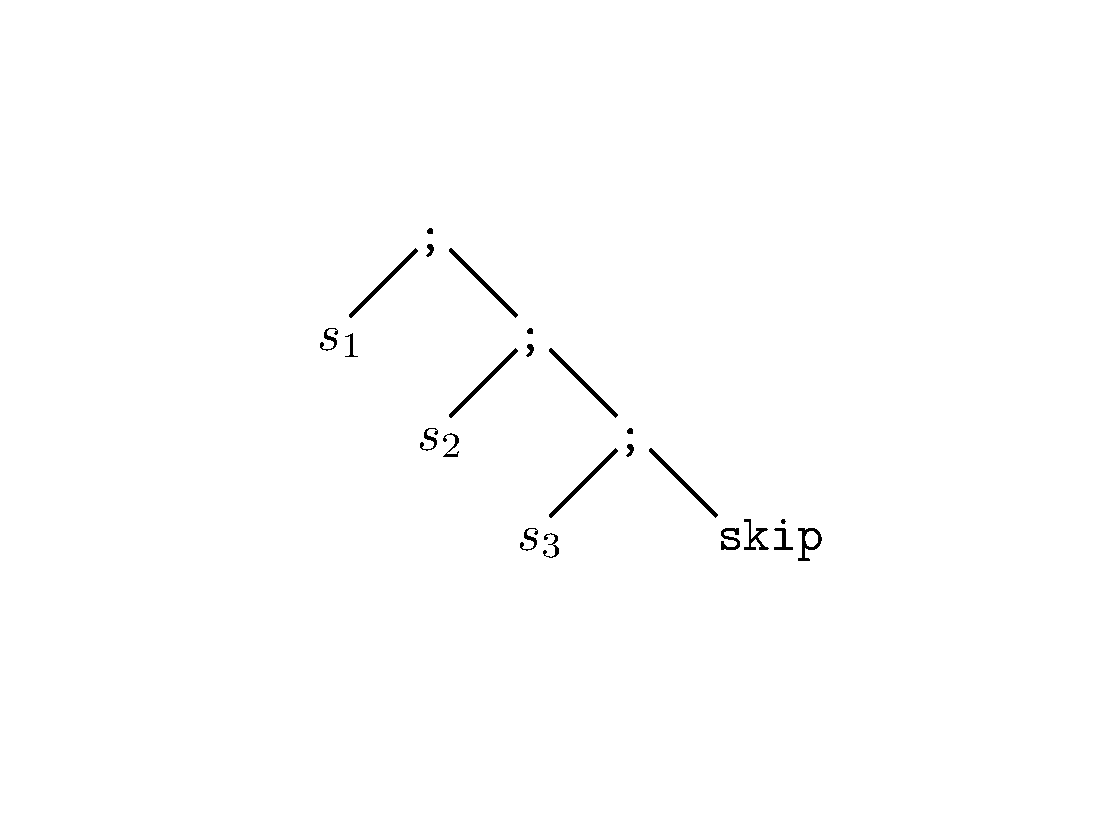
\includegraphics[trim={3cm 3cm 3cm 3cm}, clip, width=6cm]{graphics/rightAssocSkip}
\end{exmp}
These assumptions highly simplify reasoning about statements.

    % if then else???
    
    \subsection{Program State}
    \label{ssec:program-state}
    The set of program states is defined as $\setProgramState = \setHeap \times \setStack$ where
\begin{align*}
	S & \in \setStack      &  & ::= E \cdot S ~|~ \nil                               \\
	E & \in \setStackEntry &  & =~~ \setVarEnv \times \setDFootprint \times \setStmt
\end{align*}

% A program state of \svlidf consists of a single heap and a stack.
Each stack frame has an environment $\setVarEnv$ for local variables, tracks a set of accessible fields $\setDFootprint$ and stores a continuation $\setStmt$.
Stack frames will be introduced by method calls, but also by dedicated scopes as used by the $\ttt{hold}$ statement.

\begin{comment}
REQUIRED?
\begin{definition}[Topmost Stack Entry]
    Let $\topmost : \setStack \rightharpoonup \setStackEntry$ be defined as
    \begin{align*}
    &\topmost(E \cdot S) = E\\
    &\topmost(\nil) \quad\textit{ undefined}
    \end{align*}
\end{definition}

Program states with scheduled statement $s$ are defined as
\begin{displaymath}
\setProgramState_s ~\defeq~ \setHeap ~\times~ \{~~ (\rho, A_d, s) \cdot S ~~|~~ \rho \in \setVarEnv,~ A_d \in \setDFootprint,~ S \in \setStack ~~\}
\end{displaymath}
\end{comment}
        
    \subsection{Formula Semantics}
    \label{ssec:formula-semantics}
    

\begin{figure}
    \boxed{\evale {e} {v}}
    
\begin{mathpar}
    \inferrule* [right=EEVar]
    {~}
    {\evale {x} {\rho(x)}}
    
    \inferrule* [right=EEValue]
    {~}
    {\evale {v} {v}}
    
    \inferrule* [right=EEAcc]
    {\evale {e} {o}}
    {\evale {e.f} {H(o)(f)}}
\end{mathpar}
    \caption{\svlidf: Evaluating Expressions}
\end{figure}

\begin{figure}
    \boxed{\evalphi \phi}
    \input{data/autogen/dynamicFormula}

\begin{mathpar}
    \inferrule* [Right=EASepOp]
    {
        A_1 = A \backslash A_2 \\
        \evalphix H \rho {A_1} {\phi_1} \\
        \evalphix H \rho {A_2} {\phi_2}
    }
    {\evalphi {\phiCons {$\phi_1$} {$\phi_2$}}}
\end{mathpar}
    \caption{\svlidf: Evaluating Formulas}
\end{figure}

\begin{figure}[h]
    \begin{align*}
    A_d    & \in \setDFootprint &  & =~~ \PP^{\setLoc \times \setFieldName} 
    \end{align*}
    \boxed{\dynamicFP {H} {\rho} {\phi} = A_d}
    
\begin{align*}
	 & \dynamicFP {H} {\rho} {\phiTrue}                     &  & = \emptyset                                                          \\
	 & \dynamicFP {H} {\rho} {\phiEq{$e_1$}{$e_2$}}         &  & = \emptyset                                                          \\
	 & \dynamicFP {H} {\rho} {\phiNeq{$e_1$}{$e_2$}}        &  & = \emptyset                                                          \\
	 & \dynamicFP {H} {\rho} {\phiAcc{$x$}{$f$}}            &  & = \{\langle o,f \rangle\} \text{ where } \evale x o                  \\
	 & \dynamicFP {H} {\rho} {\phiCons{$\phi_1$}{$\phi_2$}} &  & = \dynamicFP {H} {\rho} {\phi_1} \cup \dynamicFP {H} {\rho} {\phi_2}
\end{align*}

What about undefinedness of acc case? Guess: propagates to undefinedness of small-step rule => covered by soundness
    \caption{\svlidf: Dynamic Footprint}
    \label{fig:dfp}
\end{figure}

\begin{figure}
    \boxed{\evalphiGen {\pi} {\phi}}
    \begin{mathpar}
        \inferrule* [Right=EvalFrm]
        {
            \evalphi {\phi}
        }
        {
            \evalgphiGen{(H, (\rho, A, s) \cdot S)}{\phi}
        }
    \end{mathpar}
    \caption{\svlidf: Evaluating Formulas}
\end{figure}
    
        \subsubsection{Framing}
        \label{sssec:framing}
        The integral advantage of IDF is the ability to use heap-dependent predicates in formulas.
In case of \svlidf, this means that fields may be used in formulas.
As illustrated in section \ref{ssec:implicit-dynamic-frames}, a formula must contain accessibility-predicates for all fields it references.
Otherwise, one cannot reason safely about writes to the heap.
% Accessibility-predicates are explicitly tracked as part of formulas and thus reflect a static
In this section we will formalize the requirements 

To guarantee safe reasoning about such formulas, they must contain accessibility predicates for all locations they are referencing.



%% other stuff
For future reference, we give further (non-syntactic) definitions:
\begin{figure}[h]
    \begin{align*}
    	A_s    & \in \setSFootprint &  & =~~ \PP^{\setExpr \times \setFieldName} \\
    	A_d    & \in \setDFootprint &  & =~~ \PP^{\setLoc \times \setFieldName} 
    \end{align*}
    \caption{\svlidf: Further Definitions}
\end{figure}

%An IDF assertion is self-framing if:
%For any state in which the assertion is true,
%it remains true if we replace the heap with any that agrees on the locations to which it requires permissions

\svlidf uses the concepts of implicit dynamic frames to ensure that a statement can only access memory locations (more specifically: fields) which it is guaranteed to have exclusive access to.
This is achieved by explicitly tracking access tokens $\phiAcc{\textit{<expression>}}{\textit{<field>}}$ as part of formulas throughout the entire program during verification.
    
The Hoare rules of \svlidf also make sure that access is never duplicated within or across stack frames, effectively ruling out concurrent access to any field during runtime.

Implicit dynamic frames also allows static reasoning about the values of fields during verification, i.e. as part of verification formulas.
In order to guarantee that such formulas always reflect the program state (preservation), formulas mentioning a certain field must also contain the access token to that very field:
\begin{definition}[Self-Framing]
    A formula is \textbf{self-framing} if it contains access to all fields it mentions.
\end{definition}

% EXAMPLE of verification without self-framing.

\begin{figure}
    \boxed{A_s \sfrme e}
    
\input{data/autogen/staticExpression}
    \caption{\svlidf: Framing Expressions}
\end{figure}

\begin{figure}
    \boxed{A_s \sfrmphi \phi}
    
\input{data/autogen/staticFormula}
    \caption{\svlidf: Framing Formulas}
\end{figure}

We omit the emptyset... 

\begin{definition}[Self-Framing Formula]
    A formula $\phi$ is \textbf{self-framing} iff
    \begin{displaymath}
    \sfrmphi \phi
    \end{displaymath}
    Let $\setFormulaB \subseteq \setFormulaA$ be the set of \textbf{self-framing and satisfiable} formulas.
\end{definition}


\svl will thus only consider method contracts using self-framing and satisfiable formulas well-formed (see section \ref{sec:well-formedness}).

\begin{figure}
    \boxed{\staticFP {\phi} = A_s}
    \begin{align*}
	 & \staticFP {\phiTrue}                       &  & = \emptyset                                  \\
	 & \staticFP {\phiEq {$e_1$} {$e_2$}}         &  & = \emptyset                                  \\
	 & \staticFP {\phiNeq {$e_1$} {$e_2$}}        &  & = \emptyset                                  \\
	 & \staticFP {\phiAcc {$e$} {$f$}}            &  & = \{\langle e,f \rangle\}                                  \\
	 & \staticFP {\phiCons {$\phi_1$} {$\phi_2$}} &  & = \staticFP {\phi_1} \cup \staticFP {\phi_2}
\end{align*}


    \caption{\svlidf: Static Footprint}
\end{figure}

%IS conservative approximation of formulas that are dynamically framed (not possible precisely anyway!)
        
        % RULES arising from this semantics!!! e.g. implication:
        % - a * b => a
        % - a !=> a * a
    
    \subsection{Static Semantics}
    \label{sec:static-semantics}
    % AXIOMATIC
The static semantics of \svl consist of typing rules and a Hoare calculus making use of those typing rules.
All the rules are implicitly parameterized over some program $p \in \setProgram$, necessary for example to extract the type of a field in the following typing rules.

\begin{figure}[h]
    \boxed{\sType{\Gamma}{e}{T}}
    %\input{data/autogen/staticTypeExpression}
\input{data/autogenx/staticTypeExpression}
    \caption{\svl: Static Typing of Expressions}
\end{figure}

\begin{figure}[h!]
    \boxed{\thoare {\Gamma} {\phi_{pre}} {\overline{s}} {\phi_{post}}}
    \input{data/autogen/staticSemantics}
    \caption{\svl: Hoare Calculus} 
\end{figure}


%% FRAMING
%% Inductive Semantics.sfrme
\begin{mathpar}
\inferrule* [Right=WFVar]
{
    ~
}
{
    {A} \sfrme {\ex{${x}$}}
}
\end{mathpar}

\begin{mathpar}
\inferrule* [Right=WFValue]
{
    ~
}
{
    {A} \sfrme {\ev{${v}$}}
}
\end{mathpar}

\begin{mathpar}
\inferrule* [Right=WFField]
{
    {({e}, {f})} \in {A} \\
    {A} \sfrme {e}
}
{
    {A} \sfrme {\edot{${e}$}{${f}$}}
}
\end{mathpar}


        
        \subsubsection{Typing}
        \label{sssec:typing}
        
\begin{figure}[h]
    \boxed{\sType{\Gamma}{e}{T}}
    %\input{data/autogen/staticTypeExpression}
\input{data/autogenx/staticTypeExpression}
    \caption{\svl: Static Typing of Expressions}
\end{figure}
    
        \subsubsection{Verification}
        \label{sssec:verification}
        
\begin{figure}[h!]
    \boxed{\thoare {\Gamma} {\phi_{pre}} {s} {\phi_{post}}}
    \input{data/autogen/staticSemantics}
    \caption{\svl: Hoare Logic} 
\end{figure}

Let $\wsp : \setStmt \rightarrow \PP(\setProgramState)$ be defined as
\newcommand{\tempDefPS}{\{~ \pi \in \setProgramState_s ~|~ \exists \phi_1, \phi_2 \in \setFormula,\, \Gamma \in \setTypeEnv.~ \thoare{\Gamma}{\phi_1}{s}{\phi_2} ~~\wedge~~ \evalphiGen{\pi}{\phi_1} ~\}}
\begin{flalign*}
	 & \wsp(s)                 & =~ & \tempDefPS       & ~ \\
	 & \wsp(s) & =~ &
     \begin{cases}
     	\setProgramState_s                                                                                  & \text{if~} s = \sAlloc{$x$}{$C$}            \\
     	\{~ \pi \in \setProgramState_s ~|~ \evalphiGen{\pi}{\phiAcc{$x$}{$f$}} ~\}                          & \text{if~} s = \sFieldAssign{$x$}{$f$}{$y$} \\
     	\{~ \pi \in \setProgramState_s ~|~ \evalphiGen{\pi}{\accFor{$e$}} ~\}                               & \text{if~} s = \sVarAssign{$x$}{$e$}        \\
     	\setProgramState_s                                                                                  & \text{if~} s = \sReturn{$x$}                \\
     	\{~ \pi \in \setProgramState_s ~|~ \evalphiGen{\pi}{\phiCons{\phiNeq{$y$}{\enull}}{\mpre{$m$}}} ~\} & \text{if~} s = \sCall{$x$}{$y$}{$m$}{$z$}   \\
     	\{~ \pi \in \setProgramState_s ~|~ \evalphiGen{\pi}{$\phi$} ~\}                                     & \text{if~} s = \sAssert{$\phi$}             \\
     	\{~ \pi \in \setProgramState_s ~|~ \evalphiGen{\pi}{$\phi$} ~\}                                     & \text{if~} s = \sRelease{$\phi$}
     \end{cases}
       & ~ \\ 
\end{flalign*}
    
    \subsection{Well-Formedness}
    \label{sec:well-formedness}
    Apart from checking method contracts, a verifier or compiler may enforce further rules before accepting a program as “well formed”.
For \svlidf we give the rules formalized in figure \ref{fig:idf-wf}.

\begin{figure}[h]
    
\begin{mathpar}
\inferrule* [Right=OkProgram]
{
\overline{cls_i \OK} \\
\thoare {~} {\phiTrue} {s} {\phi}
}
{(\overline{cls_i}~s) \OK}
\end{mathpar}

\begin{mathpar}
\inferrule* [Right=OkClass]
{
\text{unique $field$-names} \\
\text{unique $method$-names} \\
\overline{method_i \OKinC}
}
{(\class {$C$} {$\overline{field_i}$} {$\overline{method_i}$}) \OK}
\end{mathpar}

\begin{mathpar}
\inferrule* [Right=OkMethod]
{
    \thoare {x : T_x, \ethis : C, \eresult : T_m} {\phi_1} {s} {\phi_2} \\\\
    \FV(\phi_1) \subseteq \{ x, \ethis \} \\
    \FV(\phi_2) \subseteq \{ x, \ethis, \eresult \} \\\\
    \sfrmphi \phi_1 \\
    \sfrmphi \phi_2 \\
    \neg \writesTo(s, x)
}
{(\method {$T_m$} {$m$} {$T_x$} {$x$} {\contract {$\phi_1$} {$\phi_2$}} {$s$}) \OKinC}
\end{mathpar}
    \caption{\svlidf: Well-Formedness}
    \label{fig:idf-wf}
\end{figure}

%% OkMethod
The premises of $\tset{OkMethod}$ make sure that reasoning about calls is sound.
As expected, the method contract is checked, while also making sure that it contains self-framing formulas.
Furthermore, the free variables are restricted to those occurring in the method signature.
The following example illustrates why this is necessary.

%% example
\begin{example}{Leaking Postcondition}
\begin{lstlisting}
int identity(int a)
    requires true;
    ensures  (b = 3);
{
    int b;
    b = 3;
    return a;
}
\end{lstlisting}
While the method passes static verification, it could lead to unsound proofs.
Note how \tset{HCall} forwards the postcondition after replacing known variables with their counterparts.
\phiEq{b}{3} is unaffected by this replacement, ending up in the postcondition of the call statement.

Should the call site also know a variable \ttt{b}, then \phiEq{b}{3} will most likely not reflect the state of that variable.
\end{example}

For similar reasons, we prevent writes to the method's parameter.
Changes to the parameter would otherwise end up in the postcondition which is forwarded to the call site.
Information about the formal parameter is then reflected back on the variable passed as actual parameter for the method call.
However, since parameters are passed by value, this information would be false -- the actual parameter will have the same value before and after the method call.

    
    \subsection{Dynamic Semantics}
    \label{ssec:dynamic-semantics}
    % MENTION that most of that stuff is completely redundant if soundness holds - and only used to prove just that!
The small-step semantics $\sstep{\cdot}{\cdot} : \setProgramState \rightharpoonup \setProgramState$ of \svlidf are defined inductively in figure \ref{fig:svl-sem-dyn-sstep}.
Note that right-associativity of \ttt{;} and termination of sequences with $\sSkip$ (see section \ref{sec:syntax}) obviates the need for dedicated sequence rules.

Using inductive rules to define a partial function, we have to make sure that at most one result is deducible for every input.
\begin{lemma}[$\sstep{\cdot}{\cdot}$ Well-Defined]
    The small-step semantics of \svlidf is well-defined.
\end{lemma}
\begin{proof}
    For $\sstep{\cdot}{\cdot}$ to be well-defined, at most one result can be deducible per input.
    The rules in figure \ref{fig:svl-sem-dyn-sstep} are syntax directed, so we can focus on individual rules when checking for determinism.
    This can be done by looking at the source of all variables used to construct return values (i.e. the variables used on the right hand side of $\sstep{}{}$ in the conclusion).
    All those variables must either be drawn directly from the input or be uniquely specified using premises.
    
    \tset{\gradT SsSkip}
    $H, \rho, A, s, S$ are directly drawn from the input.
    
    \tset{\gradT SsFieldAssign}
    $\rho, A, s, S$ are directly drawn from the input, $H'$ is defined using premises and depends on the uniqueness of $H, o, f, v_y$.
    These are drawn from input or are result of expression evaluation which is deterministic.
    
    The same approach can be used for all remaining rules.
\end{proof}

\begin{figure}
    \boxed{\sstep{\pi}{\pi}}
    %\input{data/autogen/dynamicSemantics}
\input{data/autogenx/dynamicSemantics}
    \caption{\svlidf: Small-Step Semantics}
    \label{fig:svl-sem-dyn-sstep}
\end{figure}


% Again, the semantics is implicitly parameterized over some program $p$.
    
    \subsection{Soundness}
    % invariants?

\section{Gradual Syntax}
\label{sec:cs-gradual-formulas}
%% intro
The first step of deriving \gvlidf is defining its modified syntax.
As motivated in section \ref{sec:gradual-formulas} we first extend the formula syntax, afterwards everything that depends on it.

%% formula syntax & concretization
In our design of gradual formulas we aim for “bounded unknown” formulas as introduced in section \ref{ssec:wildcard-with-upper}, however with separating conjunction as a connective:
\begin{description}
    \item[Syntax] 
    \begin{flalign*}
    	 & \grad{\phi} \quad::=\quad \phi ~|~ \withqm{\phi} &
    \end{flalign*}
    We pose $\qm \defeq \withqm{\phiTrue}$.
    
    % ONLY used for normal form
    %We call formulas containing $\qm$ “partially-unknown” (i.e. a gradual formula is either static or partially-unknown).  
    
    \item[Concretization]
    \begin{flalign*}
    & \gamma(\phi) = \{~ \phi ~\}                                                         & ~ \\
    & \gamma(\withqm{\phi}) = \{~ \phi' \in \setFormulaB ~|~ \phiImplies{\phi'}{\phi} ~\} &
    \end{flalign*}
    
    Note that we do not require the static part of $\withqm{\phi}$ to be self-framing.
    On the contrary, we want concretizations to be able to provide framing for an otherwise unframed formula.
    (We decided to put $\qm$ in front of the static part to emphasize that fact.)
    This allows programmers to resort to gradual formulas when being uncertain or indifferent about the concrete framing of a heap-dependent formula.
    \begin{example}{Unknown Framing}
        The programmer may want to express $\phiEq{a.name}{b.name}$, but is indifferent about whether \ttt{a} and \ttt{b} alias or not.
        As shown in section \ref{sssec:regular-conjunction}, both options are not expressible at the same time using a static formula.
        Fortunately, $\qm$ can be used to frame the formula, covering both alternatives:
        \begin{flalign*}
        	\phiCons{\phiCons{\phiAcc{a}{name}}{\phiAcc{b}{name}}}{\phiEq{a.name}{b.name}} & \in \gamma(\withqm{\phiEq{a.name}{b.name}}) & ~~~~~ \\
        	\phiCons{\phiCons{\phiEq{a}{b}}{\phiAcc{b}{name}}}{\phiEq{b.name}{b.name}}      & \in \gamma(\withqm{\phiEq{a.name}{b.name}}) &
        \end{flalign*}
    \end{example}
    
    \item[Static Knowledge Extraction]~\\
    We define a helper function $\static{} : \setGFormula \rightarrow \setFormula$ that extracts the static part of a gradual formula as follows:
    \begin{alignat*}{2}
    	 & \static{$\phi$}          &~= \phi & ~ \\
    	 & \static{$\withqm{\phi}$} &~= \phi &
    \end{alignat*}
\end{description}

%% gradual syntax
We want to only allow gradual formulas in method contracts, resulting in the gradual syntax shown in figure \ref{fig:gidf-syntax}.
\begin{figure}[h]
    \begin{align*}
	\grad{program}  & \in \setGProgram  &  & ::= \ttt{$\overline{\grad{cls}}$~$\grad{s}$}                         \\
	\grad{cls}      & \in \setGClass    &  & ::= \class {$C$} {$\overline{field}$} {$\overline{\grad{method}}$}   \\
	\grad{method}   & \in \setGMethod   &  & ::= \method {$T$} {$m$} {$T$} {$x$} {$\grad{contract}$} {$\grad{s}$} \\
	\grad{contract} & \in \setGContract &  & ::= \contract{$\grad{\phi}$}{$\grad{\phi}$}                          \\
	\grad{\phi}     & \in \setGFormula  &  & ::= \phi ~|~ \withqm{\phi}
\end{align*}
    \caption{\gvlidf: Syntax}
    \label{fig:gidf-syntax}
\end{figure}
Note how the small change propagates throughout other constructs, all the way up to gradual programs.
However, the change has no direct impact on statement syntax, allowing us to define $\setGStmt \defeq \setStmt$ and therefore $\setGProgramState \defeq \setProgramState$.
Note that we also have not decorated $s$ in figure \ref{fig:gidf-syntax} although it is formally drawn from $\setGStmt$.
There is no point in decorating statements or program state in of \gvlidf.
However, note that static and dynamic semantics of the call statement $\sCall {$x$} {$y$} {$m$} {$z$}$ will still have to be lifted as $m$ now references a gradual method contract (see section \ref{sec:gradual-statements} for detailed discussion).


    \subsection{Extension: Statements}
    \label{ssec:extension--statements}
    
%% method contract extension
In \gvl we want the programmer to specify gradual method contracts.
Therefore we extend their syntax as follows.
\begin{align*}
\grad{contract} & \in \setGContract   &  & ::= \ttt{requires $\grad{\phi}$;~ensures $\grad{\phi}$;}
\end{align*}

%%% propagation
This extension is propagated to method declarations (now accepting gradual contracts but not changing otherwise), yielding $\setGMethod$.
Carrying on with the same logic, we get an extended set of class definitions $\setGClass$ and finally an extended set of programs $\setGProgram$.
Again, note that the only syntactical difference is the acceptance of gradual formulas in method contracts.

%% statements
We see no motive to extend the syntax of statements themselves and define $\setGStmt = \setStmt$.
As postulated in section \ref{sec:gradual-statements}, the call statement hides away gradualized syntax by referencing a method with gradual contract.
This becomes obvious when looking at its static or dynamic semantics (see \tset{HCall} and \tset{ESCall???}/\tset{ESCallFinish}) where the method name is effectively dereferenced.
% SO we will remember that when lifting stuff...

    \subsection{Extension: Program State}
    $\setGProgramState = \setProgramState$

\section{Gradual Static Semantics}
\label{sec:gradualize-hoare-rules}
Figure \ref{fig:gvl-sem-stat-hoare} shows a deterministic lifting of the Hoare logic (figure \ref{fig:svl-sem-stat-hoare}).
It uses a number of helper functions that we define in section \ref{ssec:lifted-helper-functions}.
\begin{figure}[h!]
    \boxed{\dgthoare {\Gamma} {\grad{\phi_{pre}}} {s} {\grad{\phi_{post}}}}
    \begin{mathpar}
    \inferrule* [right=\dgradT HSkip]
    {
        ~
    }
    {
        \dgthoare {\Gamma} {\grad{\phi}} {{\sSkip}} {\grad{\phi}}
    }
    
    \inferrule* [Right=\dgradT HAlloc]
    {
        {\wo {\grad{\phi}} {x}} = \grad{\phi'}\\
        \sType {\Gamma} {\ex{${x}$}} {{C}} \\
        {\fields{C}} = {{\overline{\field{$T$}{$f$}}}}
    }
    {
        \dgthoare {\Gamma} {\grad{\phi}} {{\sAlloc {${x}$} {${C}$}}} {\gphiCons{$\grad{\phi'}$}{${\gphiCons{${\phiNeq {${\ex{${x}$}}$} {${\ev{${\enull}$}}$}}$}{${\overline{\gphiCons{\phiAcc {$x$} {$f_i$}}{\phiEq {\edot {$x$} {$f_i$}} {\defaultValue {$T_i$}} }}}$}}$}}
    }
    
    \inferrule* [Right=\dgradT HFieldAssign]
    {
        \wo {\grad{\phi}} {\phiAcc{$x$}{$f$}} = \grad{\phi'}\\
        \sType {\Gamma} {\ex{${x}$}} {{C}} \\
        \sType {\Gamma} {\ex{${y}$}} {T} \\
        \vdash {C}.{f} : {T}
    }
    {
        \dgthoare {\Gamma} {\grad{\phi}} {{\sFieldAssign {${x}$} {${f}$} {${y}$}}} {\gphiCons{$\grad{\phi'}$}{${\gphiCons{${\phiAcc {${\ex{${x}$}}$} {${f}$}}$}{${\gphiCons{${\phiNeq {${\ex{${x}$}}$} {${\ev{${\enull}$}}$}}$}{${\ensuremath{{\phiEq {${\edot{${\ex{${x}$}}$}{${f}$}}$} {${\ex{${y}$}}$}}}}$}}$}}$}}
    }
    
    \inferrule* [Right=\dgradT HVarAssign]
    {
        \gphiImplies{\grad{\phi}} {\accFor {{e}}}\\
        {\wo {\grad{\phi}} {x}} = \grad{\phi'}\\
        {x} \not \in {\FV({e})} \\
        \sType {\Gamma} {\ex{${x}$}} {T} \\
        \sType {\Gamma} {e} {T}
    }
    {
        \dgthoare {\Gamma} {\grad{\phi}} {{\sVarAssign {${x}$} {${e}$}}} {\gphiCons{$\grad{\phi'}$}{${\ensuremath{{\phiEq {${\ex{${x}$}}$} {${e}$}}}}$}}
    }
    
    \inferrule* [Right=\dgradT HReturn]
    {
        {\wo {\grad{\phi}} {\eresult}} = \grad{\phi'}\\
        \sType {\Gamma} {\ex{${x}$}} {T} \\
        \sType {\Gamma} {\ex{${\eresult}$}} {T}
    }
    {
        \dgthoare {\Gamma} {\grad{\phi}} {{\sReturn {${x}$}}} {\gphiCons{$\grad{\phi'}$}{${\ensuremath{{\phiEq {${\ex{${\eresult}$}}$} {${\ex{${x}$}}$}}}}$}}
    }
    
    \inferrule* [Right=\dgradT HCall]
    {
        \wo {\wo {\grad{\phi}} {x}} {\grad{\phi_p}} = \grad{\phi'}\\
        \sType {\Gamma} {\ex{${y}$}} {{C}} \\
        {\mmethod{{C}, {m}}} = {{\method {${T_r}$} {${m}$} {${T_p}$} {${z}$} {${\contract {$\grad{\phi_{pre}}$} {$\grad{\phi_{post}}$}}$} {${\usc}$}}} \\
        \sType {\Gamma} {\ex{${x}$}} {T_r} \\
        \sType {\Gamma} {\ex{${z'}$}} {T_p} \\
        \gphiImplies{\grad{\phi}}{\gphiCons{${\phiNeq {${\ex{${y}$}}$} {${\ev{${\enull}$}}$}}$}{$\grad{\phi_p}$}} \\
        x \neq y \wedge x \neq z' \\
        \grad{\phi_p} = {\grad{\phi_{pre}}[{y}, {z'} / {\ethis}, {{z}}]} \\
        \grad{\phi_q} = {\grad{\phi_{post}}[{y}, {z'}, {x} / {\ethis}, {{z}}, {\eresult}]}
    }
    {
        \dgthoare {\Gamma} {\grad{\phi}} {{\sCall {${x}$} {${y}$} {${m}$} {${z'}$}}} {\gphiCons{$\grad{\phi'}$}{$\grad{\phi_q}$}}
    }
    
    \inferrule* [right=\dgradT HAssert]
    {
        \gphiImpliesEv{\grad{\phi}}{\phi_a}{\grad{\phi'}}
    }
    {
        \dgthoare {\Gamma} {\grad{\phi}} {{\sAssert {${\phi_a}$}}} {\grad{\phi'}}
    }
    
    \inferrule* [Right=\dgradT HRelease]
    {
        \gphiImpliesEv{\grad{\phi}}{\phi_r}{\grad{\phi'}}\\
        {\wo {\grad{\phi'}} {\phi_r}} = \grad{\phi''}
    }
    {
        \dgthoare {\Gamma} {\grad{\phi}} {{\sRelease {${\phi_r}$}}} {\grad{\phi''}}
    }
    
    \inferrule* [Right=\dgradT HDeclare]
    {
        {x} \not\in \dom{\Gamma} \\
        {x} \not \in {\FV(\grad{\phi})} \\
        \dgthoare {{\Gamma}, {x} : {T}} {\gphiCons{${\phiEq {${\ex{${x}$}}$} {${\ev{${\defaultValue{${T}$}}$}}$}}$}{$\grad{\phi}$}} {s} {\grad{\phi'}}
    }
    {
        \dgthoare {\Gamma} {\grad{\phi}} {\sSeq{\sDeclare {${T}$} {${x}$}}{$s$}} {\grad{\phi'}}
    }
    
    \inferrule* [Right=\dgradT HHold]
    {
        \sfrmphi {\phi} \\
        \gphiImpliesEv{\grad{\phi_f}}{\phi}{\grad{\phi_f'}}\\
        \wo {\grad{\phi_f'}} {\phi} = \grad{\phi_r}\\
        \wo {\wo {\grad{\phi_f'}} {\static{$\grad{\phi_r}$}}}{(\FV(\grad{\phi_f'}) \backslash \FV(\phi))} = \grad{\phi'}\\
        \mods(s) \cap \FV(\phi) = \emptyset \\
        \dgthoare {\Gamma} {\grad{\phi_r}} {s} {\grad {\phi_r'}}
    }
    {
        \dgthoare {\Gamma} {\grad{\phi_f}} {{\sHold {${\phi}$} {$s$}}} {\gphiCons{$\grad{\phi_r'}$}{$\grad{\phi'}$}}
    }
    
    \inferrule* [Right=\dgradT HSeq]
    {
        \dgthoare {\Gamma} {\grad{\phi_p}} {s_1} {\grad{\phi_q}} \\
        \dgthoare {\Gamma} {\grad{\phi_q}} {s_2} {\grad{\phi_r}}
    }
    {
        \dgthoare {\Gamma} {\grad{\phi_p}} {\sSeq{$s_1$}{$s_2$}} {\grad{\phi_r}}
    }
\end{mathpar}





% Let $\gsc$ behave like $\hsc$ if first operand is static - otherwise its regular concatenation.




    \caption{\gvl: Gradual Hoare Logic} 
    \label{fig:gvl-sem-stat-hoare}
\end{figure}

\begin{lemma}[\gvlidf: Sound Deterministic Lifting of Hoare Logic]
    The inductive definition we give induces a well-defined partial function.
    This function is a sound deterministic lifting (see \ref{ssec:the-deterministic-approach}) of the Hoare logic of \svlidf defined in section \ref{sec:static-semantics}.
\end{lemma}

A sound predicate lifting $\gtHoare{\cdot}{\cdot}{\cdot}{\cdot}$ can be derived using lemma \ref{lem:det2grad}.

\section{Gradual Dynamic Semantics}
\label{sec:gradual-dyn--semantics}
The call statement is the only statement that is affected by the introduction of gradual formulas.
As we do not want the semantics of any of the other statements to change, we only have to adjust the rules for calls.
Figure \ref{fig:gvl-sem-dyn-sstep} shows those rules.
\begin{figure}
    \boxed{\gsstep{\pi}{\pi}}
    % Inductive Semantics.dynSem
\begin{mathpar}
\inferrule* [Right=\gradT ESCall]
{
    \evalex {H} {\rho} {\ex{${y}$}} {{o}} \\
    \evalex {H} {\rho} {\ex{${z}$}} {v} \\
    {H(o)} = {{\langle{C}, {\usc}\rangle}} \\
    {\mmethod{{C}, {m}}} = {{\method {${T_r}$} {${m}$} {${T}$} {${w}$} {${\contract {$\grad{\phi}$} {${\usc}$}}$} {$\grad{r}$}}} \\
    {\rho'} = {[{\eresult} \mapsto {\defaultValue{${T_r}$}}, {\ethis} \mapsto {{o}}, {{w}} \mapsto {v}]} \\
    \evalgphiGen {H, \rho', A} {\grad{\phi}} \\
    {A'} = {
    \begin{cases}
    	\dynamicFP {H} {\rho'} {\grad{\phi}} & \textit{if } \grad{\phi} \in \setFormula \\
    	A                                    & \textit{otherwise}
    \end{cases}}
}
{
    \sstep {\langle{H}, {{\langle{{\rho}, {A}}, {\sSeq{${\sCall {${x}$} {${y}$} {${m}$} {${z}$}}$}{$s$}}\rangle} \cdot {S}}\rangle} {\langle{H}, {{\langle{{\rho'}, {A'}}, \grad{r}\rangle} \cdot {{\langle{{\rho}, {{A} \backslash {A'}}}, {\sSeq{${\sCall {${x}$} {${y}$} {${m}$} {${z}$}}$}{$s$}}\rangle} \cdot {S}}}\rangle}
}

\inferrule* [Right=\gradT ESCallFinish]
{
    \evalex {H} {\rho} {\ex{${y}$}} {{o}} \\
    {H(o)} = {{\langle{C}, {\usc}\rangle}} \\
    {\mpost{{C}, {m}}} = {\grad{\phi}} \\
    \evalgphiGen {H, \rho', A'} {\grad{\phi}} \\
    \evalex {H} {\rho'} {\ex{${\eresult}$}} {v_r}
}
{
    \sstep {\langle{H}, {{\langle{{\rho'}, {A'}}, {\sSkip}\rangle} \cdot {{\langle{{\rho}, {A}}, {\sSeq{${\sCall {${x}$} {${y}$} {${m}$} {${z}$}}$}{$s$}}\rangle} \cdot {S}}}\rangle} {\langle{H}, {{\langle{{{\rho}[{x} \mapsto {v_r}]}, {{A} \cup {A'}}}, s\rangle} \cdot {S}}\rangle}
}
\end{mathpar}


    \caption{\gvlidf: Small-Step Semantics for Method Call}
    \label{fig:gvl-sem-dyn-sstep}
\end{figure}
For all other statements $\gsstep{\cdot}{\cdot}$ is identical to $\sstep{\cdot}{\cdot}$ (see figure \ref{fig:svl-sem-dyn-sstep}).

Furthermore, we design $\gsstep{\cdot}{\cdot}$ to be total.
We extend the set of final states $\setGProgramStateFin$ with a designated exceptional state $\pi_{EX}$, representing dynamic verification failure.
If no other derivation exists, we map to this state.

\begin{lemma}[$\gsstep{\cdot}{\cdot}$ Well-Defined]
    The small-step semantics of \gvlidf is well-defined.
\end{lemma}
\begin{proof}
    For $\gsstep{\cdot}{\cdot}$ to be well-defined, the inductive rules may allow deducing at most one return value for every input.
    For the most part, this is the case due to $\sstep{\cdot}{\cdot}$ being well-defined (see lemma \ref{lemma:ss-wd}).
    We show that the same is true for adjustments made in figure \ref{fig:gvl-sem-dyn-sstep}.
    Note the adjustments do not change the fact that the inductive rules are syntax-directed.
    
    Rule \tset{\gradT SsCall} is deterministic:
    $H, \rho, A, x, y, m, z, s, S$ are forwarded from the input, $\rho', A', r$ are uniquely determined by the premises.
    
    Rule \tset{\gradT SsCallFinish} is deterministic:
    $H, \rho, x, A, A', s, S$ are forwarded from the input, $v_r$ is uniquely determined by the premises.
\end{proof}

\begin{lemma}[\gvlidf: Sound Lifting of Small-Step-Semantics]
    The lifting we propose is sound as defined in section \ref{sssec:lifting-partial-functions}.
\end{lemma}
\begin{proof}
    For the rules copied from $\sstep{\cdot}{\cdot}$, the rules are trivially satisfied as there is no difference between gradual and non-gradual statements.
    Precision is only meaningful for call statements:

    \begin{description}
        \item[\tset{\gradT SsCall}]~
        \begin{description}
            \item[Introduction]~\\
            For static precondition, \tset{\gradT SsCall} is identical to \tset{SsCall}.
            
            \item[Monotonicity]~\\
            Reducing the precision of the precondition results in all permissions being passed to the topmost stack frame.
            Having more permissions than before cannot introduce runtime failures.
            Succeeding executions will thus be observationally identical after reducing precision.
        \end{description}
        
        \item[\tset{\gradT SsCallFinish}]~
        \begin{description}
            \item[Introduction]~\\
            For static postcondition, \tset{\gradT SsCallFinish} is identical to \tset{SsCallFinish}.
            
            \item[Monotonicity]~\\
            The return value of \tset{\gradT SsCallFinish} is independent of the postcondition thus monotonic w.r.t. to it.
            In terms of definedness, reducing the precision of the postcondition cannot result in premises that were satisfied before to be unsatisfied.
        \end{description}
    \end{description}
\end{proof}
% thing with HSec
% Tapp usw...

% THIS IS WHERE THE SIMPLIFICATION AND ALL ITS REASONING COMES IN!


\chapter{Evaluation/Analysis}
\label{ch:evaluation-analysis}

> E:
with gradual typestates the same problem happened: as soon as the potential for unknown annotations was accepted, there was a “baseline cost” just to maintain the necessary infrastructure.
With simple gradual types, it’s almost nothing. With gradual effects, we’ve shown that it can boil down to very little (a thread-local variable with little overhead, see OOPSLA’15). 

% relationship LC and verification! which rules are derived by which, correspondence table

\section{Enhancing an Unverified Language}
\label{sec:enhancing-an-unverified}
%% intro
The approach we presented constructs a gradually verified language in terms of a statically verified one.
However, as the example in section \ref{ssec:argument-validation} motivates, gradual verification can also be seen as an extension of the dynamically verified setting.
The main drawbacks of dynamic verification (runtime overhead and potentially late error detection) would be counteracted by using static verification techniques where possible.
A gradual verifier will attempt to prove compliance with annotations (making runtime checks unnecessary) or may detect an inevitable violation of an annotation (detecting an error before the program is executed).
In this section, we will briefly describe how to turn a dynamically verified language into a gradually verified one.

%% dyn ver spectrum
To understand how to approach dynamically verified languages, we have to examine how they fit into the spectrum of a gradually verified one.
The static end is (by construction) the one where all formulas are static and the unknown formula “\qm” is never used.
In contrast, annotating $\qm$ everywhere corresponds to a system that solely relies on runtime checks.
One can further define that leaving out annotations (e.g. precondition, postcondition, or even both) corresponds to an annotation of $\qm$.
A dynamically verified language (say, Java) can be imitated using this process.
Given such a language, the steps are thus as follows:

%% steps
First one has to identify what the goal of a static verification system would be for the language at hand.
Common examples include race-condition avoidance or a no-throw guarantee.
One can then develop a sound Hoare logic that achieves that goal, including syntax extensions to the language that allow leveraging that Hoare logic.
Gradualization can be applied to that system, introducing $\qm$ as a “default formula”, which allows making all newly introduced syntax extensions optional again.
The syntax of the resulting gradually verified language should thus be a superset of the dynamically verified one.
Contracts that were before explicitly realized as runtime checks can now be removed and encoded using the extended syntax.


\chapter{Conclusion}
\label{ch:conclusion}
Gradual verification aims to overcome drawbacks of static or dynamic verification by seamlessly combining both approaches.
As a result, programmers can freely choose the amount of static annotations to provide and thus have complete control over the degree of static verification used.

In this work we have developed a procedure of deriving an imperative gradually verified programming language from a statically verified one.
We have done so by adapting the work on “Abstracting Gradual Typing” (AGT, \cite{garcia2016abstracting}) by Garcia, Clark and Tanter to the setting of program verification.
Therefore, we used the concepts of abstract interpretation to give a meaning to gradual formulas.
Furthermore we generalized their notion of gradual lifting and applied it to the semantics of the statically verified language.
We also developed the notion of deterministic lifting in order to overcome a number of practical issues related to predicate lifting and transitivity.
Note that we did not make use of their way of providing gradual dynamic semantics using “evidence”, see section \ref{sec:soundness-using-evidence} for discussion.

Finally, we illustrated our approach by gradualizing an imperative statically verified language using implicit dynamic frames to enable safe reasoning about shared mutable data structures.

%Recap, remind reader what big picture was.
%Briefly outline your thesis, motivation, problem, and proposed solution.





\section{Conceptual Nugget: Comparison/Implication to AGT!}

\section{Limitations}
\label{sec:limitations}

no shared access...

\section{Future Work}
\label{sec:future-work}
\subsection{Optimality Revised}%% optimality
After realizing that optimality of gradual liftings (or “consistent lifting”, as called in AGT \cite{garcia2016abstracting}) is an unnecessary restriction in the verification setting, we focused mainly on soundness of liftings.
Furthermore, we showed that our approach of obtaining a gradual Hoare logic using deterministic liftings does not result in an optimally lifted Hoare logic, even if the deterministic lifting was optimal (see example \ref{cex:opt-det2grad}).
We have also shown that a more expressive gradual syntax can reduce that problem, yet we have not formally proved that relationship.

Furthermore, it is unclear whether optimality/consistency as defined by AGT is even desirable under all circumstances:
\begin{example}{Optimality and Decidability}
    Consider a statement $s$ which is very hard to reason about (for instance, think of 300 Collatz sequence iterations).
    With the static Hoare logic, we assume that
    \begin{displaymath}
    \thoare{}{\phiEq{x}{10000}}{s}{\phiAnd{\ttt{1 <= x}}{\ttt{x <= 4}}}
    \end{displaymath}
    can be verified and that no stronger postcondition could be verified (due to limitations of the verifier).
    However, we know that \ttt{x} will have value 4 afterwards, i.e. the following Hoare triple is valid:
    \begin{displaymath}
    \hoare{\phiEq{x}{10000}}{s}{\phiEq{x}{4}}
    \end{displaymath}
    
    Using gradual verification, we want to overcome the limitations imposed by decidability and be able to deduce 
    \begin{displaymath}
    \gthoare{}{\withqmGen{\phiEq{x}{10000}}}{s}{\withqmGen{\phiEq{x}{4}}}
    \end{displaymath}
    or similar.
    However, an optimal gradual lifting is not able to deduce this fact, since there exists no instantiation of the postcondition for which a corresponding static judgment holds (since $\phiAnd{\ttt{1 <= x}}{\ttt{x <= 4}} \not \in \gamma(\withqmGen{\phiEq{x}{4}})$).
   
    Note that our approach using a deterministic gradual Hoare logic would work in this case:
    \begin{displaymath}
    \dgthoare{}{\withqmGen{\phiEq{x}{10000}}}{s}{\withqmGen{\phiAnd{\ttt{1 <= x}}{\ttt{x <= 4}}}}
    \end{displaymath}
    or a more imprecise postcondition must be deducible due to introduction, strength and monotonicity rules.
    Furthermore $\gphiImplies{\withqmGen{\phiAnd{\ttt{1 <= x}}{\ttt{x <= 4}}}}{\phiEq{x}{4}}$ holds (emitting a runtime check), such that 
    \begin{displaymath}
    \gthoare{}{\withqmGen{\phiEq{x}{10000}}}{s}{\phiEq{x}{4}}
    \end{displaymath}
    is deducible.
\end{example}

\begin{comment}
INTERESTING! Regarding “when does optimal det. lift. imply opt. pred. lift.”
For above example, the gradual formula syntax would have to provide a way of saying that there is NOT MORE knowledge about x hidden in ?.
This way, the gradual implication of x = 4 would (as expected) fail, as the optimal predicate would
\end{comment}

We conjecture that a notion of consistency that relies on semantically valid Hoare triples instead of statically deducible ones (Hoare logic) would solve this problem, yet it is unclear what the implications of this definition would be.
Most importantly, it would severely complicate optimality proofs, as they suddenly rely on dynamic instead of static semantics.

\subsection{Gradual Non-Termination}%% non-termination
The “plausibility” interpretation of unknown formulas motivated us to define $\gamma(\qm)$ as the set of all \emph{satisfiable} formulas \setFormulaA (see section \ref{sec:gradual-formulas}).
However, this definition implies that $\qm$ may not be usable as a postcondition of non-terminating statements, for which proving $\phiFalse$ as a postcondition would make sense.
As a consequence, programmers may not be able to be imprecise about termination of a statement.
Note that \svlidf does not contain non-terminating constructs, so we did not deal with this problem in chapter \ref{ch:case-study--implicit}.

%It is not clear how this should be approached since the current definition of $\gamma(\qm)$ is clearly justified (for terminating programs). as otherwise $\gphiImplies{\withqmGen{\phiEq{x}{3}}}{\phiEq{x}{4}}$ holds, regardless of whether the lifted implication is optimal or not.
Maybe the introduction of an additional wildcard $\qm_{\bot}$ with $\gamma(\qm_{\bot}) = \setFormula$ proves useful in order to be imprecise about termination.

\subsection{Leveraging Implicit Dynamic Frames}%% IDF
In the case study, we have not made full use of the capabilities of implicit dynamic frames, yet.
Tracking exclusive access to memory locations also allows race-free reasoning about concurrent programs (Summers and Drossopoulou \cite{summers2013formal} give a corresponding Hoare logic).
It would be interesting to see gradual verification applied to such a setting, as it reflects more closely the reality of modern programming languages.
Further potential extensions include the introduction of shared access or the addition of non-separating conjunction to the formula syntax.

\subsection{Non-Deterministic Semantics}\label{ssec:nd-semantics}
In section \ref{sec:a-statically-verified} we assumed that the dynamic semantics of \svl is deterministic.
It may be worth investigating the implications of non-deterministic semantics on gradual lifting, soundness, and gradualization in general.

\subsection{Evidence-Based Gradual Dynamic Semantics}\label{ssec:ev-based-gds}
Regarding gradual dynamic semantics (and soundness) of the gradual system, we have deviated from the approach presented by AGT.

%% AGT
AGT derives a direct runtime semantics for the gradual system that uses “evidence” to ensure that products of a runtime derivation (evaluating an application $t_1~t_2$) are still type safe.
Key to this approach is the observation that type safety proofs smoothly evolve as terms are reduced.
More specifically, a type safety proof for the reduced term can be computed from a type safety proof of the unreduced term (function application, according to rule “Tapp”).

In the static system, this process would always succeed (and is thus not necessary to ensure type safety).
However, in the gradual system, deriving a proof for a reduced term may fail due to inconsistent judgments in the proofs of the unreduced term.
For example, the unreduced term may judge $T_1~\grad{<}~\qm$ and $\qm~\grad{<}~T_2$, whereas the reduced term requires $T_1~\grad{<}~T_2$ to hold (a property called “consistent transitivity”).
Evidence is the minimum information necessary to detect those inconsistencies.
It is thus created while initially type checking a term (“initial evidence”, side product of gradual typing rule “\gradT Tapp”) and evolved during reduction as part of the runtime semantics.

In our setting, there are two candidate judgments that one could try to enforce using evidence (like type safety is enforced in AGT).
\begin{description}
    \item[Semantical]~\\
    When searching for a direct counterpart for type judgments $\vdash e : T$ in simply typed $\lambda$-calculus, one may come up with the formula semantics $\evalphiGen{\pi}{\phi}$.
    It can be seen as a way to “type” program states using formulas (“$\vdash \pi : \phi$”).
    Just like type safety states that statically postulated type judgments hold during reduction of terms and expressions, it has to be ensured that annotated formulas are complied with during evolution of program states (which is what soundness states).
    
    However the formula semantics $\evalphiGen{\pi}{\phi}$ is a semantical judgment, whereas $\vdash e : T$ is syntactical.
    We will illustrate in section \ref{sec:soundness-using-evidence} why the evidence approach is not feasible when choosing formula semantics as the judgment to ensure.
    
    \item[Syntactical]~\\
    Instead, one may find that Hoare logic $\thoare{}{\phi_1}{s}{\phi_2}$ acts like the conceptual counterpart of $\vdash e : T$.
    While the signature slightly differs, Hoare logic can be regarded as a way to “type” statements as a function from program states satisfying $\phi_1$ to program states satisfying $\phi_2$ (“$\vdash s : \phi_1 \rightarrow \phi_2$”).
    
    During execution of the program, evidence would have to make sure that the “remaining work” $s$ is consistently typeable using Hoare logic.
    In other words, there has to be a Hoare logic deduction justifying every intermediate state during execution.\\
    
    \begin{example}{} \label{ex:ev-hl}~\\
        Let 
        \begin{align*}
        & \phi_1 = \phiAnd{\phiEq{x}{10}}{\phiEq{a}{5}}\\
        & \phi_3 = \phiAnd{\phiEq{x}{3}}{\phiEq{y}{4}}
        \end{align*}
        Assume that
        $$\thoare{}{\phi_1}{\sSeq{\sVarAssign{x}{3}}{\sVarAssign{y}{4}}}{\phi_3}$$
        was proved by the verifier.
        Starting execution of $\sSeq{\sVarAssign{x}{3}}{\sVarAssign{y}{4}}$ with a program state $\pi_1$ that satisfies $\phi_1$ one will reach a program state $\pi_2$ where $\sVarAssign{x}{3}$ has been executed but not yet $\sVarAssign{y}{4}$.
        Type safety as motivated above would have to ensure that there exists a formula $\phi_2$ with
        $$\evalphiGen{\pi_2}{\phi_2}$$
        and
        $$\thoare{}{\phi_2}{\sVarAssign{y}{4}}{\phi_3}$$
        In this example $\phi_2 = \phiAnd{\phiEq{x}{3}}{\phiEq{a}{5}}$ would be suitable.
        
        While such a formula always exists in the static setting (choose the one that was used as an intermediate formula when applying the sequence rule \tset{HSeq}), it may not exist in the gradual setting.
        It would be the job of evidence to ensure the existence of such a formula at runtime.
    \end{example}
    
    This approach requires a slightly stronger notion of soundness than the one we demanded in section \ref{sec:a-statically-verified}.
    Specifically, a statement has to be made about intermediate execution steps (as illustrated in example \ref{ex:ev-hl}) instead of merely the execution as a whole.
    
    As mentioned in section \ref{ssec:gradual-soundness} such an approach would detect inconsistencies more eagerly than the “safe baseline” we introduced with \tset{\gradT Soundness} and later improved with \tset{\dgradT Soundness}.
    Unfortunately, investigating this path was not in the scope of this work.
\end{description}



\chapter{Appendix}


\chapter{UNSORTED}

\section{HoareMotivEx}
\label{sec:hoaremotivex}

% AGT: mention draft about refinement types?

Hoare Logic as formal setting

\begin{verbatim}
class Point
{
    int manhattenDistance(Point p)
        requires \phi_{pre};
        ensures  \phi_{post};
    {
        s1;
        s2;
        .
        .
        .
    }
}
\end{verbatim}

\begin{displaymath}
\thoare
    {\ethis : \type{Point}, \ex{p} : \type{Point}, \eresult : \Tint}
    {\phi_{pre}}
    {s1; s2; ...}
    {\phi_{post}}
\end{displaymath}

\section{NPC formula}
\label{sec:npc-formula}
%% reasonable: formulas evaluable at runtime
Checking a formula at runtime, i.e. performing a runtime assertion check, is the integral part of dynamic verification and thus plays a role in gradual verification.
Formally, a runtime assertion check corresponds to evaluating a closed formula since the environment provides an instantiation of the formula's free variables.
It is reasonable to demand that this check can be performed in a time polynomial, if not linear to the formula's length (the specifics are up to the language designer, of course).

%% impact on formula syntax: quantification
Such a requirement effectively restricts the formula syntax.
For example, a syntax containing universal quantification generally violates above runtime limitations:
A formula $\forall x_1 \in M, x_2 \in M, ..., x_n \in M. P(x_1, x_2, ..., x_n)$ would require $|M|^n$ steps to evaluate.
As a result, the execution time is already exponential if $M$ is finite -- and unbounded otherwise.

%% impact on formula syntax: still pretty little restriction
Putting quantification (and therefore the introduction of new variables) aside, there are little restrictions to formula syntax, essentially allowing any predicates or operations that can be evaluated in linear/polynomial time.
This includes equality/inequality relations, arithmetic and even own predicates that might be recursive to some extent.

%% nevertheless: static verification undec.
Nevertheless such “easily” evaluable formulas are also subject to higher order reasoning in the static verification rules, including checks like satisfiability of or implication between formulas.
Those judgments basically introduce quantification of the free variables, whereas evaluation works on a concrete instantiation.
This makes static verification NP-hard in general:
\begin{description}
    \item[NPC] One can easily encode SAT instances as formulas, either directly (if the syntax covers boolean variables, conjunction and disjunction) or using arithmetic (if the syntax covers addition and a comparison relation like “greater-than”). Note that although evaluating such formulas is trivial, checking for satisfiability is NP-complete. % TODO: reference???
    \item[Undecidability] ...Paeno-arithmetic % TODO
\end{description}

%% our syntax
We chose the formula syntax of ... specifically to ensure that even static semantics are decidable in polynomial time.
This allowed applying the procedures of AGT directly, as they are based on a decidable type system, i.e. decidable .

\subsection{Impact of NP-hard Verification Predicates}
Let's assume that our rules for static verification indeed contain an NP-hard predicate $P$. (NOTE: need positive occurrence for following reasoning!)
The immediate consequence is that any working verifier would have to realize a conservative approximation of the actual predicate.

Under-approximation: for static guarantees to hold, verifier must under-approximate $P$... blabla

Over-approximation: for (det.) gradual lifting to be ?sound?, it must over-approximate $P$... blabla

% 4. Bibliography
\bibliography{references}

\end{document}